\chapter{Phát triển giao diện người dùng}

\section{Giao diện xây dựng uy tín}

\subsection{Kết nối tài khoản}

Trước khi sử dụng hệ thống SkillChain, người dùng sẽ được yêu cầu kết nối với ví của mình.

\begin{figure}[H]
  \centering
  
\includegraphics[width=0.99\textwidth, frame]{ui/login.png}
  \caption{Trang kết nối tài khoản}
  \label{fig:login-page}
\end{figure}

Tại trang này, người dùng có thể nhấn nút ``Connect'' để chọn ví muốn kết nối.

\begin{figure}[H]
  \centering
  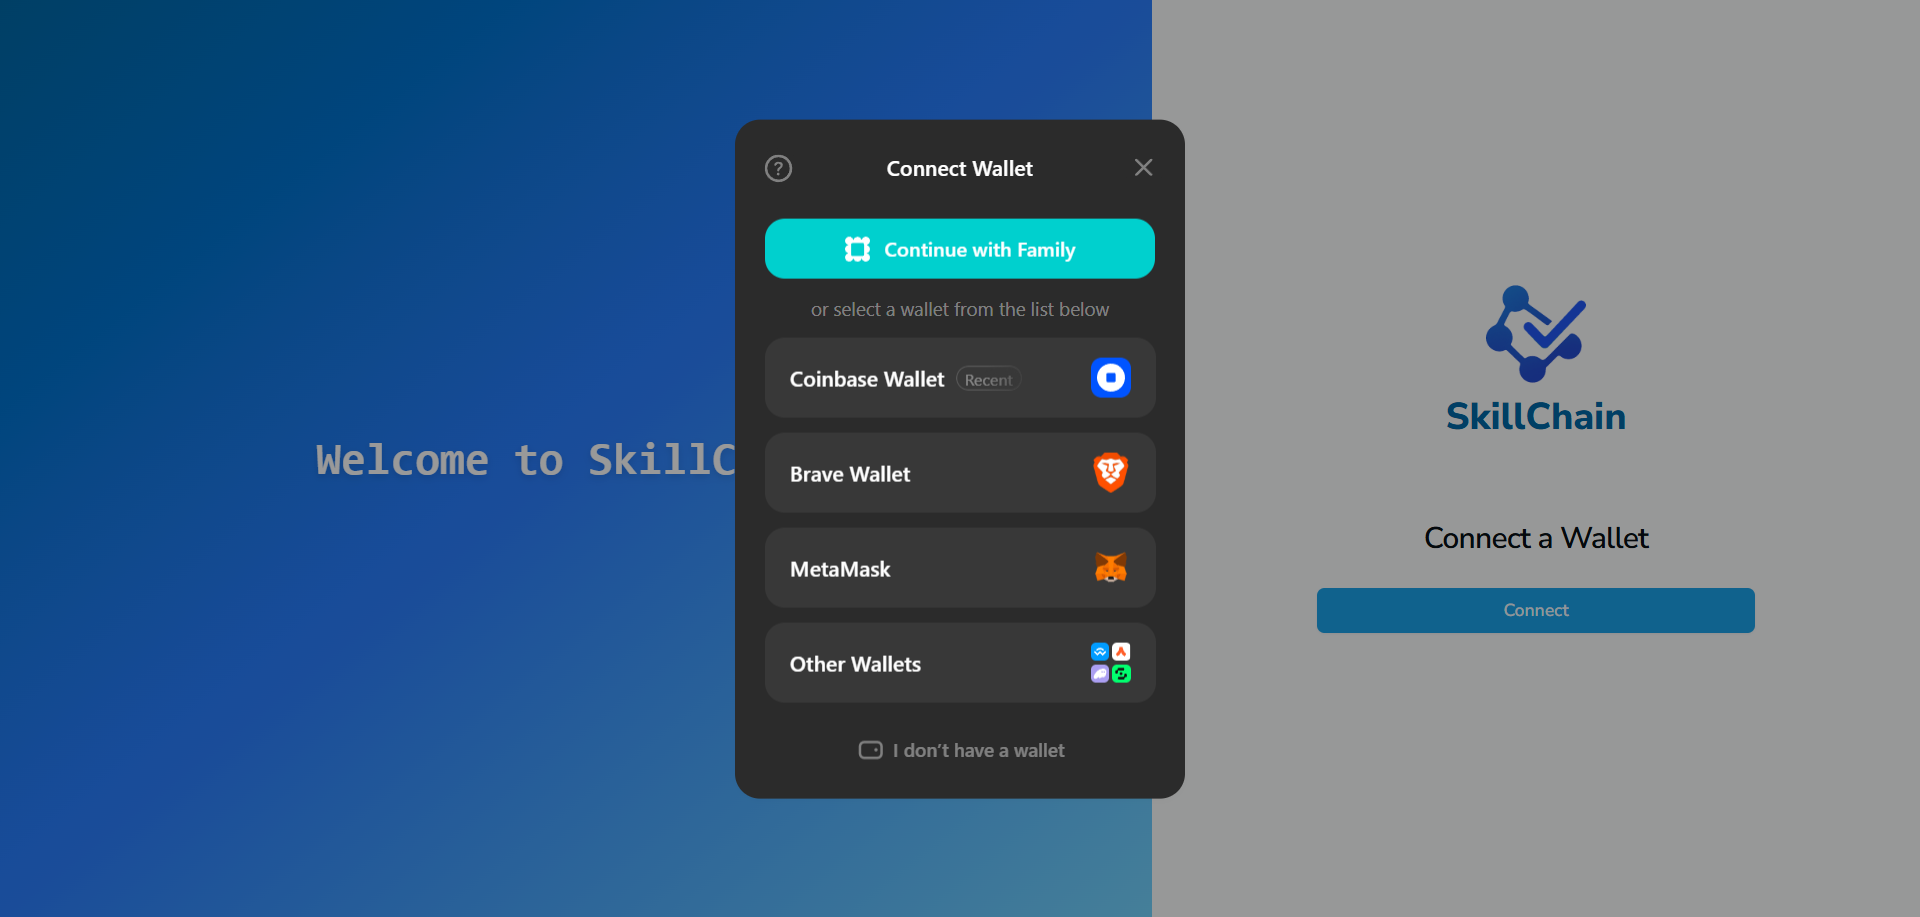
\includegraphics[width=0.99\textwidth, frame]{ui/login-wallets-page.png}
  \caption{Hộp thoại chọn ví kết nối}
  \label{fig:login-wallets-page}
\end{figure}

Sau khi kết nối thành công, hệ thống sẽ điều hướng người dùng đến trang chủ.

\begin{figure}[H]
  \centering
  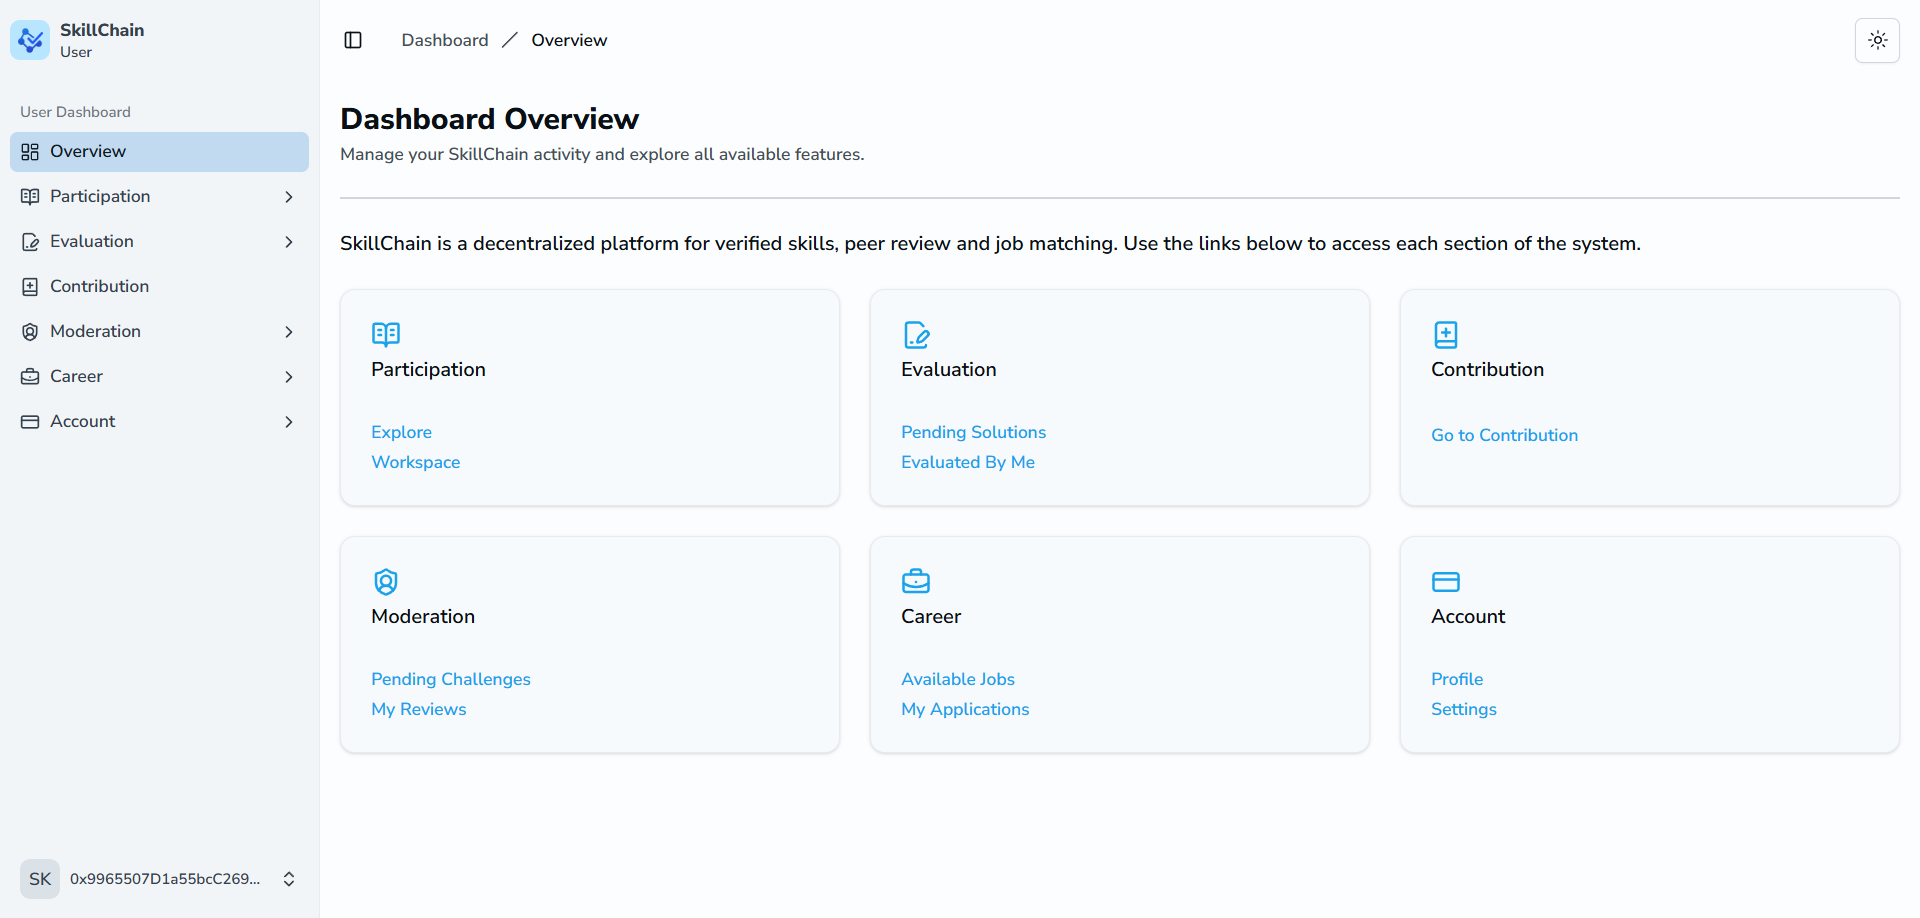
\includegraphics[width=0.99\textwidth, frame]{ui/home-page.png}
  \caption{Trang chủ}
  \label{fig:home-page}
\end{figure}

\subsection{Quản lý tài khoản}

\subsubsection{Thông tin cá nhân}

Để xem thông tin cá nhân, người dùng cần chọn \textbf{Account} $\rightarrow$ \textbf{Profile}.

\begin{figure}[H]
  \centering
  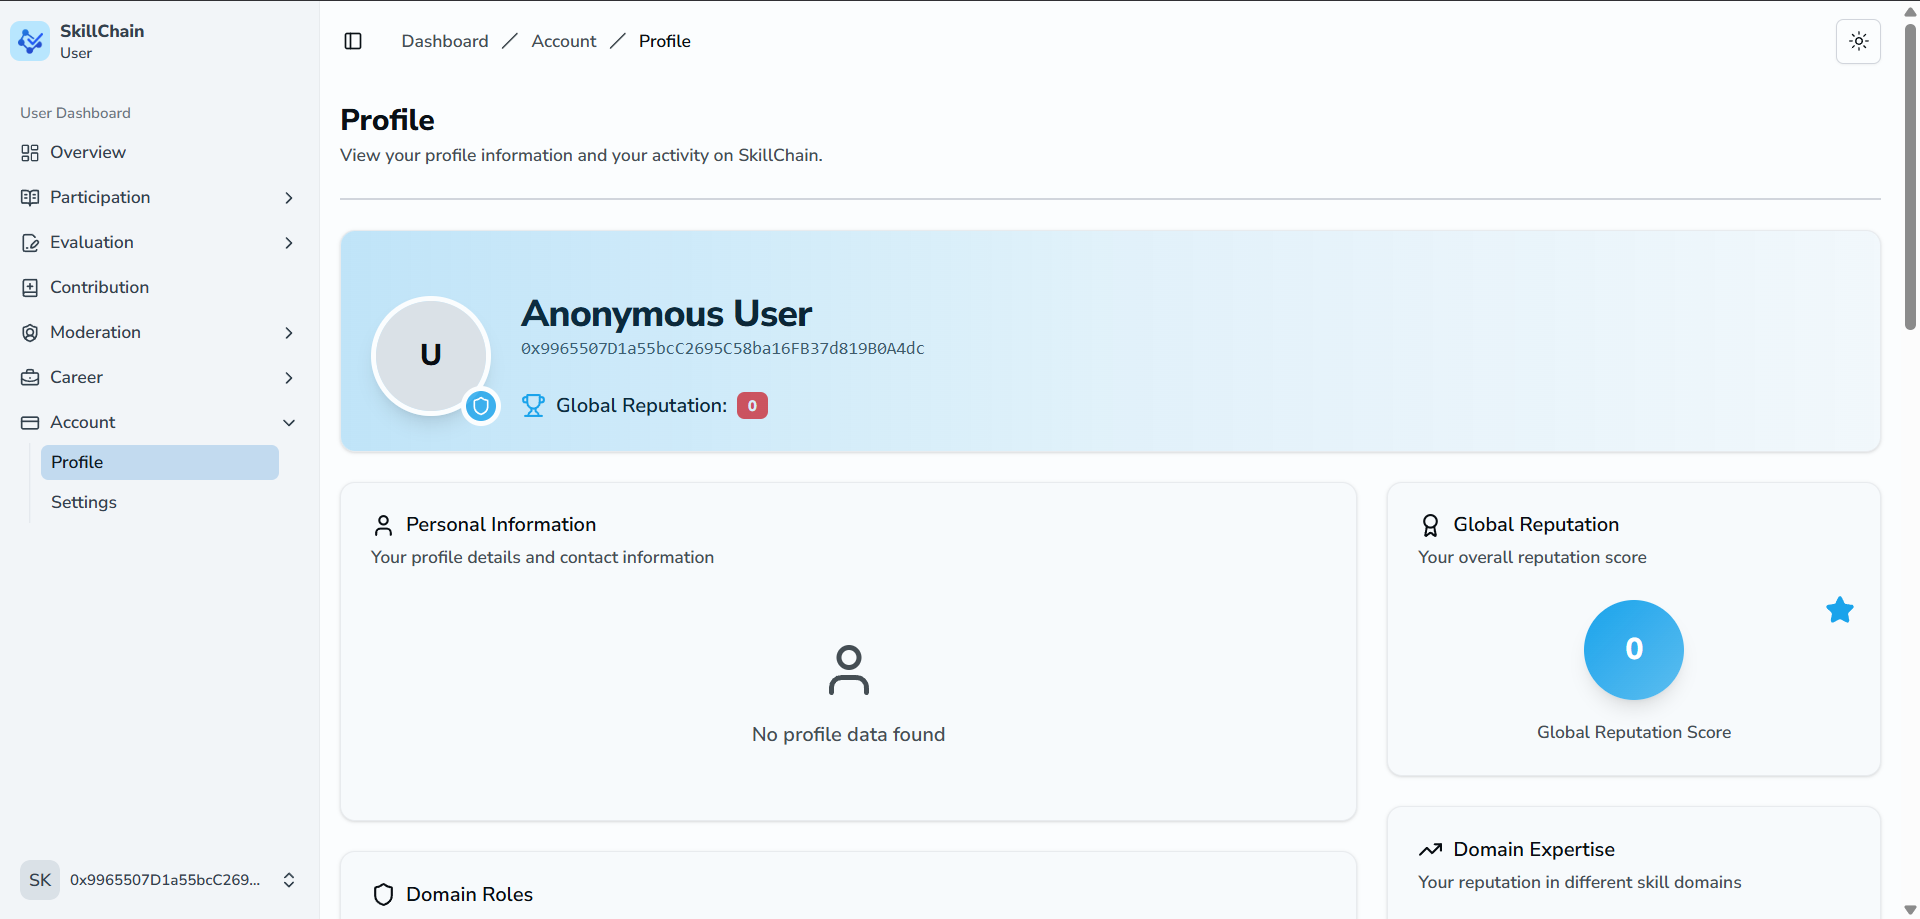
\includegraphics[width=0.99\textwidth, frame]{ui/unregistered-account-page.png}
  \caption{Trang thông tin tài khoản khi chưa đăng ký}
  \label{fig:unregistered-account-page}
\end{figure}

Ở góc dưới bên trái, hệ thống hiển thị quyền của người dùng đối với từng lĩnh vực chuyên môn, bao gồm khả năng đóng góp, kiểm duyệt và đánh giá.

\begin{figure}[H]
  \centering
  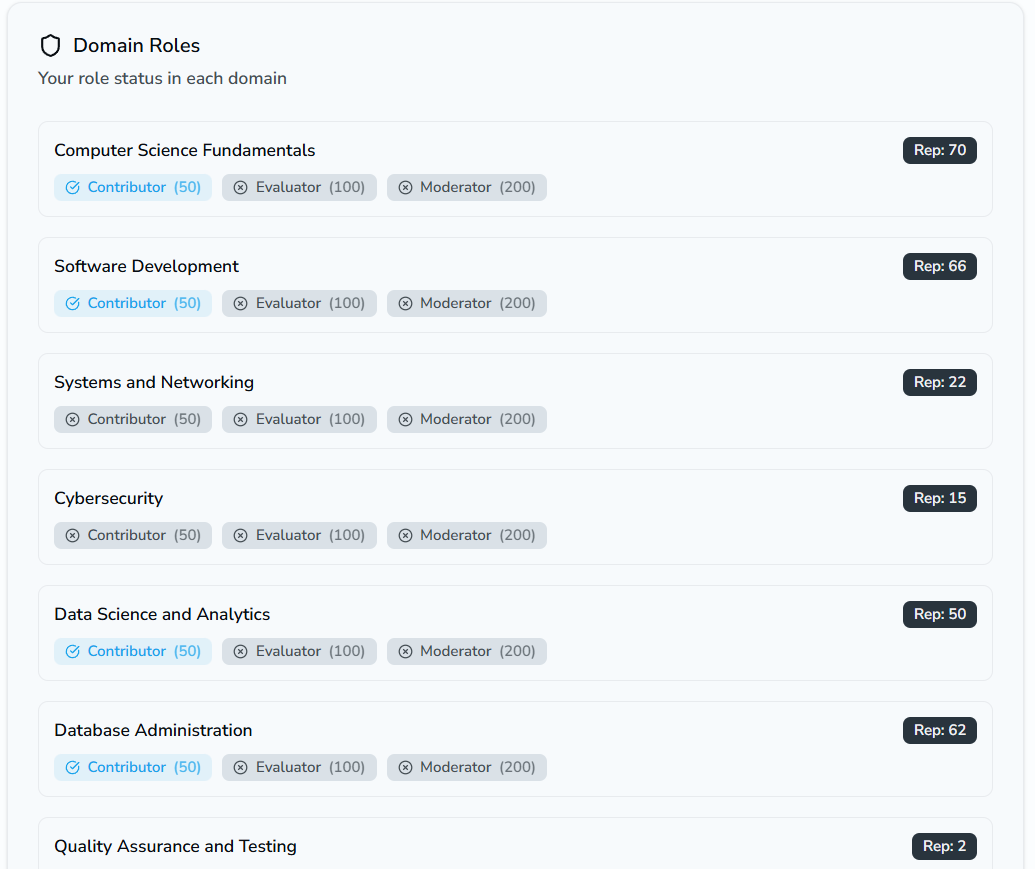
\includegraphics[width=0.99\textwidth, frame]{ui/domain-roles-page.png}
  \caption{Bảng vai trò của người dùng theo lĩnh vực chuyên môn}
  \label{fig:domain-roles-page}
\end{figure}

Hồ sơ uy tín được hiển thị ở góc dưới bên phải, bao gồm chỉ số uy tín toàn cục và uy tín theo từng lĩnh vực chuyên môn.

\begin{figure}[H]
  \centering
  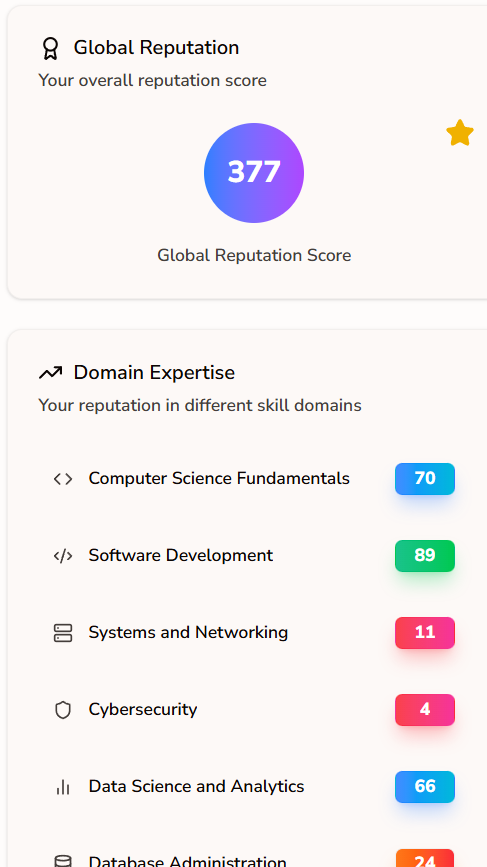
\includegraphics[width=0.5\textwidth, frame]{ui/reputation-profile.png}
  \caption{Hồ sơ uy tín}
  \label{fig:reputation-profile}
\end{figure}

\subsubsection{Cài đặt tài khoản}

Để chỉnh sửa thông tin cá nhân hoặc đăng ký tài khoản (nếu là lần kết nối đầu tiên), người dùng cần chọn \textbf{Account} $\rightarrow$ \textbf{Settings} và chuyển đến tab \textbf{Profile}.
Tại đây, người dùng có thể chọn ảnh đại diện, điền họ tên, địa chỉ email, nơi cư trú và tiểu sử để chỉnh sửa hoặc đăng ký thông tin cá nhân.  
Đối với lần đăng ký đầu tiên, hệ thống sẽ yêu cầu người dùng xác nhận giao dịch thông qua ví tiền điện tử để hoàn tất quá trình.

\begin{figure}[H]
  \centering
  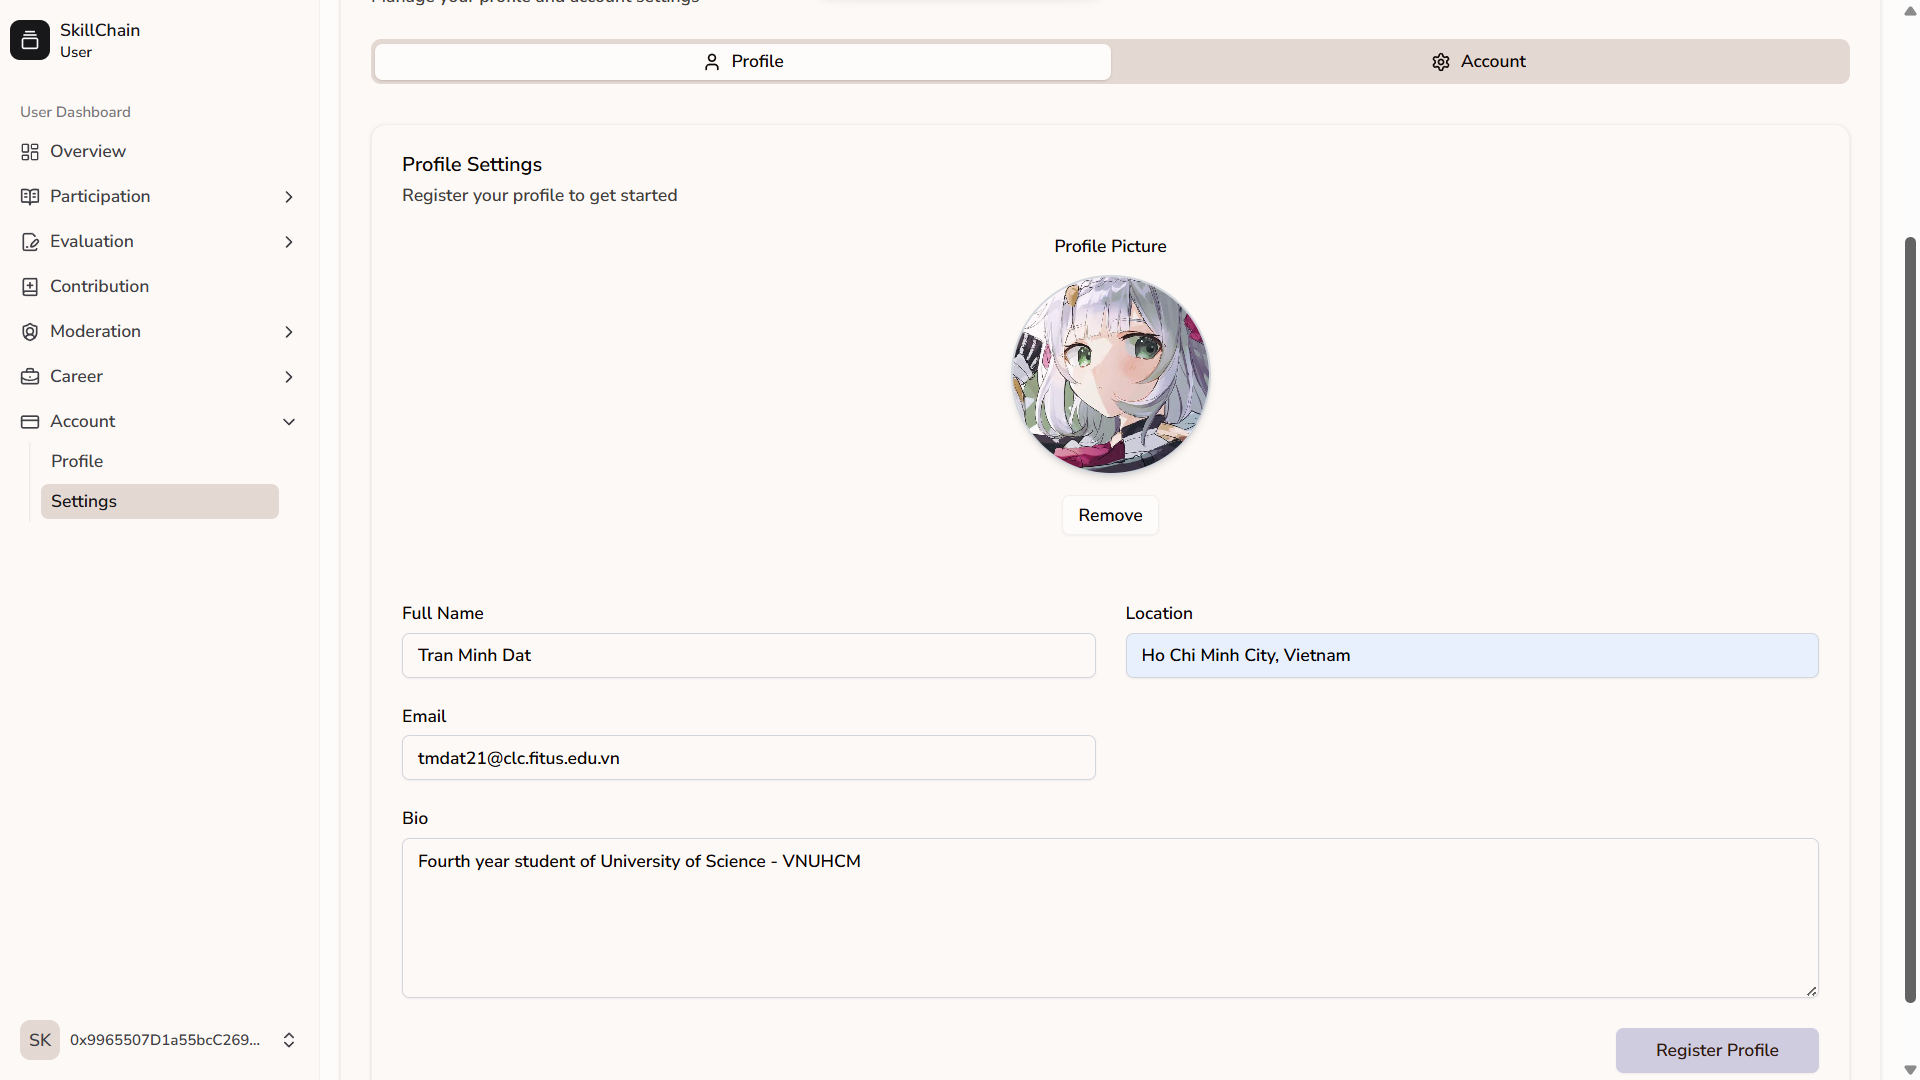
\includegraphics[width=0.99\textwidth, frame]{ui/register-account.png}
  \caption{Trang đăng ký thông tin cá nhân}
  \label{fig:register-account}
\end{figure}

\begin{figure}[H]
  \centering
  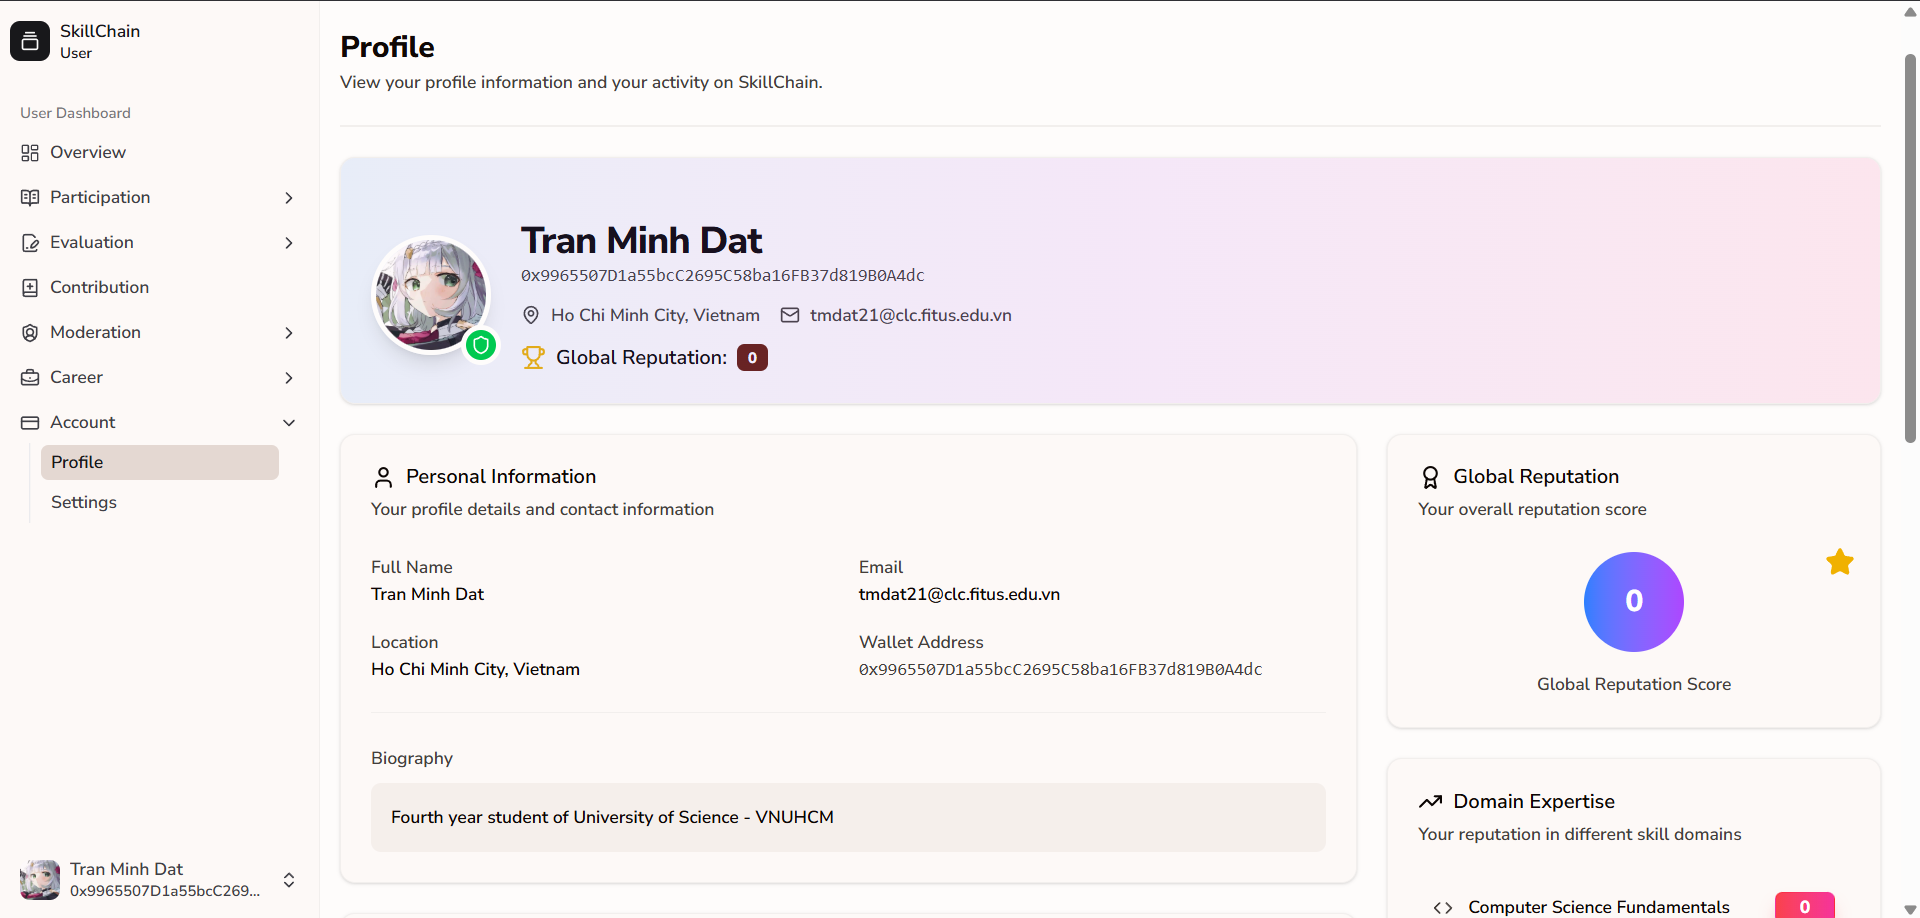
\includegraphics[width=0.99\textwidth, frame]{ui/registered-account-page.png}
  \caption{Trang thông tin cá nhân sau khi đã đăng ký}
  \label{fig:registered-account-page}
\end{figure}

Ngoài ra, người dùng cũng có thể truy cập tab \textbf{Account} để xem và cấu hình thông tin tài khoản liên quan đến hệ thống.

\begin{figure}[H]
  \centering
  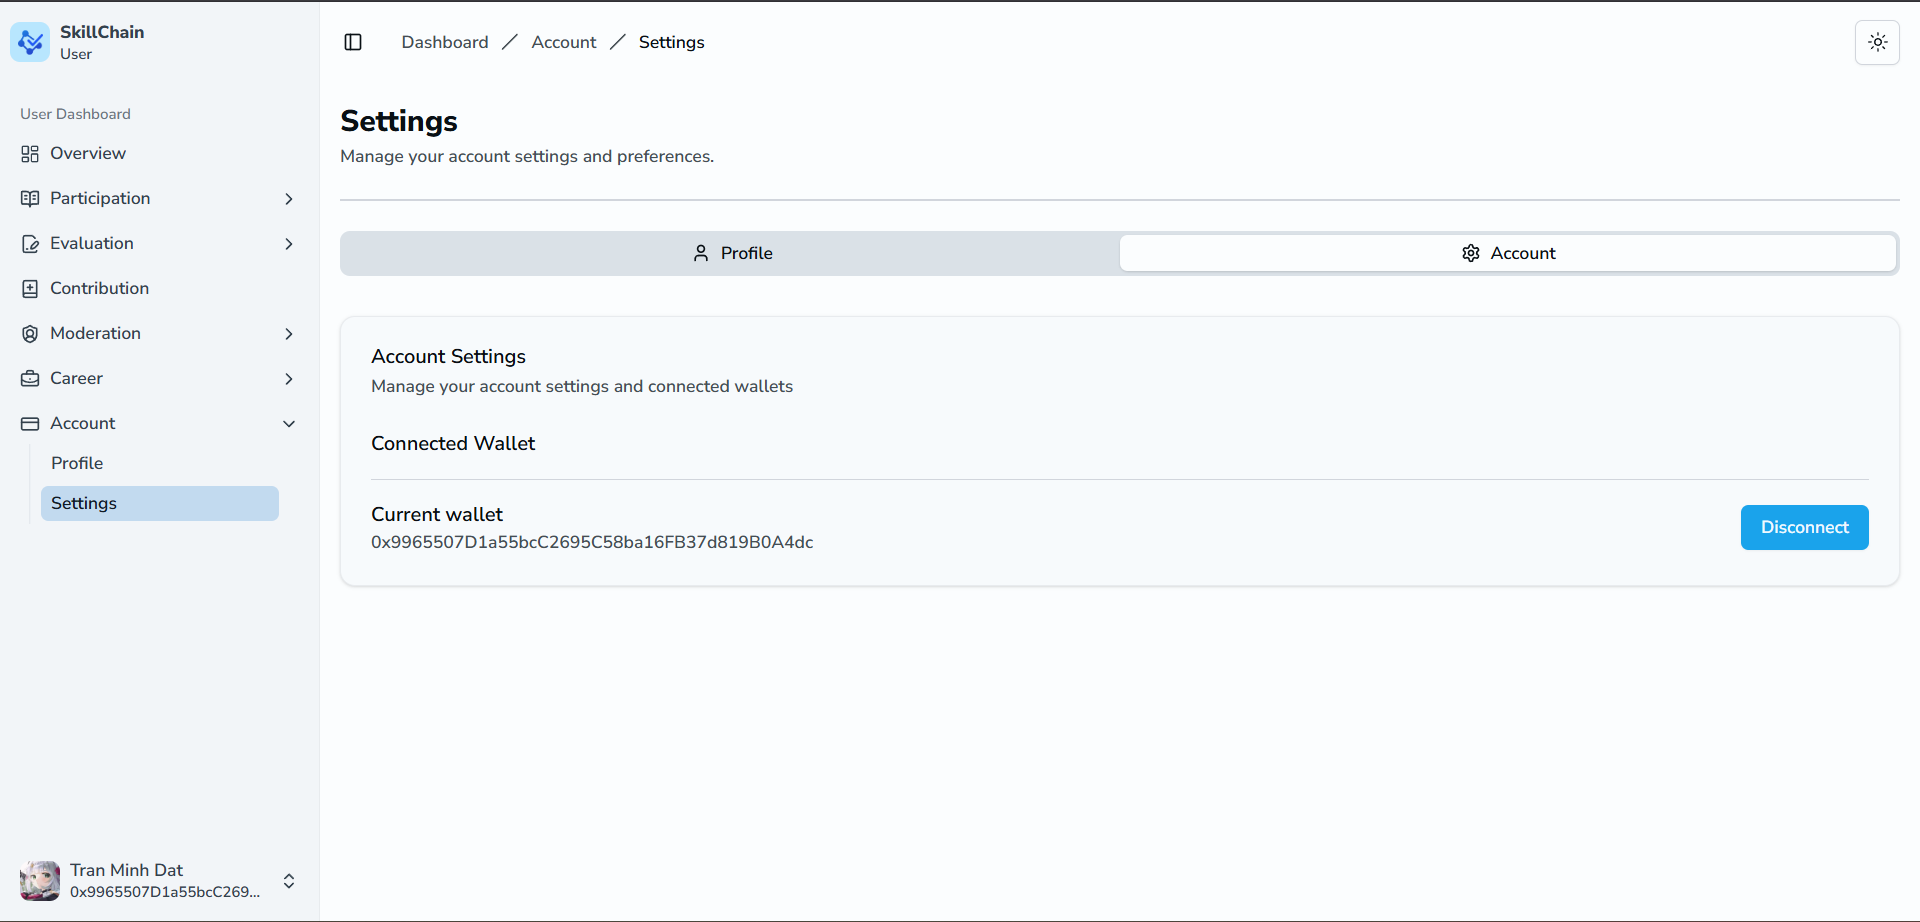
\includegraphics[width=0.99\textwidth, frame]{ui/account-settings-page.png}
  \caption{Trang thiết lập tài khoản}
  \label{fig:account-settings-page}
\end{figure}

\subsection{Đóng góp thử thách}

Để khởi tạo, quản lý và theo dõi các thử thách, người dùng cần truy cập tab \textbf{Contribution}.

\begin{figure}[H]
  \centering
  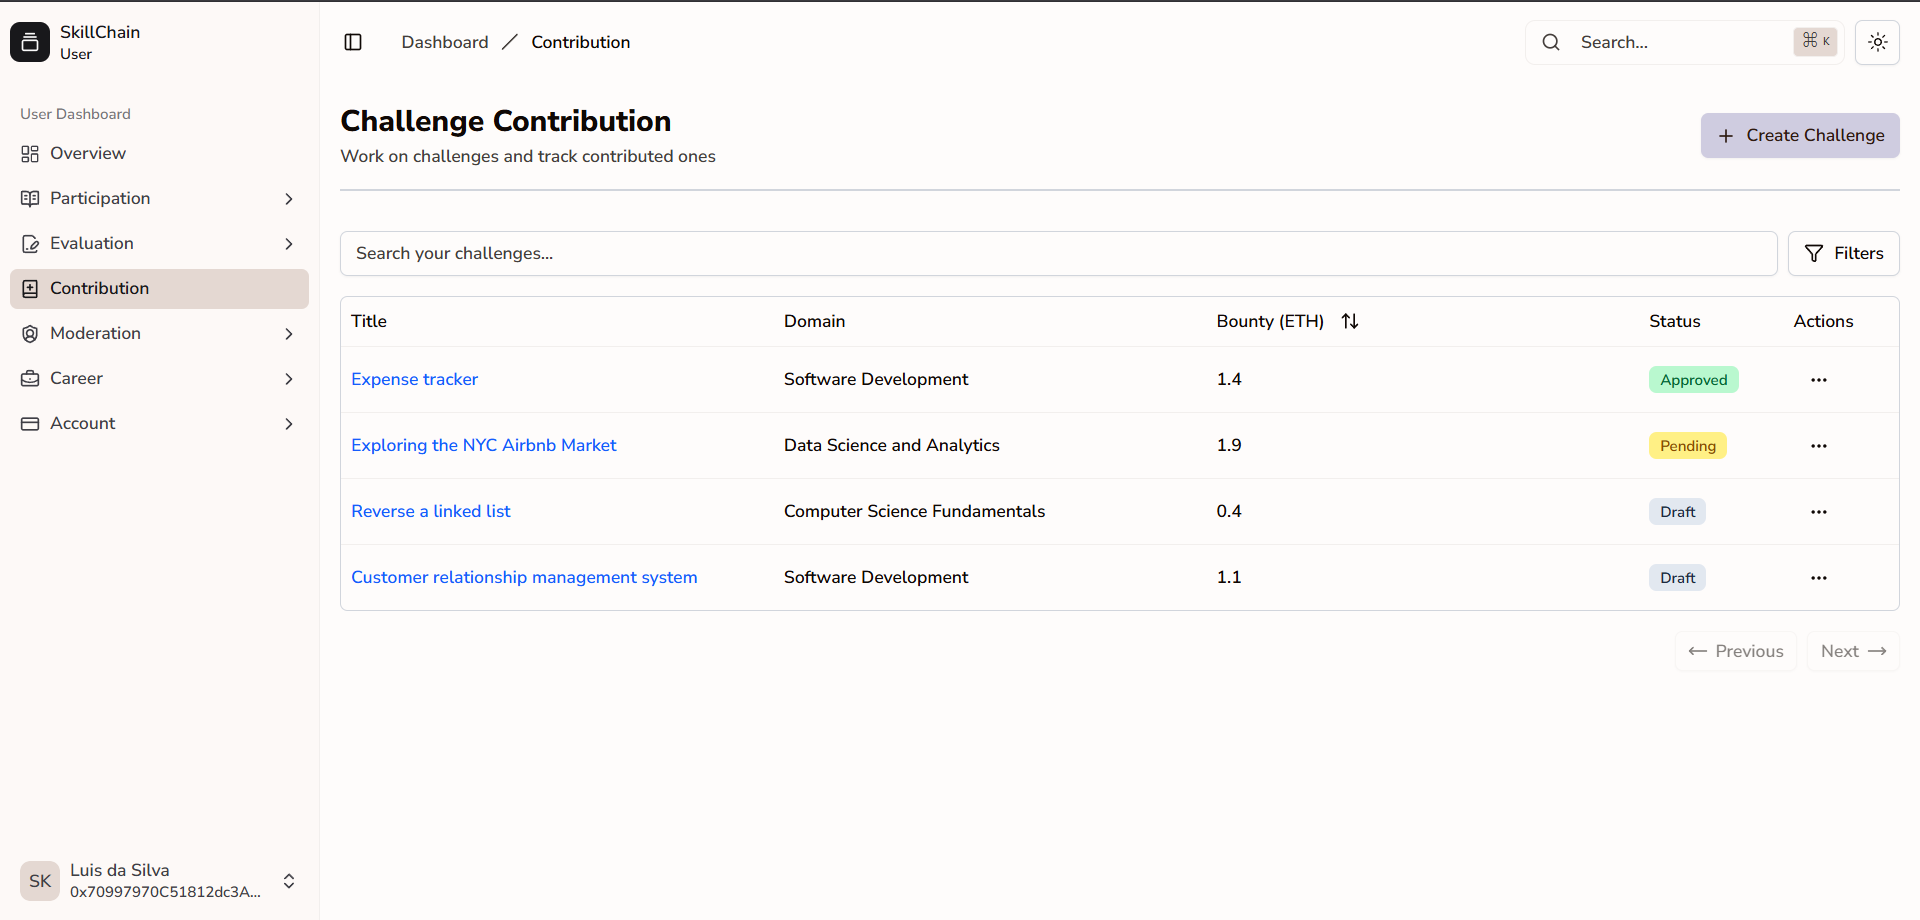
\includegraphics[width=0.99\textwidth, frame]{ui/contribution-page.png}
  \caption{Trang đóng góp thử thách}
  \label{fig:contribution-page}
\end{figure}

Tại đây, người dùng có thể xem danh sách các thử thách đã đóng góp, cùng với thông tin về loại thử thách, trạng thái và mức treo thưởng.  
Người dùng có thể xem chi tiết một thử thách bằng cách nhấn vào liên kết tên thử thách hoặc chọn ``View challenge'' từ nút ``Actions``.

\subsubsection{Tạo thử thách mới}

Để tạo một thử thách mới, người dùng nhấn nút ``Create Challenge'' ở góc trên bên phải.

\begin{figure}[H]
  \centering
  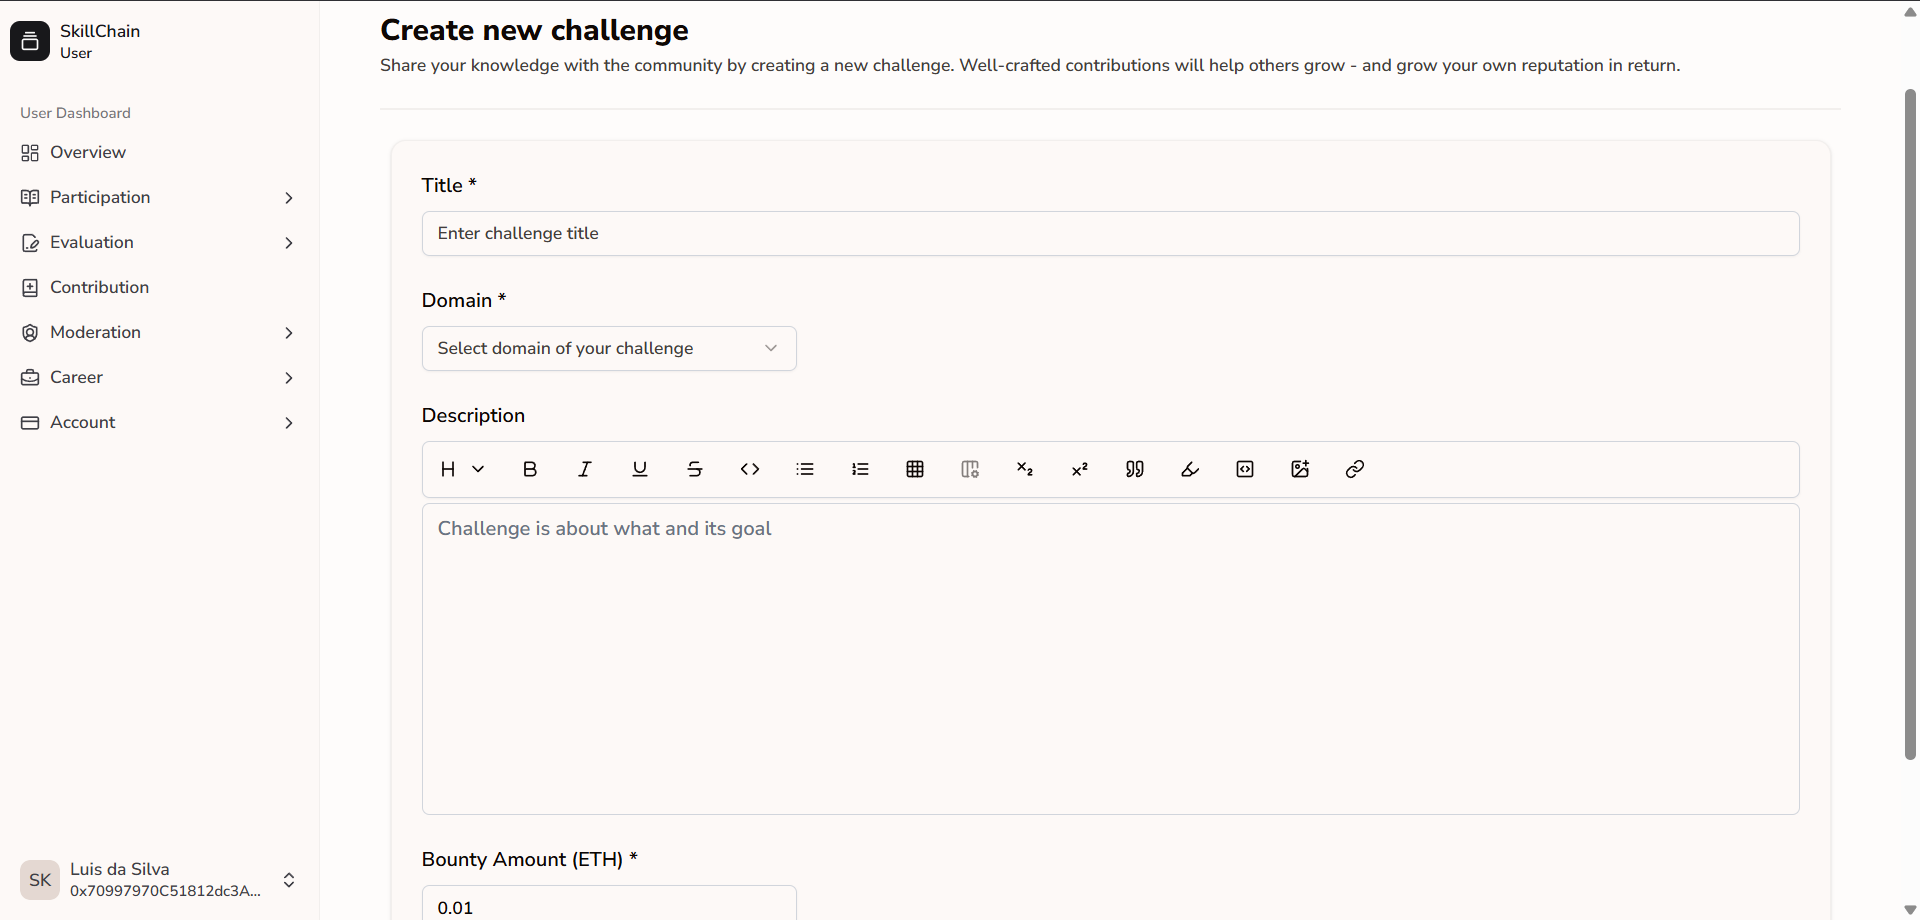
\includegraphics[width=0.99\textwidth, frame]{ui/create-challenge-page.png}
  \caption{Trang tạo thử thách mới}
  \label{fig:create-challenge-page}
\end{figure}

Tại trang này, người dùng nhập các thông tin quan trọng của thử thách, sau đó nhấn nút ``Create challenge''.  
Hệ thống sẽ yêu cầu xác thực giao dịch thông qua ví tiền điện tử để chính thức tạo thử thách ở trạng thái nháp.
Nếu người dùng không đủ chỉ số uy tín chuyên môn tương ứng với loại thử thách đang tạo, hệ thống sẽ hiển thị thông báo lỗi và không cho phép tạo thử thách.

\subsubsection{Chỉnh sửa thử thách}

Để chỉnh sửa một thử thách đang ở trạng thái nháp, người dùng cần truy cập trang chi tiết của thử thách và nhấn nút ``Edit''.

\begin{figure}[H]
  \centering
  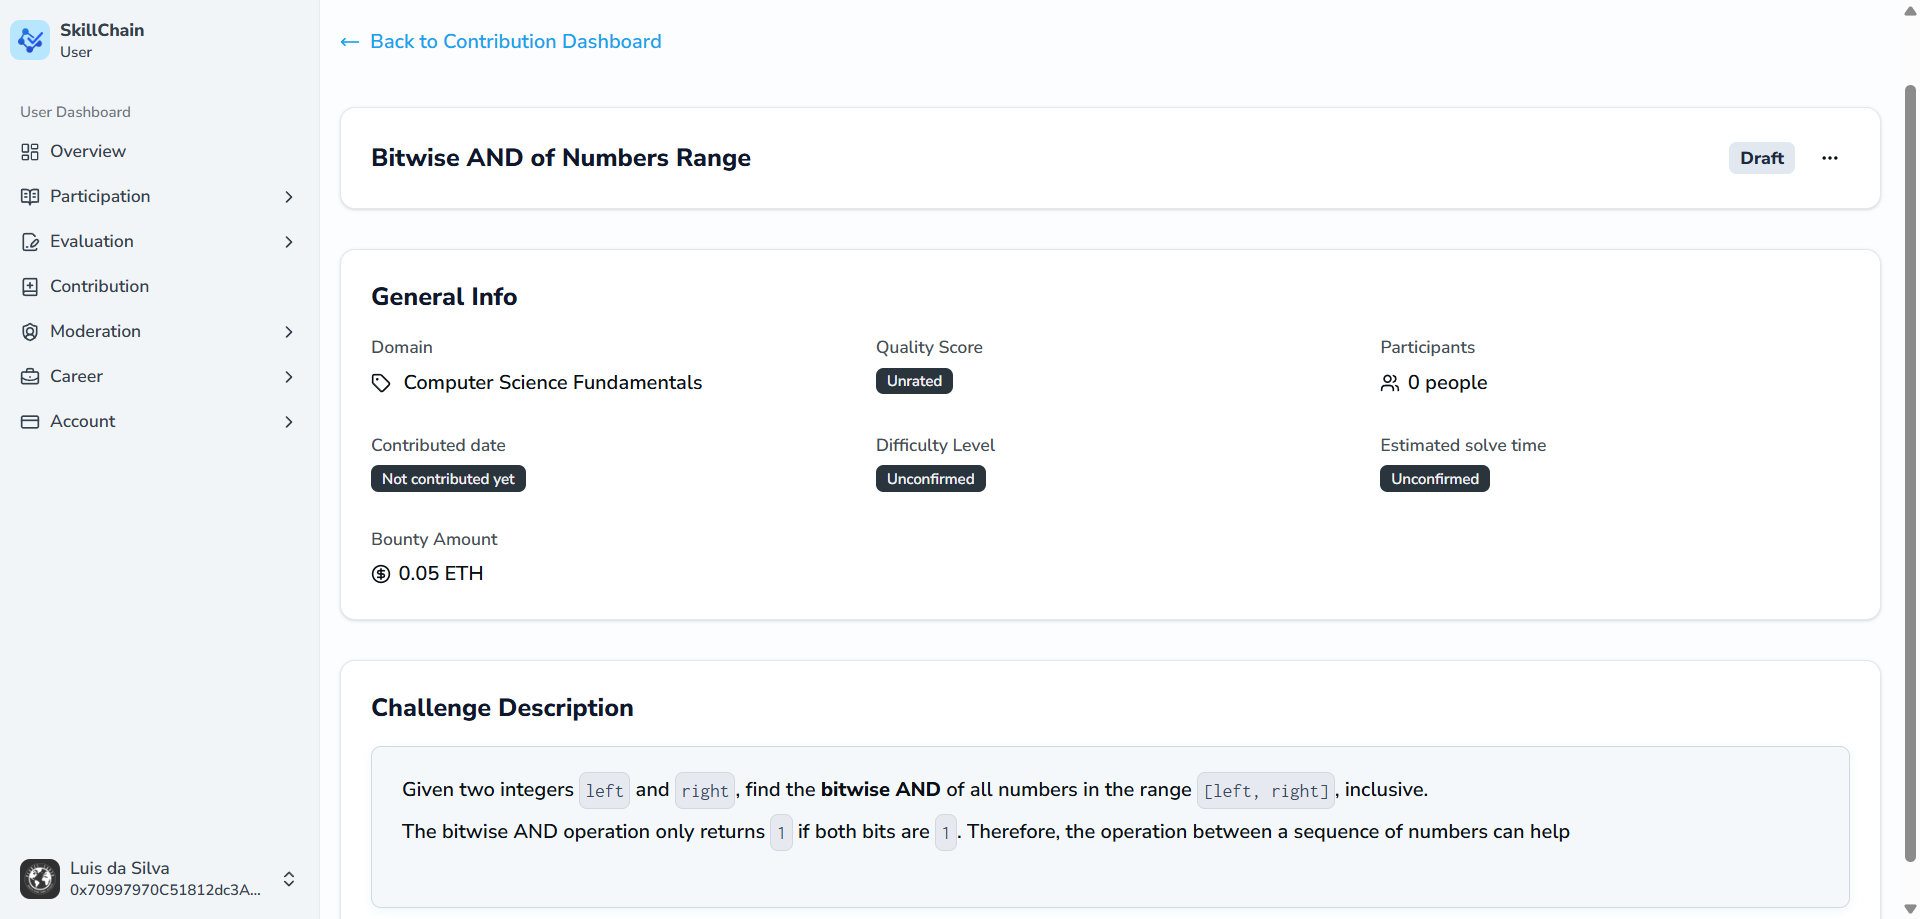
\includegraphics[width=0.99\textwidth, frame]{ui/contribution-challenge-detail-page.png}
  \caption{Trang chi tiết thử thách đã tạo}
  \label{fig:contribution-challenge-detail-page}
\end{figure}

\begin{figure}[H]
  \centering
  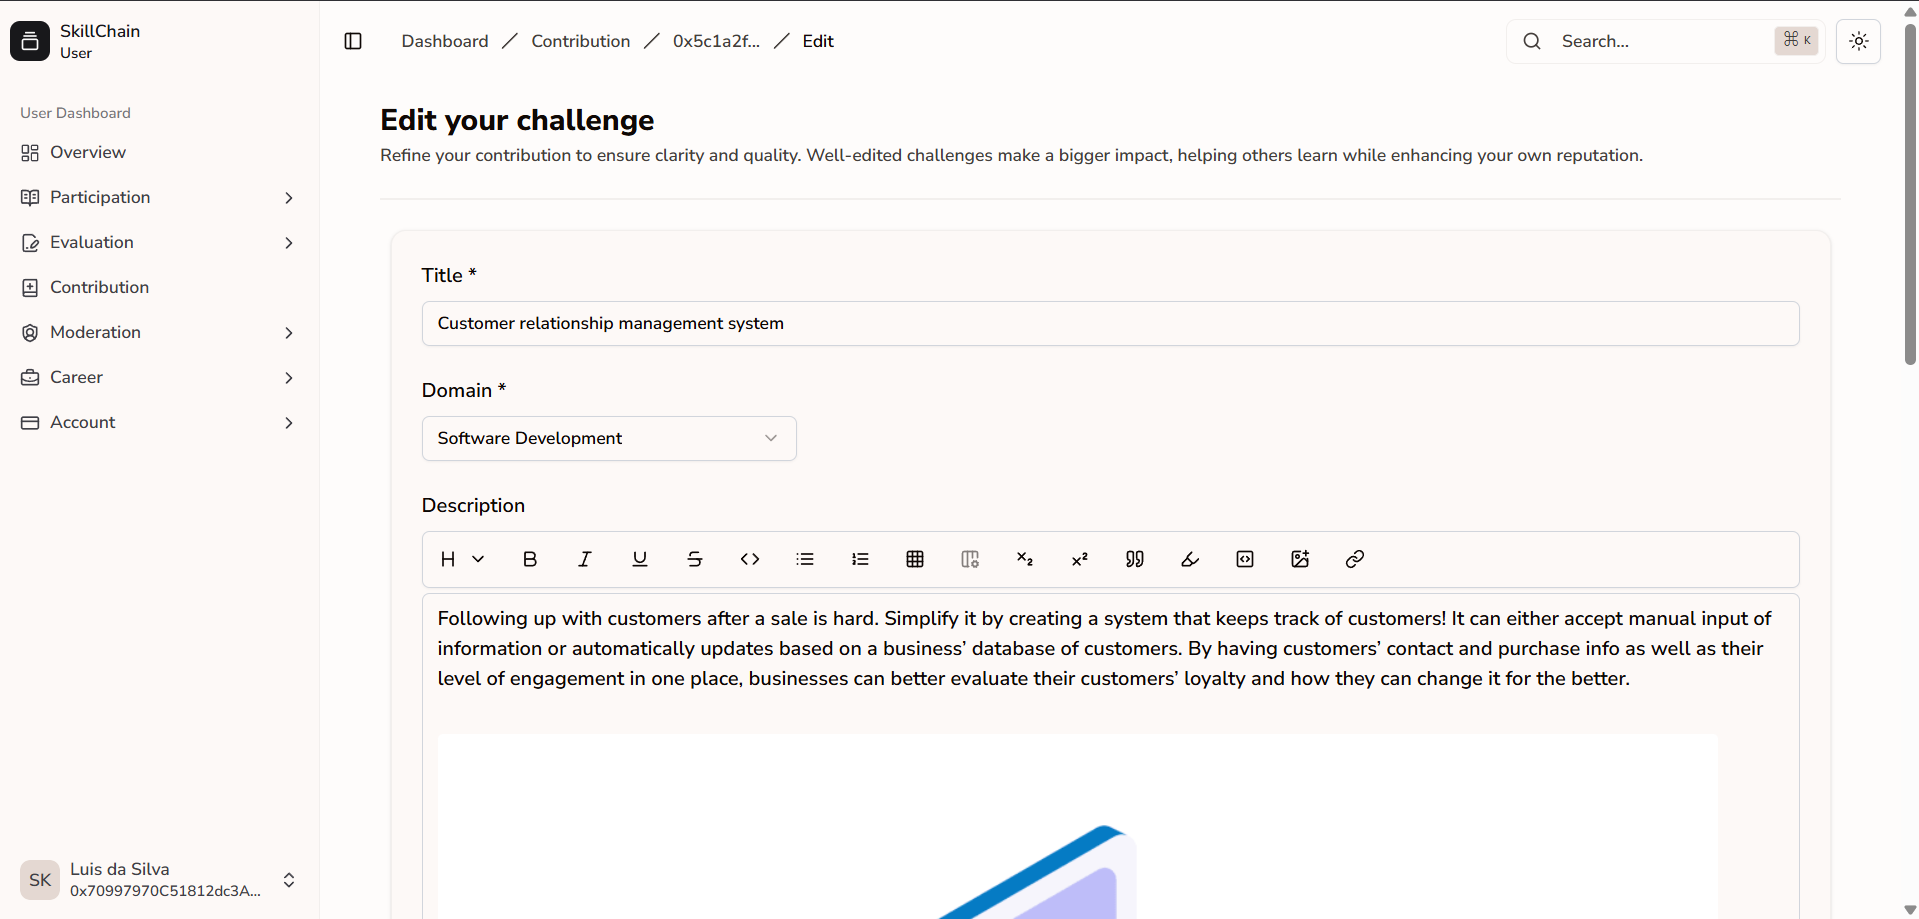
\includegraphics[width=0.99\textwidth, frame]{ui/contribution-challenge-edit-page.png}
  \caption{Trang chỉnh sửa thử thách}
  \label{fig:contribution-challenge-edit-page}
\end{figure}

Người dùng có thể chỉnh sửa nội dung thử thách tại đây và nhấn ``Save changes'' để lưu thay đổi.

\subsubsection{Gửi thử thách cho kiểm duyệt}

Để gửi thử thách đến bên kiểm duyệt, người dùng truy cập trang chi tiết của thử thách và nhấn nút ``Contribute''.  
Hệ thống sẽ yêu cầu xác thực giao dịch thông qua ví tiền điện tử để chính thức chuyển thử thách sang trạng thái chờ kiểm duyệt.  
Sau khi gửi đi, thử thách sẽ bị khóa và không còn có thể chỉnh sửa được nữa.

\subsection{Kiểm duyệt thử thách}

\subsubsection{Xem thử thách chờ kiểm duyệt}

Để xem danh sách các thử thách đang chờ kiểm duyệt, người dùng truy cập \textbf{Moderation} $\rightarrow$ \textbf{Pending Challenge}.  
Tại đây, người dùng có thể xem thông tin chi tiết từng thử thách, bao gồm số lượng người đã tham gia kiểm duyệt.

\begin{figure}[H]
  \centering
  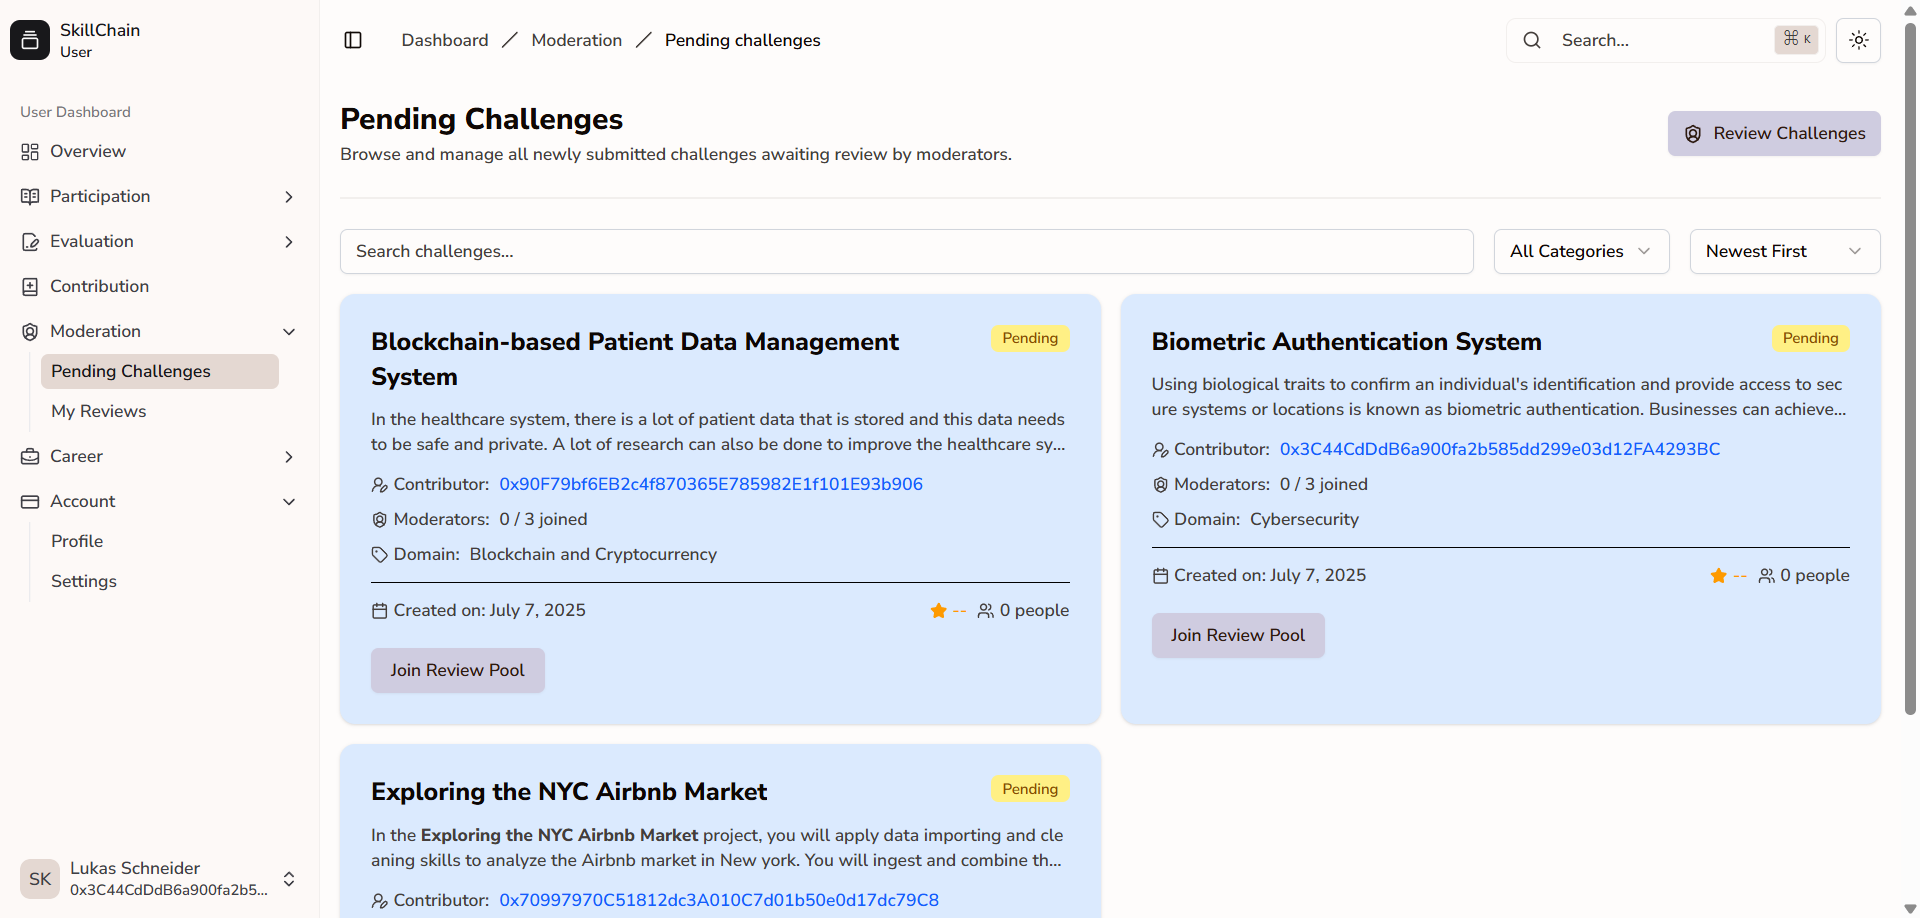
\includegraphics[width=0.99\textwidth, frame]{ui/moderation-pending-challenges-page.png}
  \caption{Trang danh sách thử thách chờ kiểm duyệt}
  \label{fig:moderation-pending-challenges-page}
\end{figure}

\subsubsection{Tham gia kiểm duyệt thử thách}

Để tham gia kiểm duyệt một thử thách, người dùng nhấn nút ``Join Review Pool'' tại thử thách mong muốn.  
Hệ thống sẽ yêu cầu xác thực giao dịch thông qua ví tiền điện tử để hoàn tất việc tham gia kiểm duyệt.
Nếu người dùng không đủ chỉ số uy tín chuyên môn tương ứng với loại thử thách, hệ thống sẽ hiển thị thông báo lỗi và không cho phép tham gia.

\subsubsection{Thực hiện kiểm duyệt}

Để bắt đầu kiểm duyệt, người dùng truy cập \textbf{Moderation} $\rightarrow$ \textbf{My Reviews} để xem danh sách các thử thách mà mình đã tham gia kiểm duyệt.  
Sau đó, chọn thử thách tương ứng và nhấn nút ``Edit review''.

\begin{figure}[H]
  \centering
  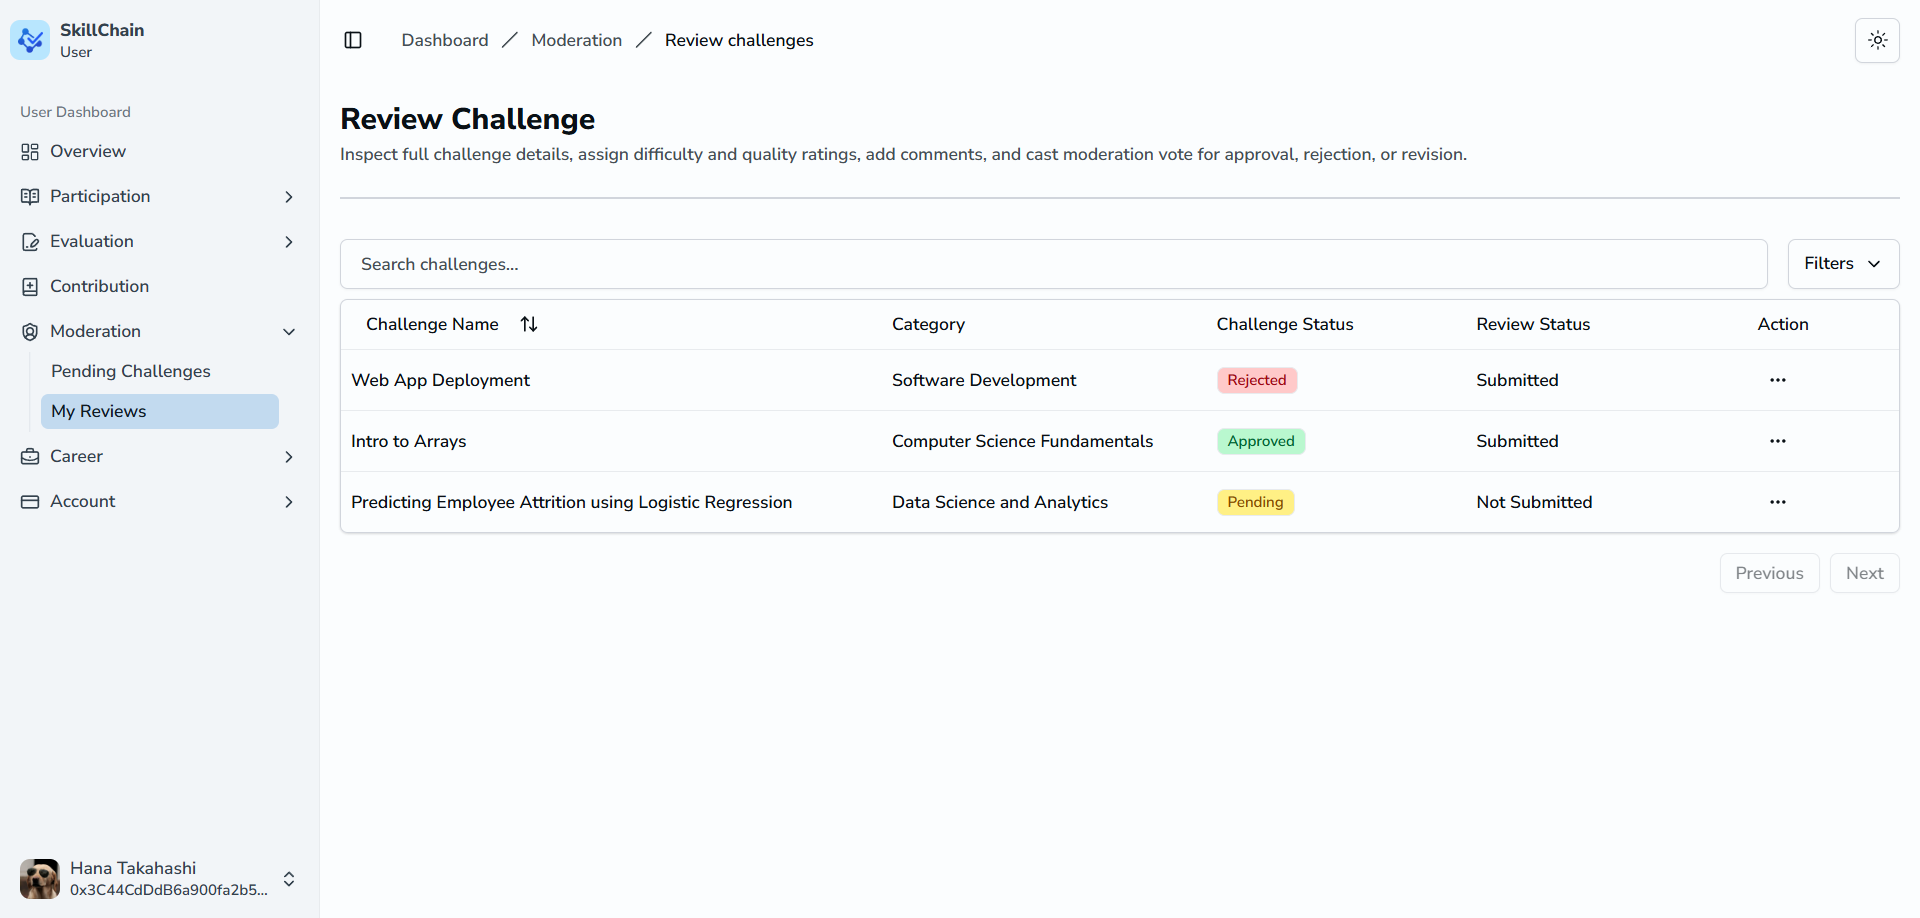
\includegraphics[width=0.99\textwidth, frame]{ui/moderation-my-reviews-page.png}
  \caption{Trang danh sách thử thách đã và đang kiểm duyệt}
  \label{fig:moderation-my-reviews-page}
\end{figure}

Tại trang này, người dùng có thể xem chi tiết phiên kiểm duyệt.  
Để thực hiện đánh giá, chuyển sang tab \textbf{Review Form}.

Trong biểu mẫu kiểm duyệt, người dùng cần:
\begin{itemize}
  \item Chọn \textbf{Yes/No} cho từng tiêu chí đánh giá chất lượng.
  \item Đề xuất độ khó và thời gian giải ước tính.
  \item Có thể lưu tạm nội dung đánh giá hoặc gửi luôn.
\end{itemize}

Sau khi hoàn tất, nhấn nút ``Submit Review'' để nộp đánh giá.  
Giao dịch sẽ cần được xác thực qua ví tiền điện tử, và sau khi gửi, nội dung đánh giá sẽ không thể chỉnh sửa.

\begin{figure}[H]
  \centering
  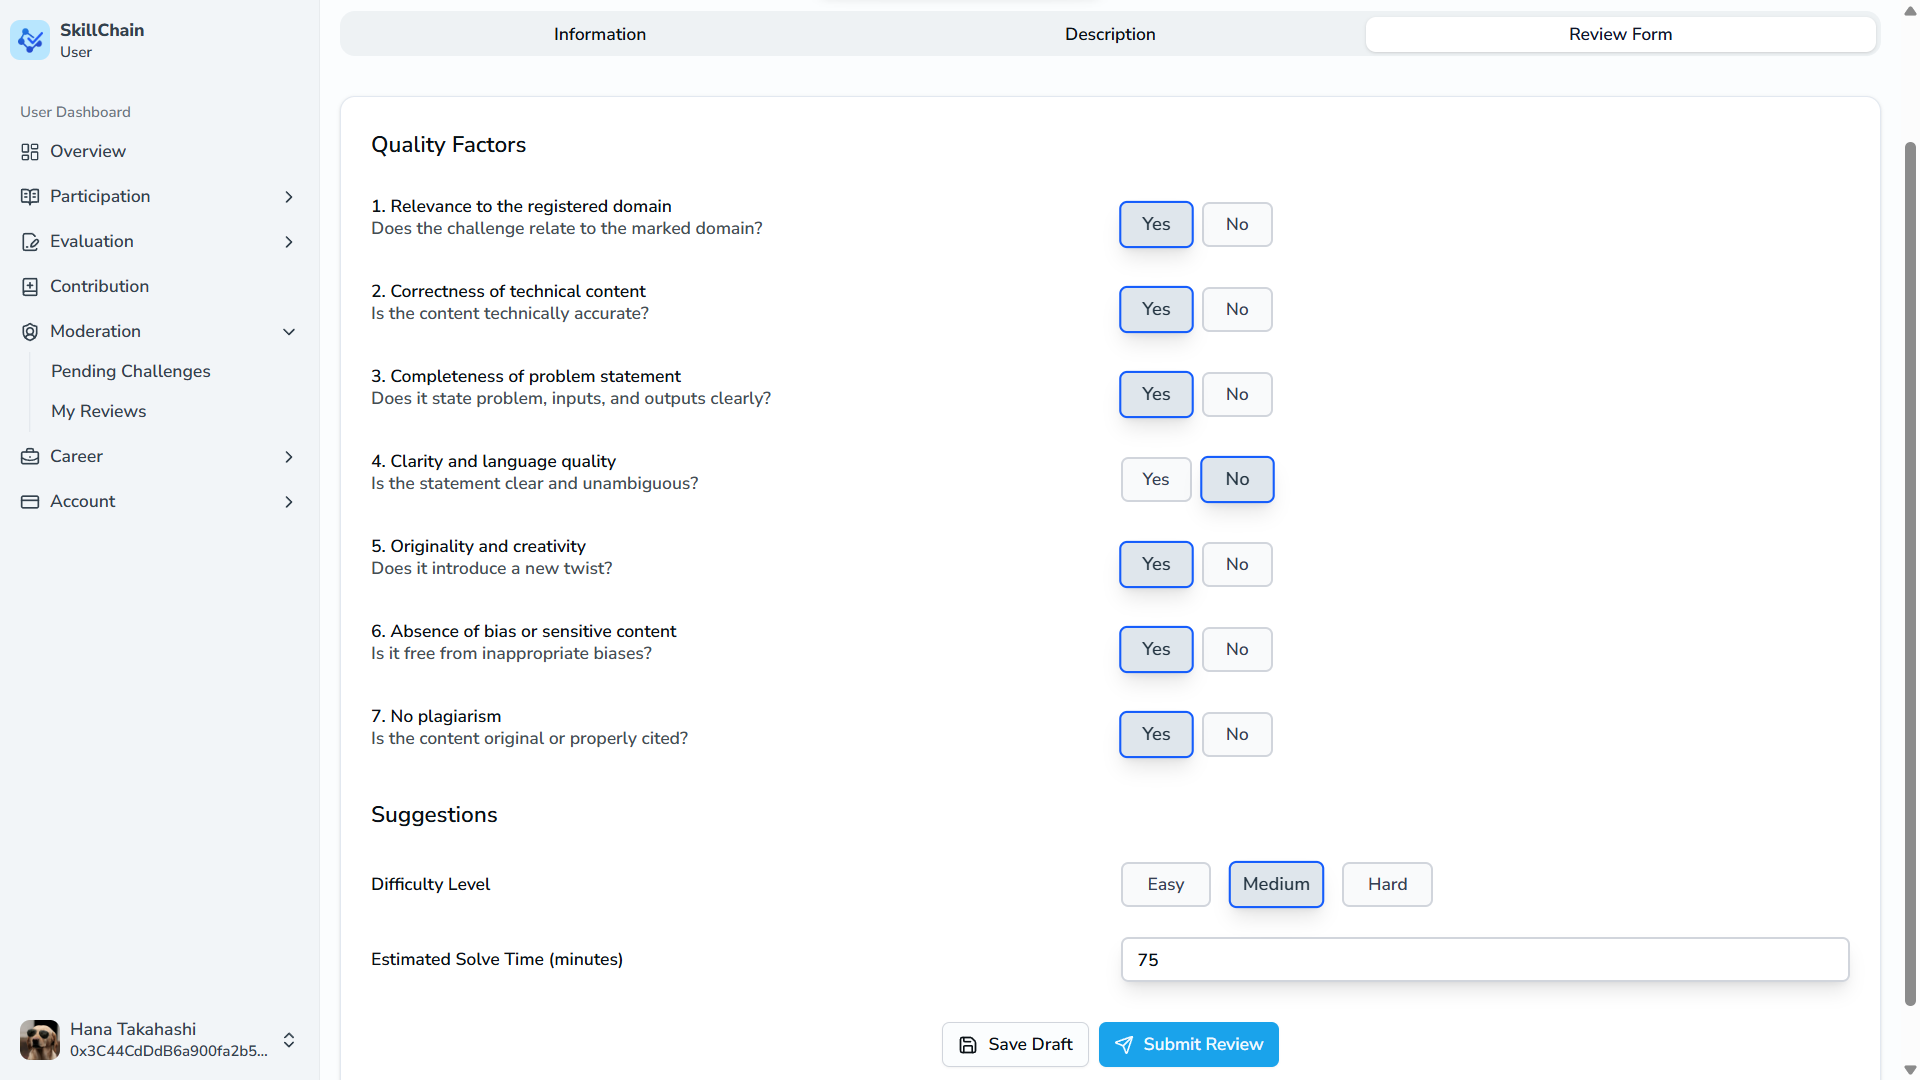
\includegraphics[width=0.99\textwidth, frame]{ui/moderation-review-form.png}
  \caption{Biểu mẫu kiểm duyệt chất lượng thử thách}
  \label{fig:moderation-review-form}
\end{figure}

\subsubsection{Xem thông tin phiên kiểm duyệt}

Khi phiên kiểm duyệt kết thúc, thông tin chi tiết về phiên sẽ được hiển thị cho người đóng góp và các kiểm duyệt viên.  
Thông tin này bao gồm danh sách người kiểm duyệt, số điểm đánh giá, và phần token thưởng tương ứng.

\begin{figure}[H]
  \centering
  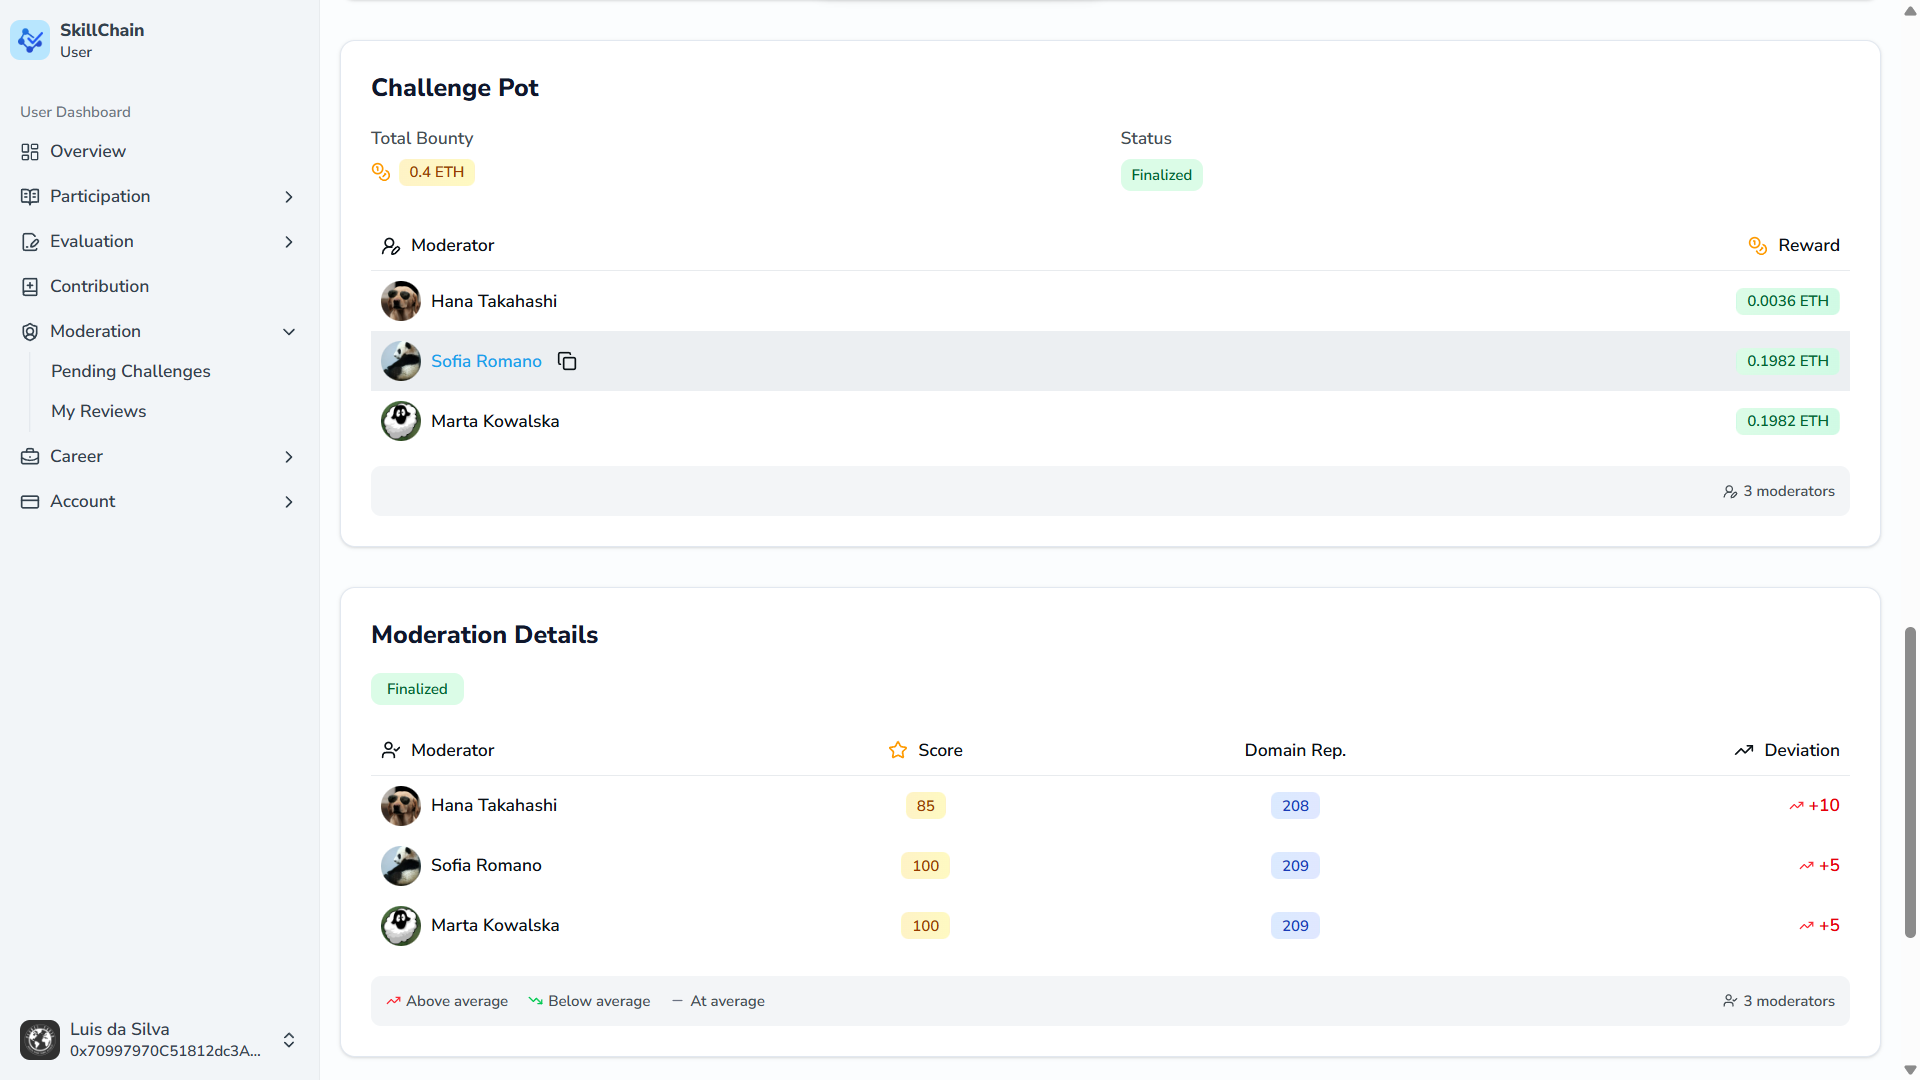
\includegraphics[width=0.99\textwidth, frame]{ui/challenge-moderation-pot-info.png}
  \caption{Thông tin chi tiết của một phiên kiểm duyệt}
  \label{fig:challenge-moderation-pot-info}
\end{figure}

\subsection{Tham gia thử thách}

\subsubsection{Xem thử thách đang hiện hành}

Để xem danh sách các thử thách đang mở, người dùng truy cập \textbf{Participation} $\rightarrow$ \textbf{Explore}.  
Tại đây, người dùng có thể xem chi tiết nội dung từng thử thách bằng cách nhấn vào thẻ tương ứng.

\begin{figure}[H]
  \centering
  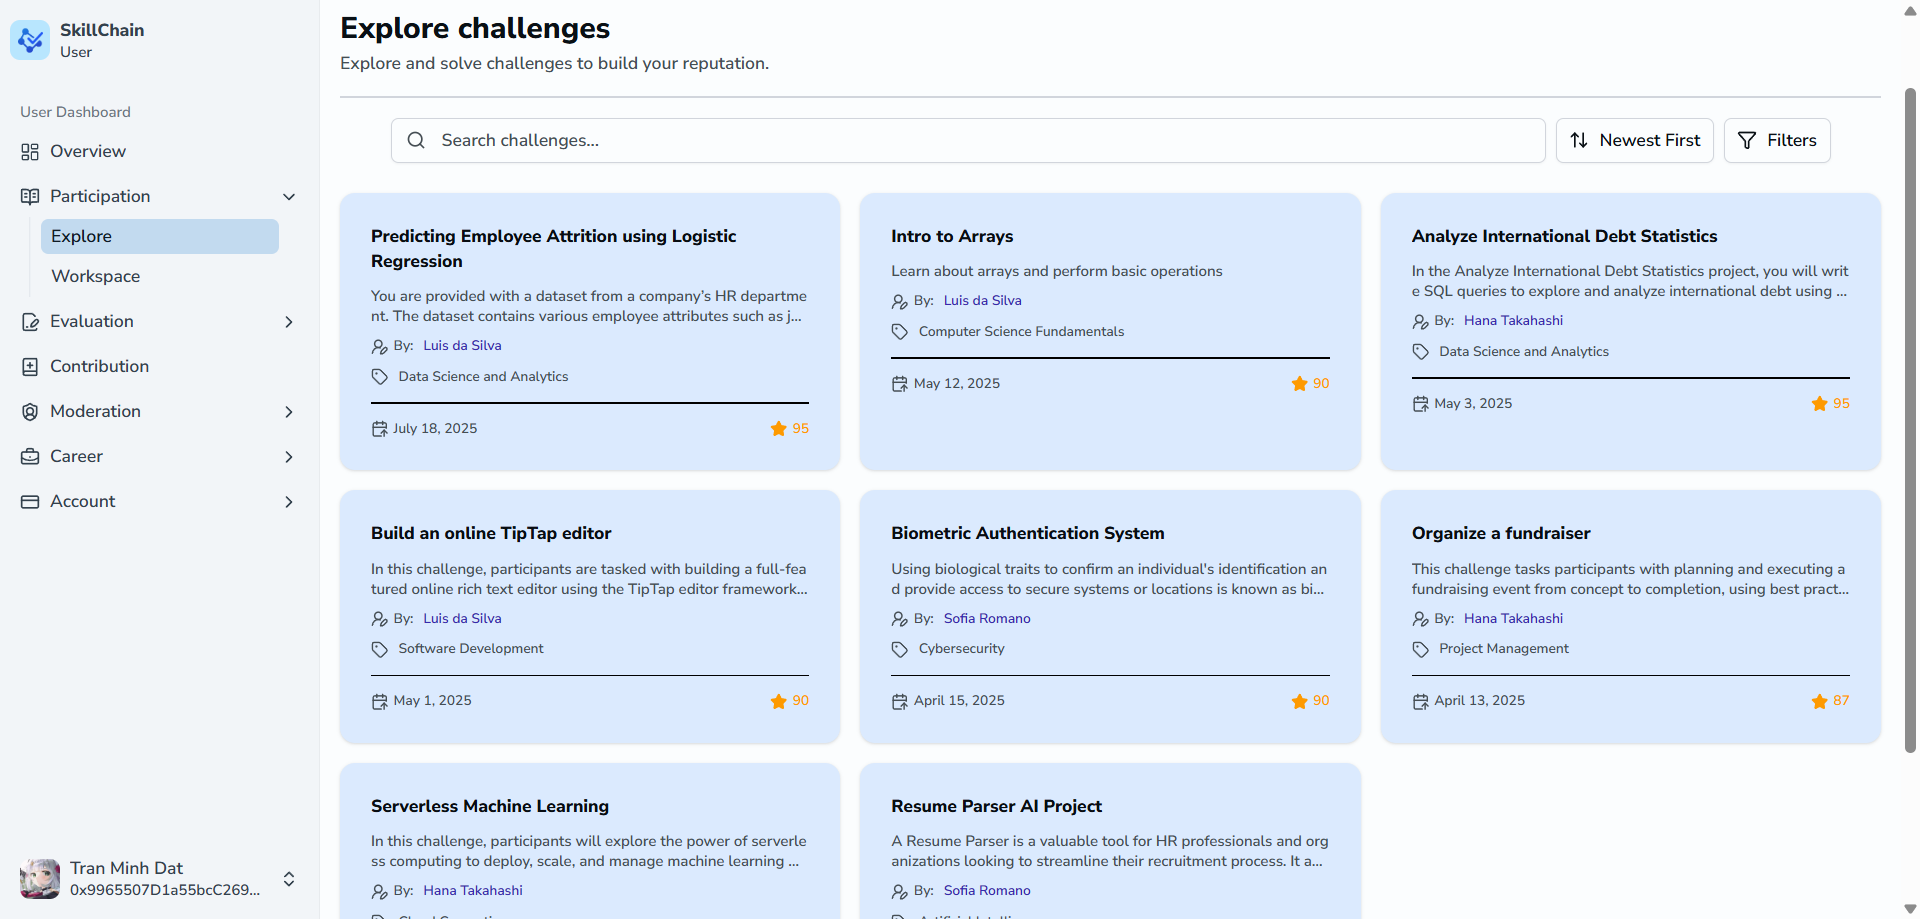
\includegraphics[width=0.99\textwidth, frame]{ui/explore-challenges-page.png}
  \caption{Trang danh sách thử thách đang hiện hành}
  \label{fig:explore-challenges-page}
\end{figure}

\subsubsection{Thực hiện thử thách}

Khi xem chi tiết nội dung một thử thách, người dùng có thể nhấn nút ``Join Challenge'' (ở góc trên hoặc góc dưới bên phải) để tham gia.  
Hệ thống sẽ yêu cầu người dùng xác nhận trả một khoản phí và xác thực giao dịch qua ví tiền điện tử.

\begin{figure}[H]
  \centering
  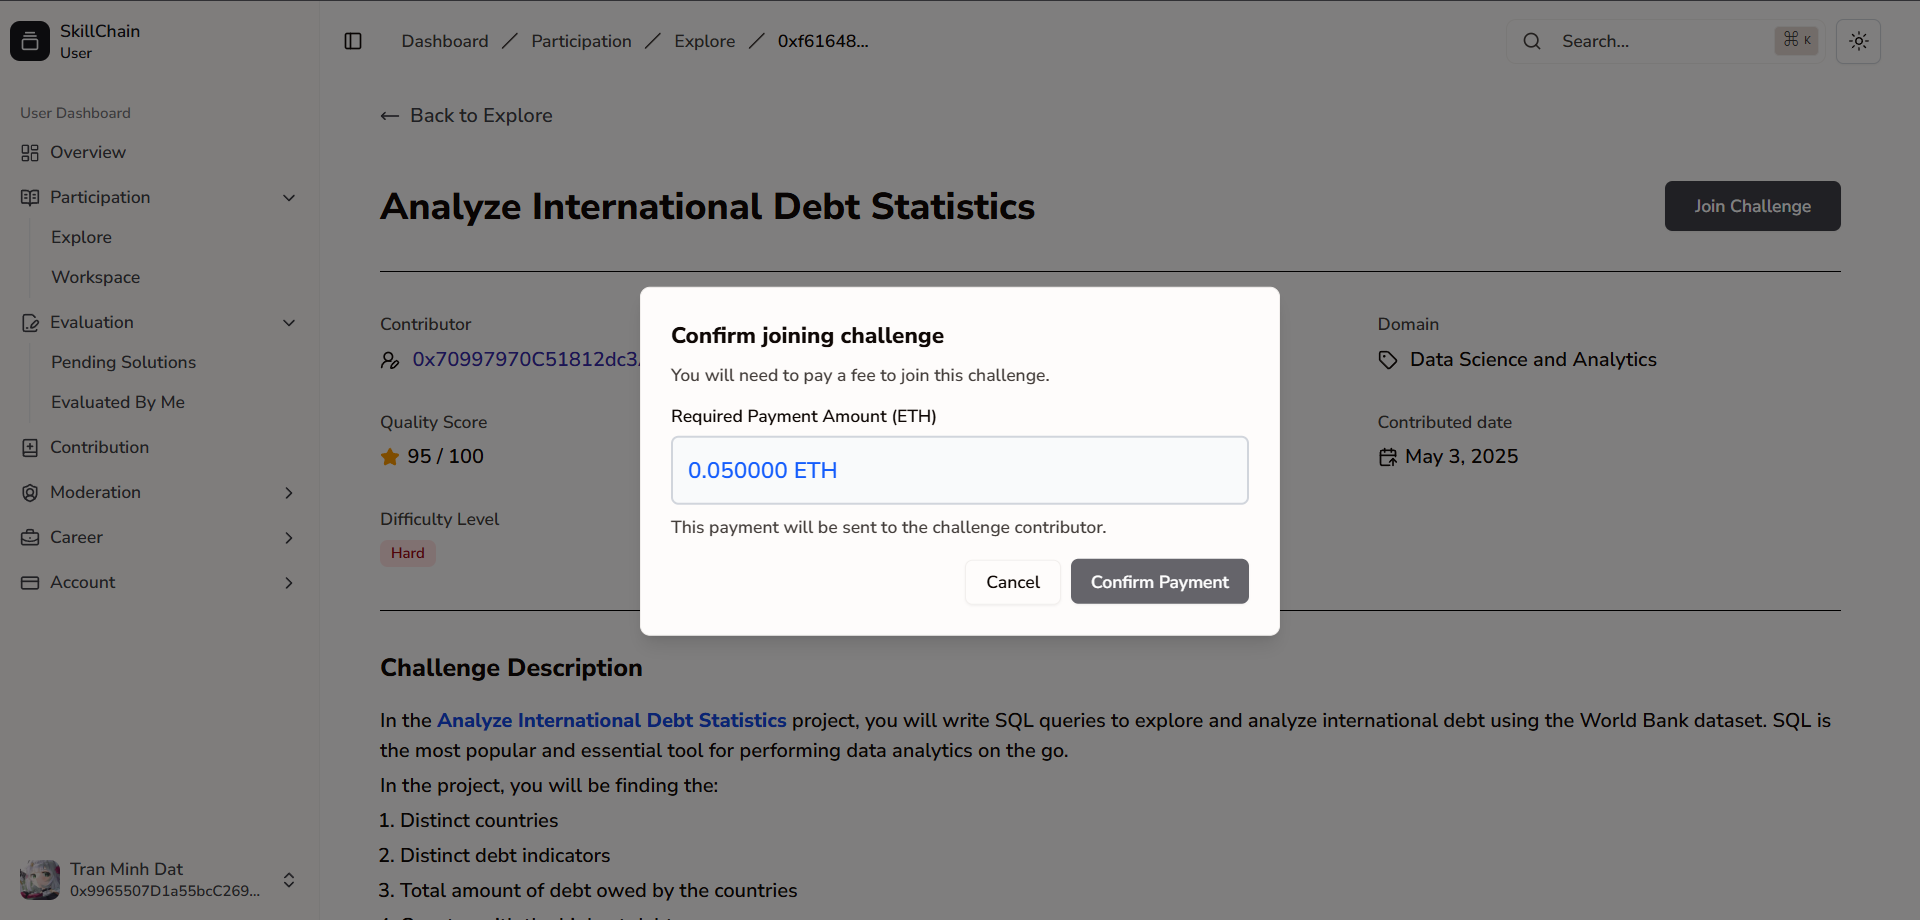
\includegraphics[width=0.99\textwidth, frame]{ui/join-challenge-payment-dialog.png}
  \caption{Xác nhận trả phí tham gia thử thách}
  \label{fig:join-challenge-payment-dialog}
\end{figure}

Sau khi tham gia thành công, người dùng truy cập \textbf{Participation} $\rightarrow$ \textbf{Workspace} để xem các thử thách đã và đang tham gia.  
Tại đây, người dùng có thể bắt đầu xây dựng giải pháp. Hệ thống cho phép lưu tạm giải pháp nhiều lần trước khi nộp chính thức.

\begin{figure}[H]
  \centering
  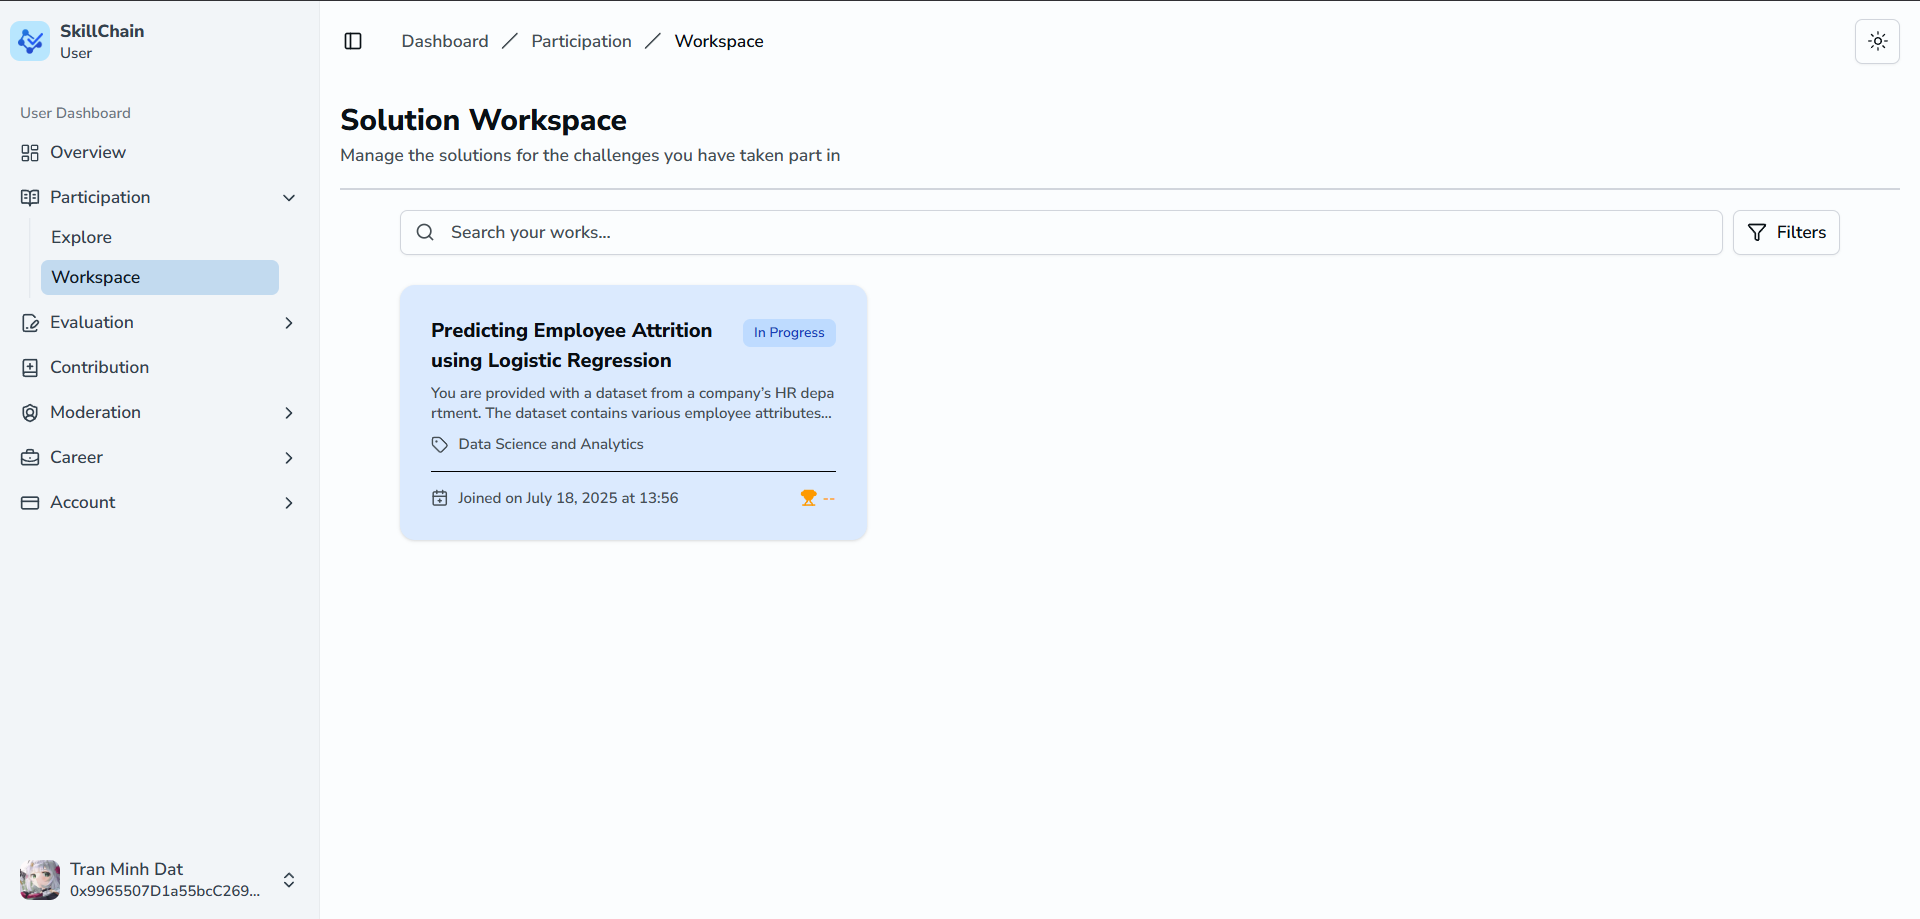
\includegraphics[width=0.99\textwidth, frame]{ui/workspace-challenge-page.png}
  \caption{Trang danh sách thử thách đã tham gia}
  \label{fig:workspace-challenge-page}
\end{figure}

\begin{figure}[H]
  \centering
  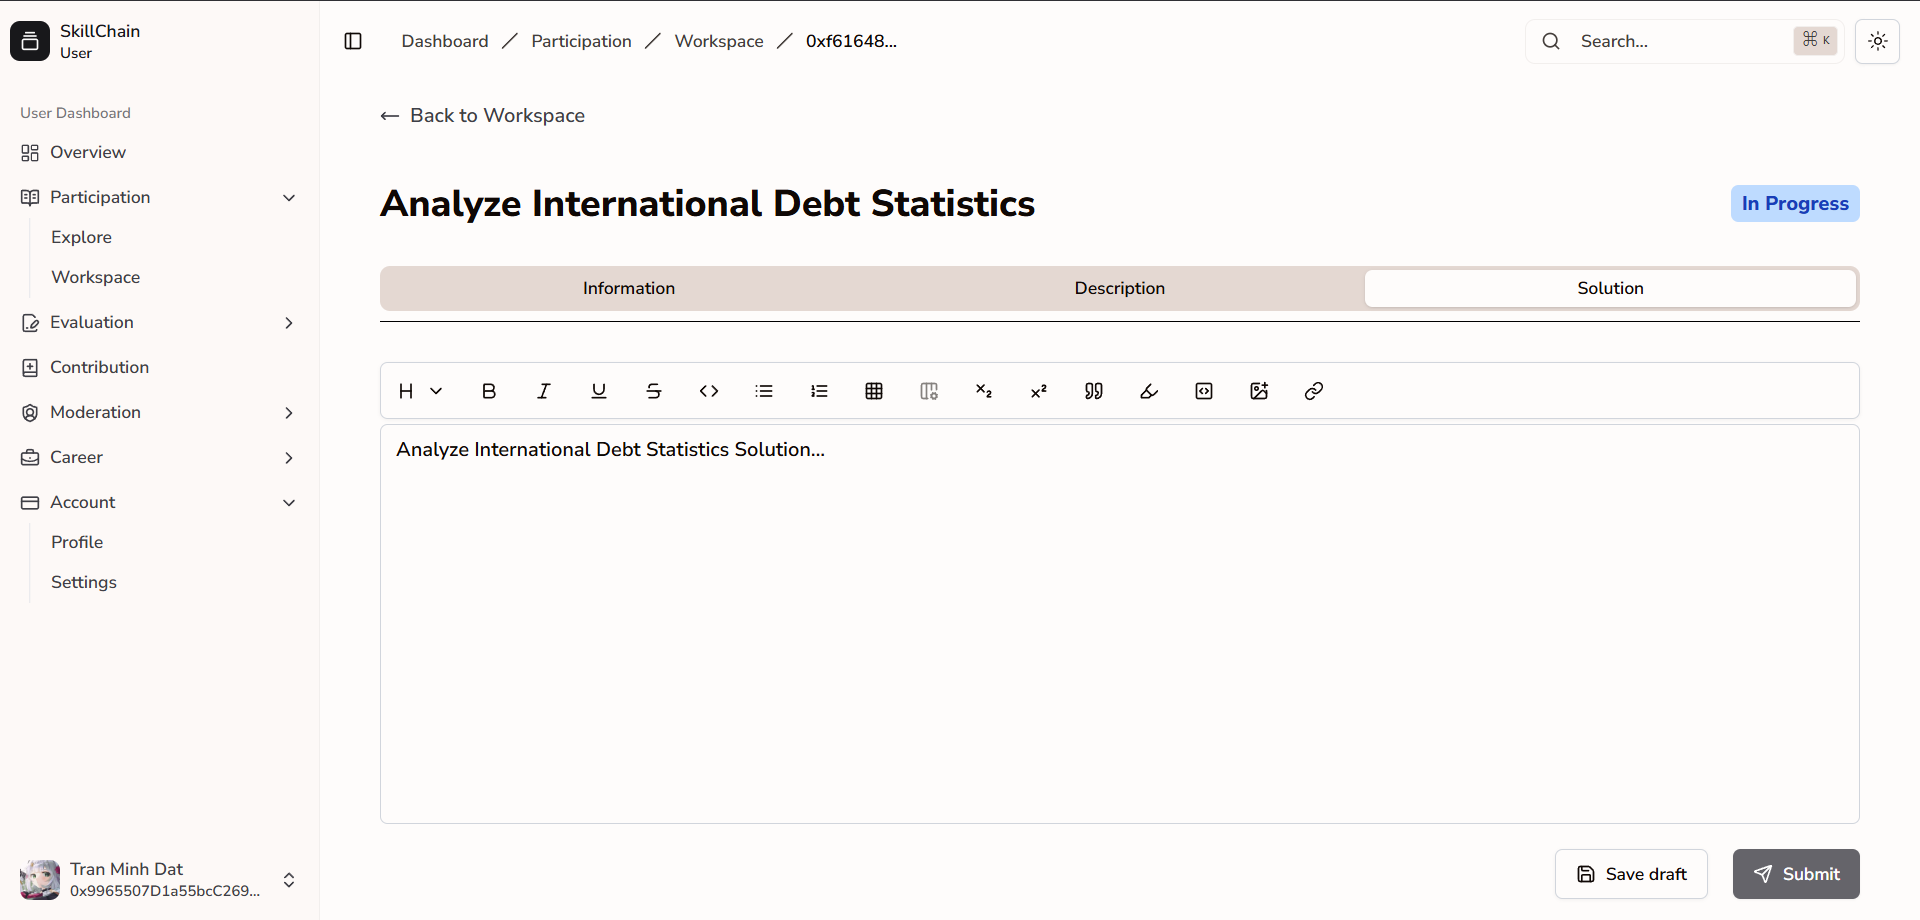
\includegraphics[width=0.99\textwidth, frame]{ui/solution-workspace-page.png}
  \caption{Không gian soạn thảo giải pháp}
  \label{fig:solution-workspace-page}
\end{figure}

Sau khi hoàn thiện giải pháp, người dùng nhấn nút ``Submit'' để nộp bài. Kể từ thời điểm này, nội dung giải pháp sẽ bị khóa và không thể chỉnh sửa.
Khi đã sẵn sàng gửi bài để chấm điểm, người dùng nhấn ``Put Under Review''. Mỗi hành động nộp bài hoặc gửi đánh giá đều yêu cầu xác thực giao dịch thông qua ví tiền điện tử.

\begin{figure}[H]
  \centering
  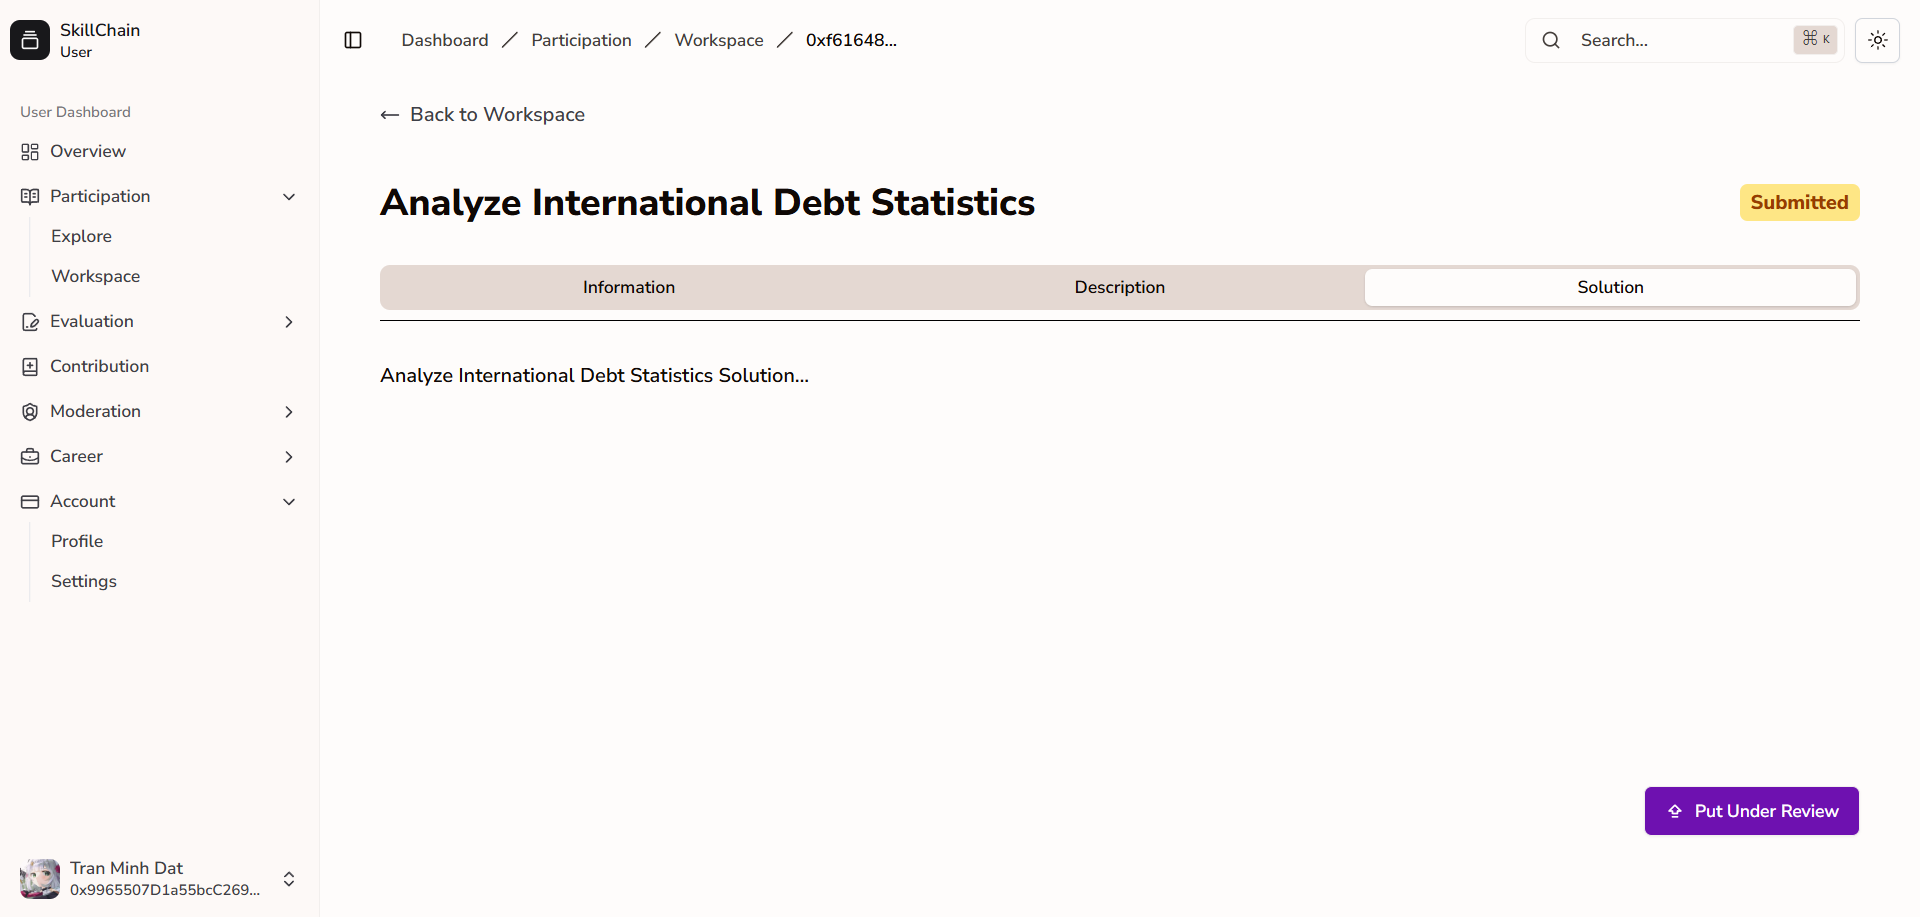
\includegraphics[width=0.99\textwidth, frame]{ui/submitted-solution-page.png}
  \caption{Giải pháp đã được nộp}
  \label{fig:submitted-solution-page}
\end{figure}

\subsection{Đánh giá giải pháp}

\subsubsection{Xem giải pháp đang chờ đánh giá}

Để xem danh sách các giải pháp đang chờ đánh giá, người dùng truy cập \textbf{Evaluation} $\rightarrow$ \textbf{Pending Solution}.  
Tại đây, hệ thống hiển thị các giải pháp đang chờ đánh giá, bao gồm tên người nộp giải, số lượng người đánh giá đã tham gia.  
Tuy nhiên, nội dung chi tiết của giải pháp sẽ chưa được hiển thị ở giai đoạn này.

\begin{figure}[H]
  \centering
  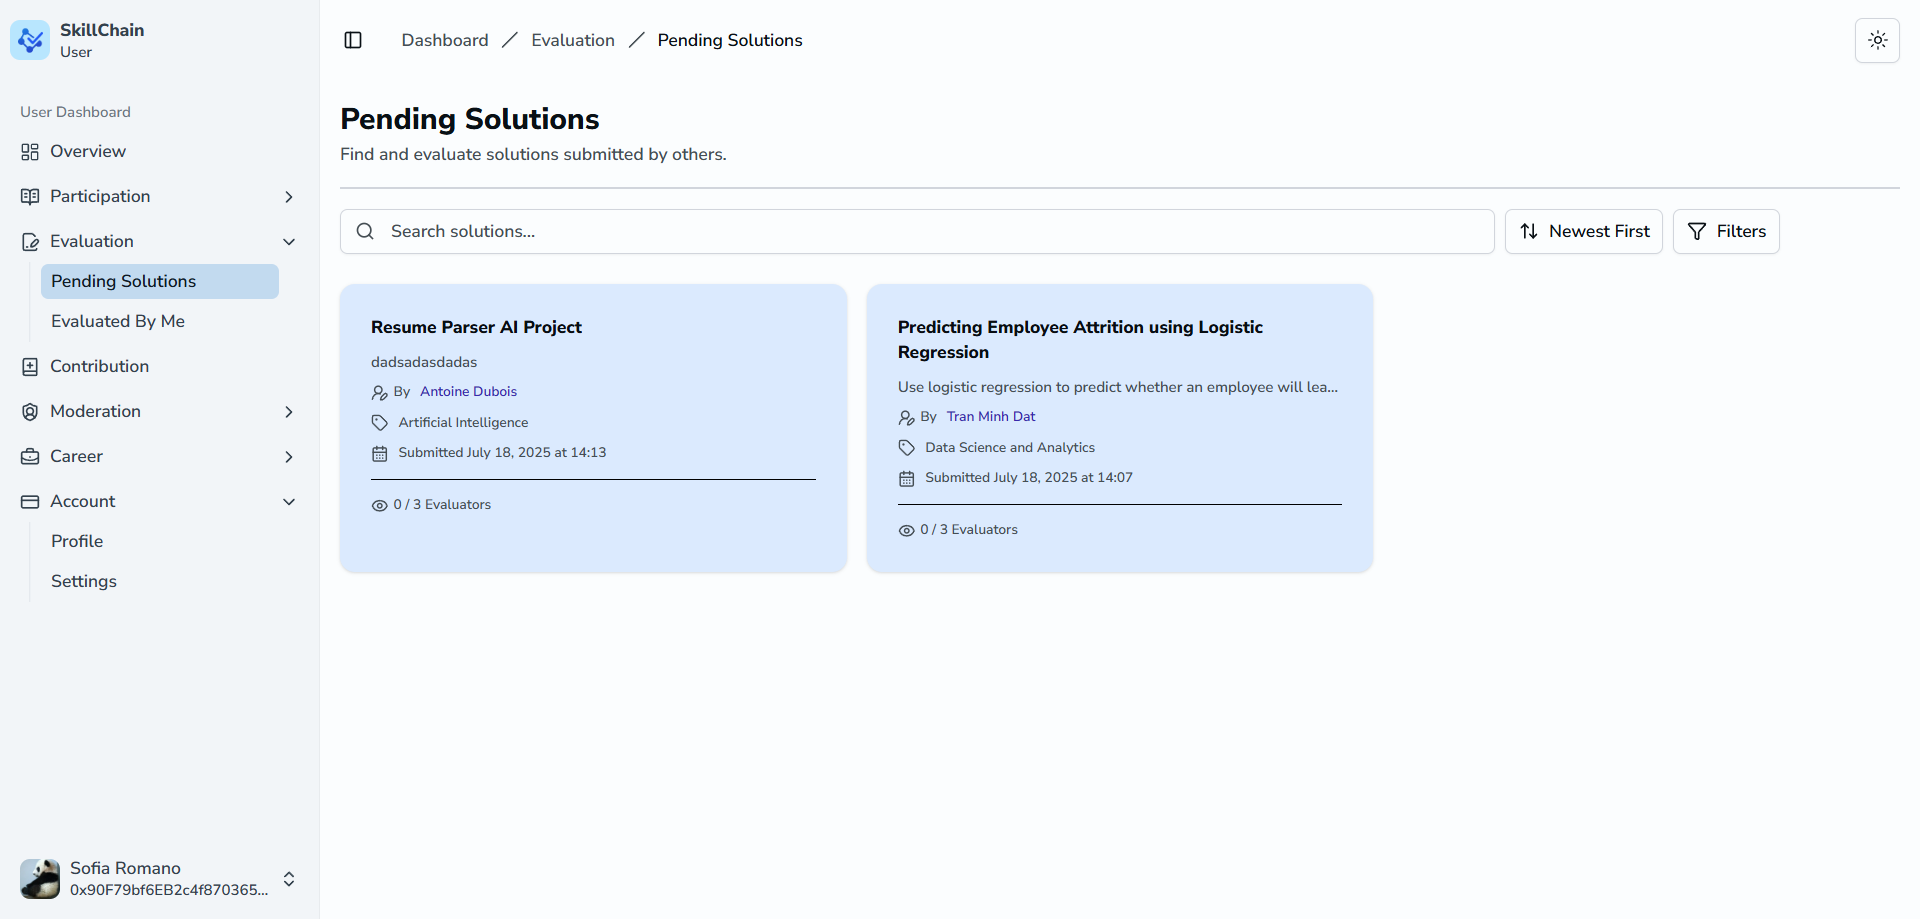
\includegraphics[width=0.99\textwidth, frame]{ui/pending-solution-page.png}
  \caption{Trang danh sách giải pháp đang chờ đánh giá}
  \label{fig:pending-solution-page}
\end{figure}

\subsubsection{Tham gia đánh giá giải pháp}

Khi xem thông tin chi tiết của một giải pháp, người dùng có thể nhấn nút ``Evaluate Solution'' để đăng ký tham gia đánh giá.  
Hệ thống sẽ yêu cầu xác thực giao dịch thông qua ví tiền điện tử để xác nhận quyền đánh giá.
Nếu người dùng không đủ chỉ số uy tín chuyên môn phù hợp với loại thử thách, hệ thống sẽ hiển thị thông báo lỗi và không cho phép tiếp tục.

\begin{figure}[H]
  \centering
  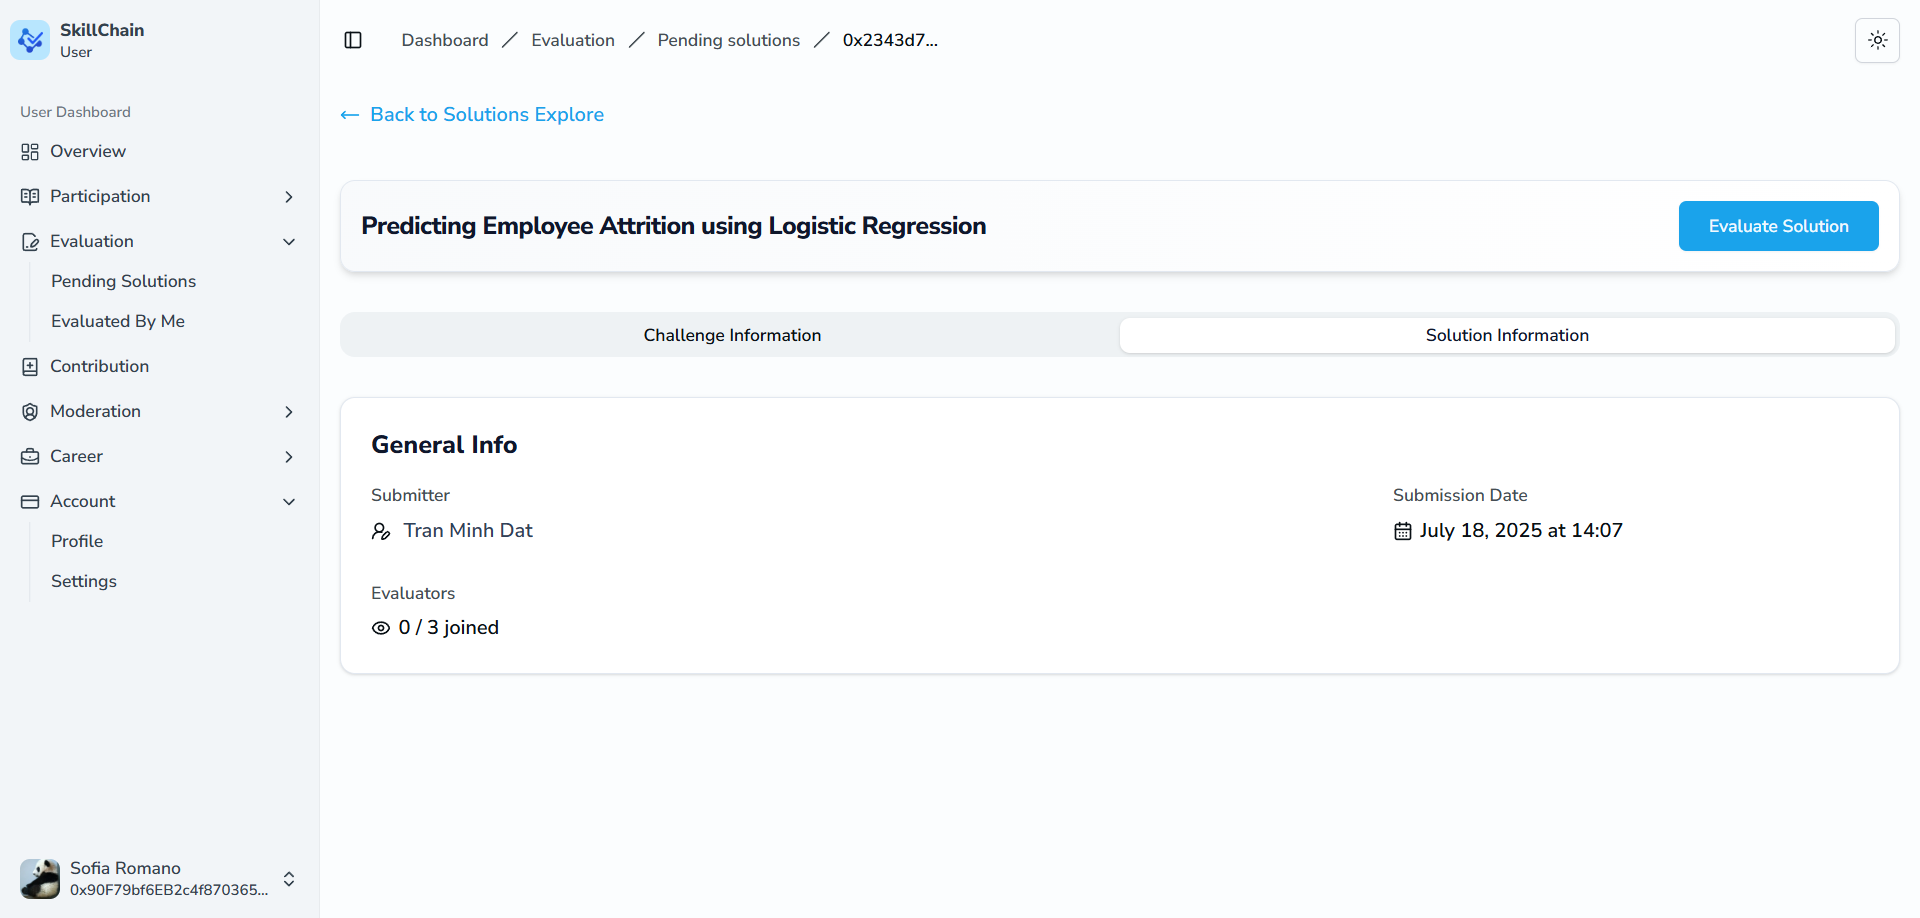
\includegraphics[width=0.99\textwidth, frame]{ui/pending-solution-info-page.png}
  \caption{Thông tin cơ bản của giải pháp đang chờ đánh giá}
  \label{fig:pending-solution-info-page}
\end{figure}

\subsubsection{Thực hiện đánh giá giải pháp}

Sau khi tham gia đánh giá, người dùng truy cập \textbf{Evaluation} $\rightarrow$ \textbf{Evaluated By Me} để xem danh sách các giải pháp mà mình đã hoặc đang đánh giá.  
Tại đây, người đánh giá có thể xem nội dung chi tiết của giải pháp và tiến hành chấm điểm.

\begin{figure}[H]
  \centering
  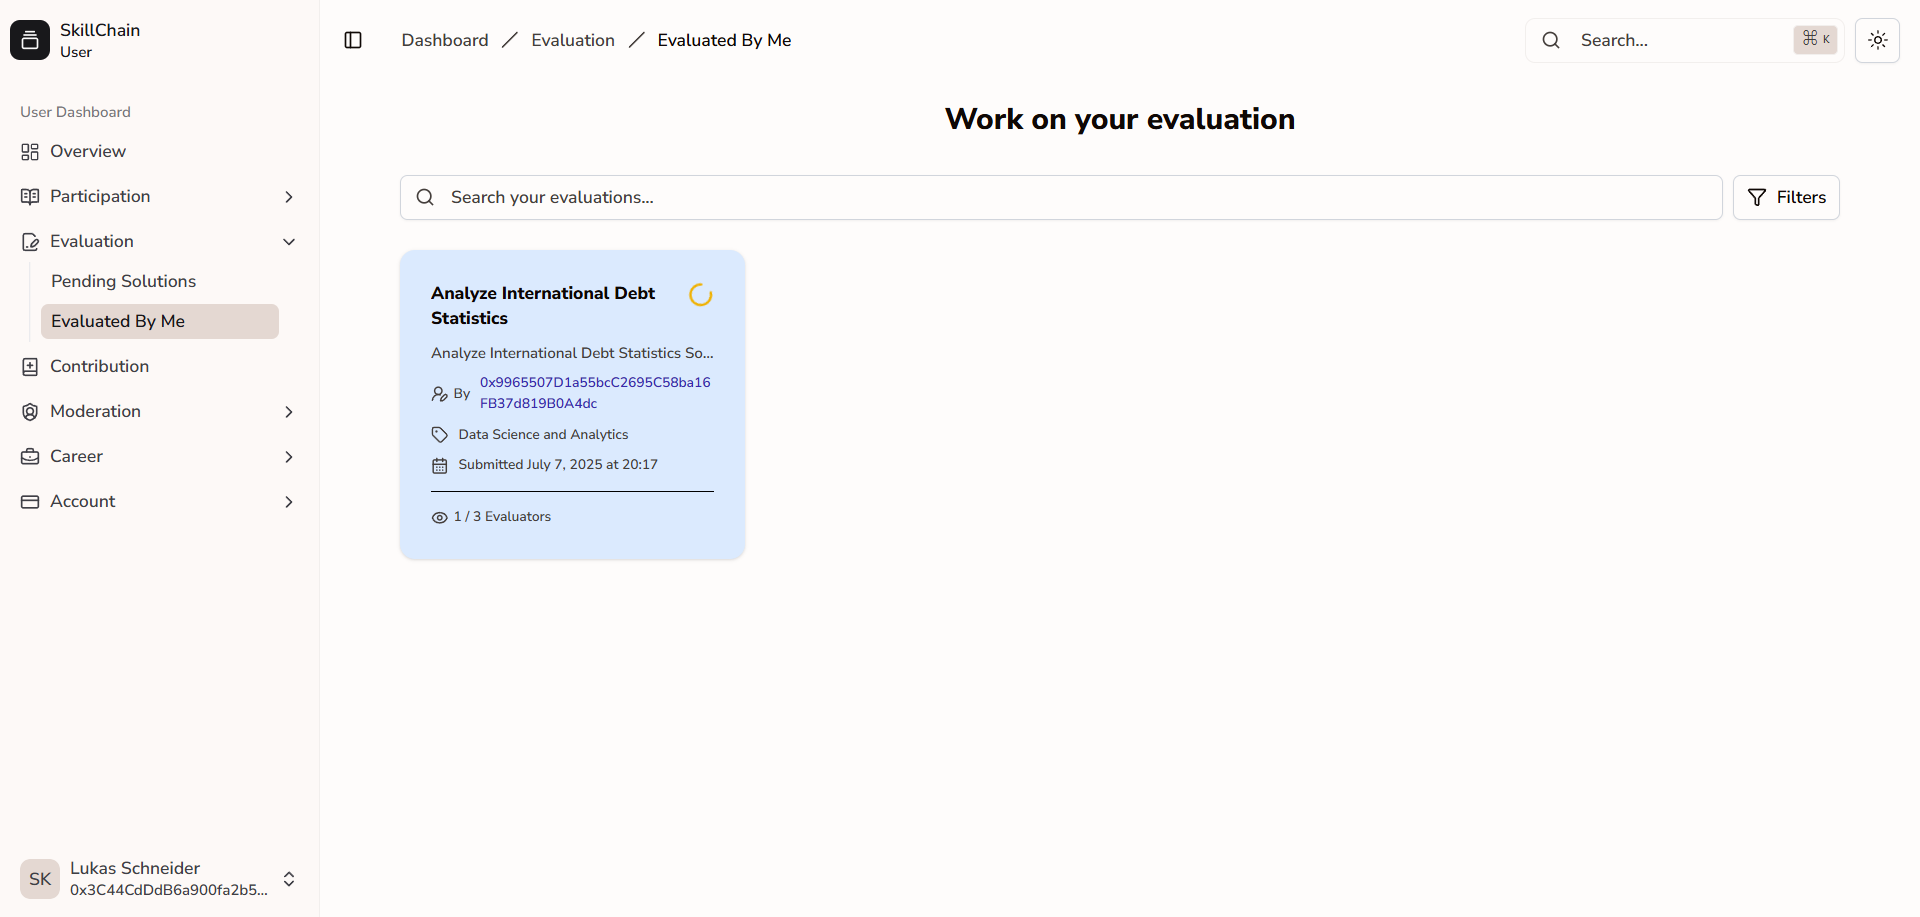
\includegraphics[width=0.99\textwidth, frame]{ui/evaluated-by-me-page.png}
  \caption{Trang danh sách giải pháp đã và đang đánh giá}
  \label{fig:evaluated-by-me-page}
\end{figure}

Người dùng thực hiện đánh giá bằng cách điền nội dung nhận xét, chấm điểm theo thang điểm quy định và nhấn ``Submit'' để nộp kết quả.  
Sau khi gửi đi, kết quả đánh giá sẽ được khóa và không thể chỉnh sửa.

\begin{figure}[H]
  \centering
  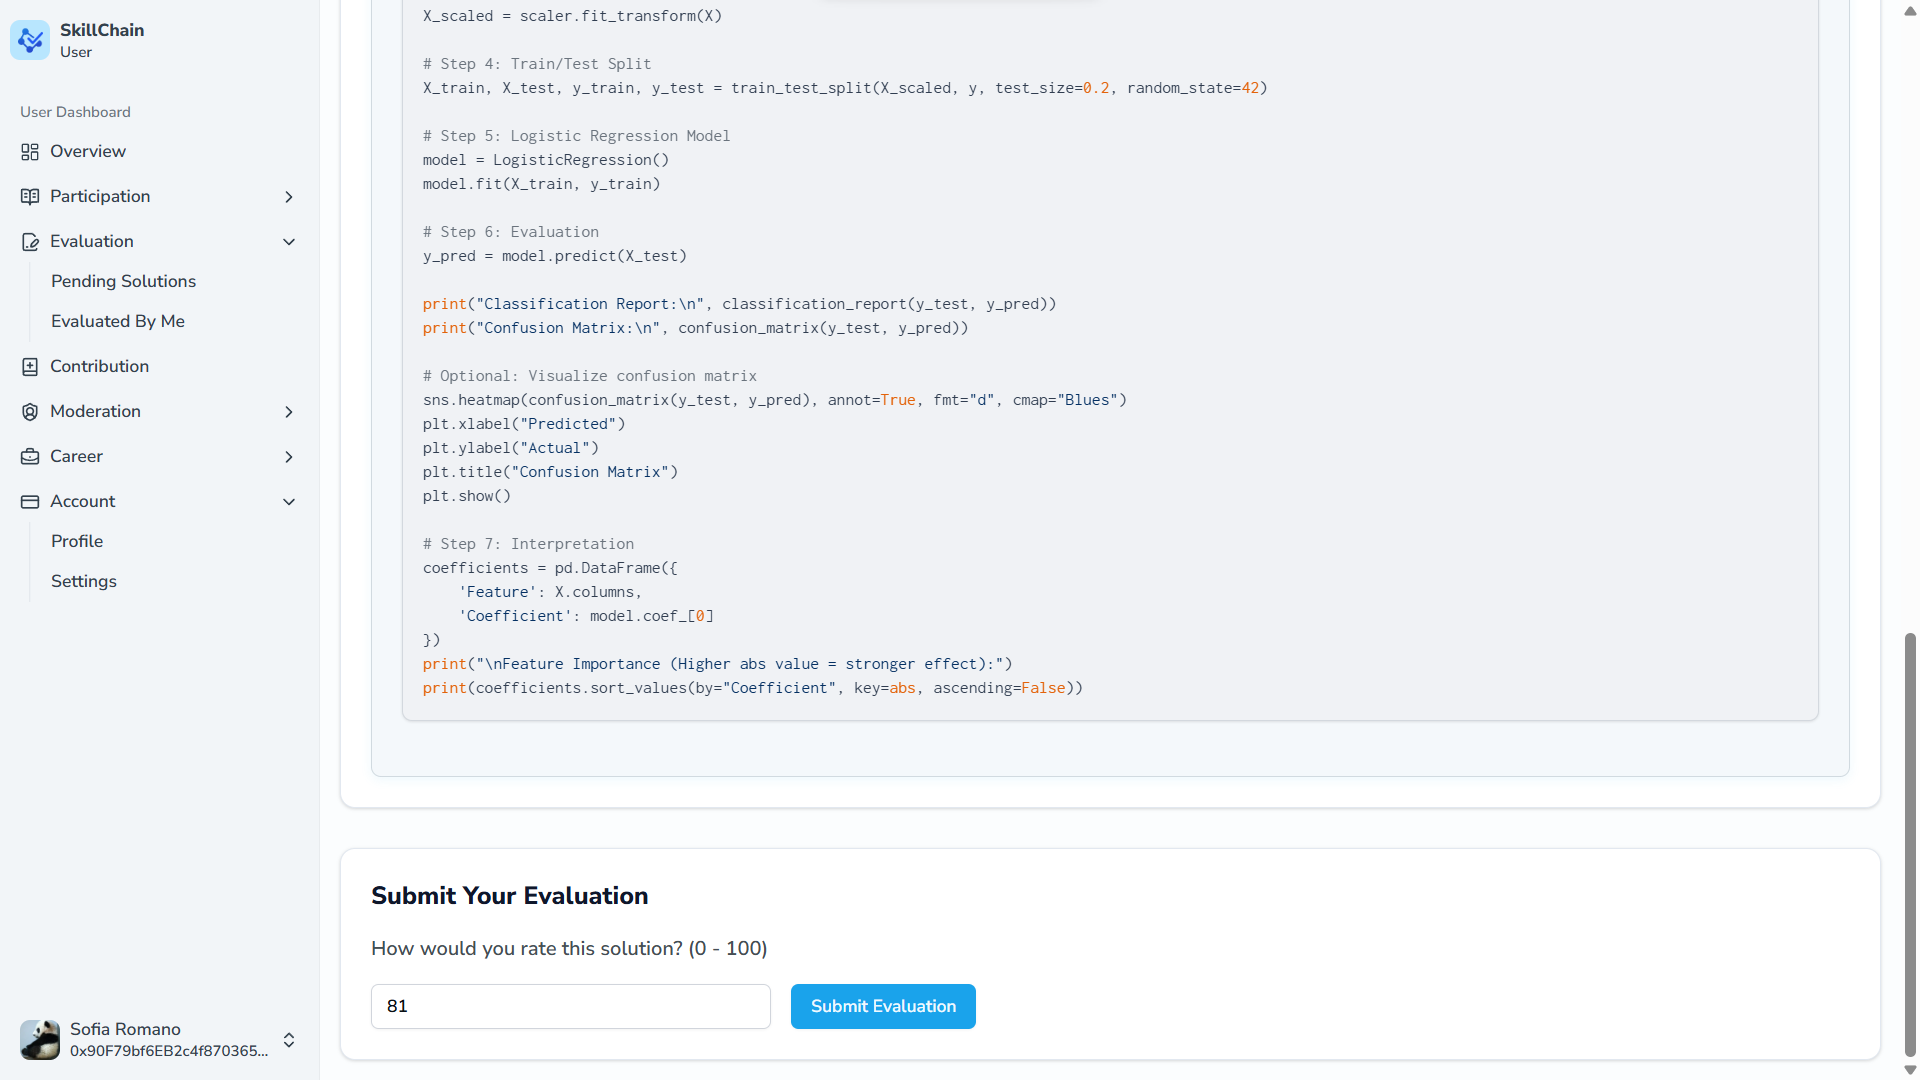
\includegraphics[width=0.99\textwidth, frame]{ui/evaluate-solution-page.png}
  \caption{Trang thực hiện đánh giá giải pháp}
  \label{fig:evaluate-solution-page}
\end{figure}

Sau khi quá trình đánh giá hoàn tất, hệ thống sẽ công khai kết quả phiên đánh giá cho cả người giải và các người đánh giá cũng như cập nhật số người hoàn thành thử thách. 

\begin{figure}[H]
  \centering
  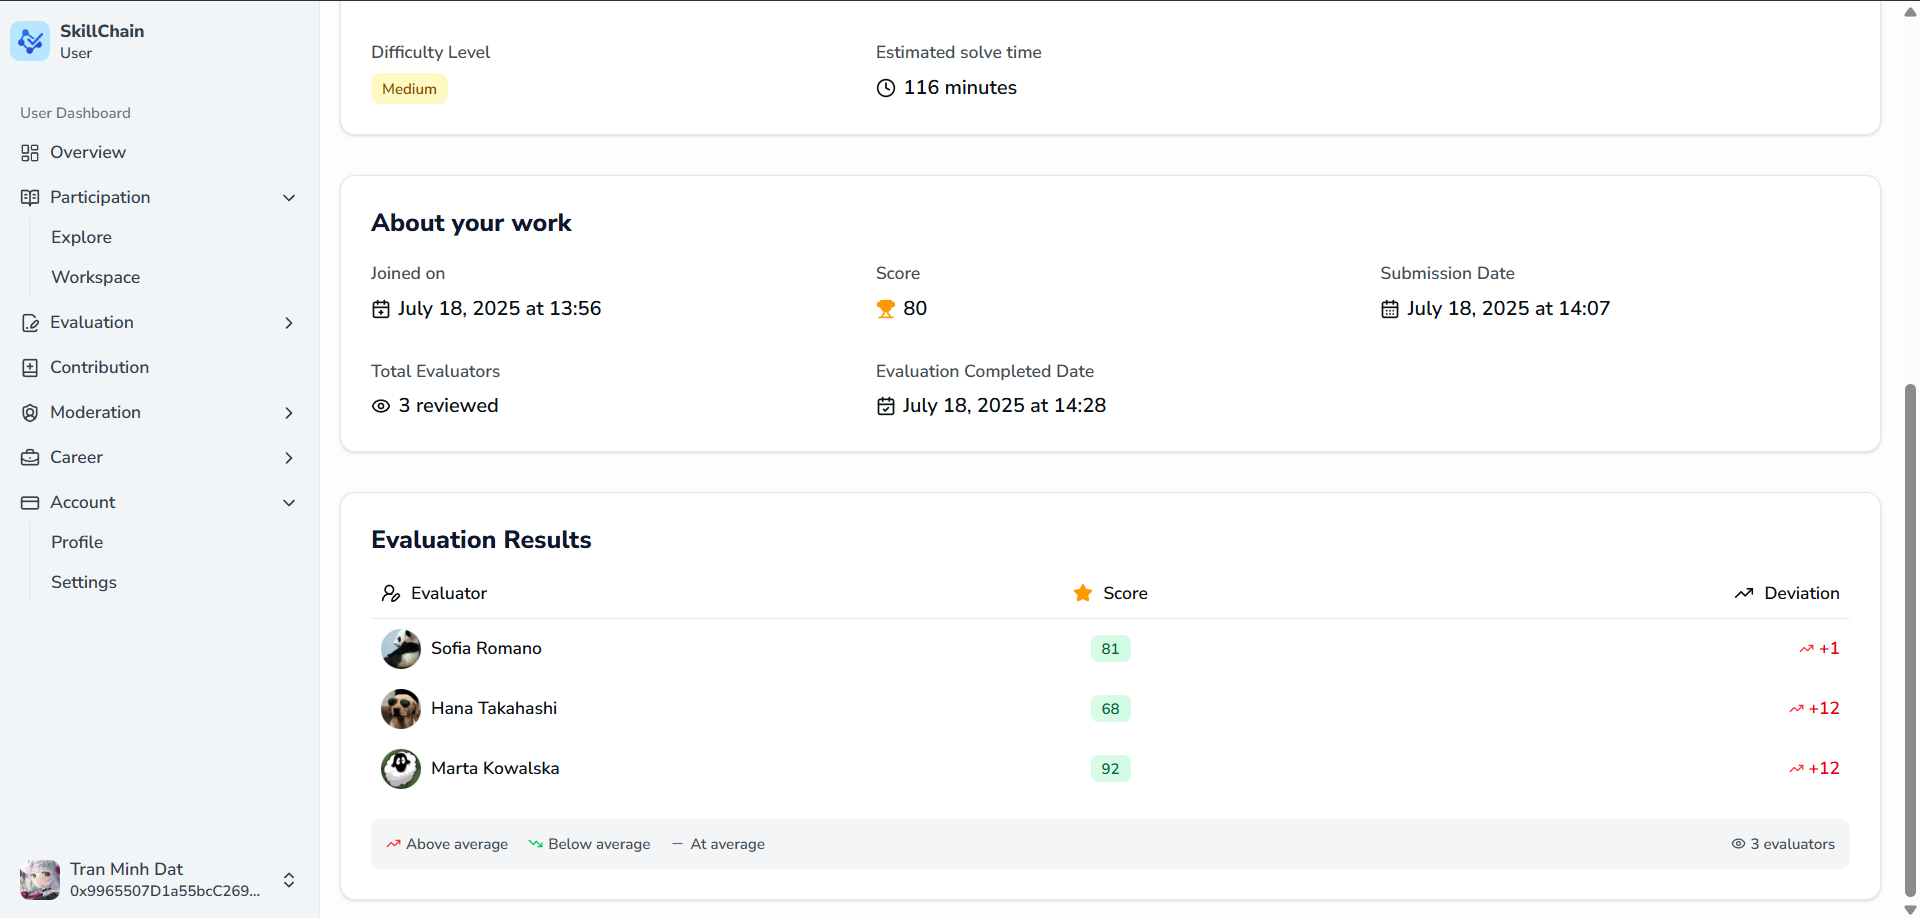
\includegraphics[width=0.99\textwidth, frame]{ui/evaluated-solution-page.png}
  \caption{Giải pháp đã được đánh giá hoàn tất}
  \label{fig:evaluated-solution-page}
\end{figure}

\section{Giao diện tuyển dụng nhân sự}

\subsection{Truy cập không gian nhà tuyển dụng}

Để chuyển sang không gian nhà tuyển dụng, người dùng kết nối ví như thông thường.  
Tại thanh thông tin cá nhân (góc trái bên dưới giao diện), nhấn vào biểu tượng tài khoản và chọn tùy chọn ``Switch to Recruiter''.  
Hệ thống sẽ tự động điều hướng sang không gian làm việc dành riêng cho nhà tuyển dụng.

\begin{figure}[H]
  \centering
  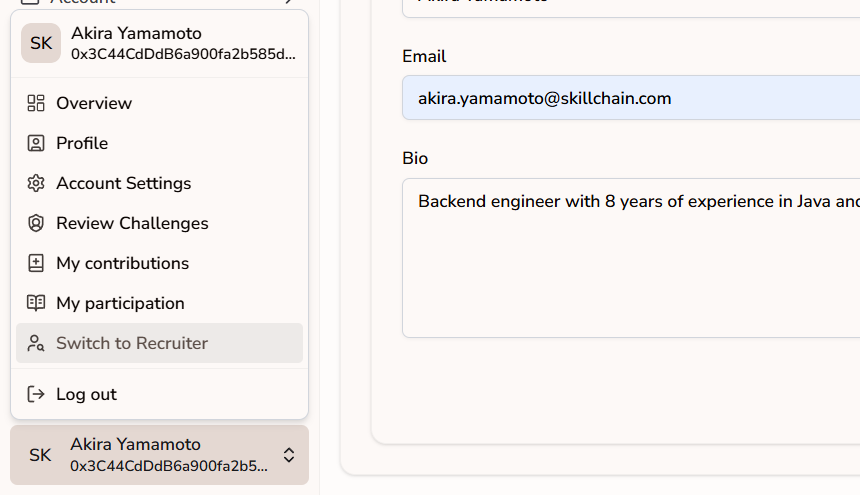
\includegraphics[width=0.99\textwidth, frame]{ui/access-recruiter-space.png}
  \caption{Truy cập không gian nhà tuyển dụng}
  \label{fig:access-recruiter-space}
\end{figure}

\subsection{Tài khoản nhà tuyển dụng}

Tại không gian nhà tuyển dụng, người dùng truy cập tab \textbf{Account} để quản lý hồ sơ cá nhân, thông tin công ty, cũng như thiết lập cấu hình liên quan đến quá trình tuyển dụng.

\subsubsection{Đăng ký trở thành nhà tuyển dụng}

Để sử dụng tính năng tuyển dụng, hệ thống yêu cầu người dùng ký gửi tối thiểu \textbf{1 ETH}.  
Để thực hiện, nhà tuyển dụng truy cập tab \textbf{Account Settings}, nhập số ETH muốn gửi tại mục ``Recruiter Budget'' và nhấn nút ``Deposit''.  
Sau đó, xác nhận giao dịch thông qua ví tiền điện tử.  
Các chi phí phát sinh trong quá trình tuyển dụng sẽ tự động được khấu trừ từ khoản ký gửi này.

\begin{figure}[H]
  \centering
  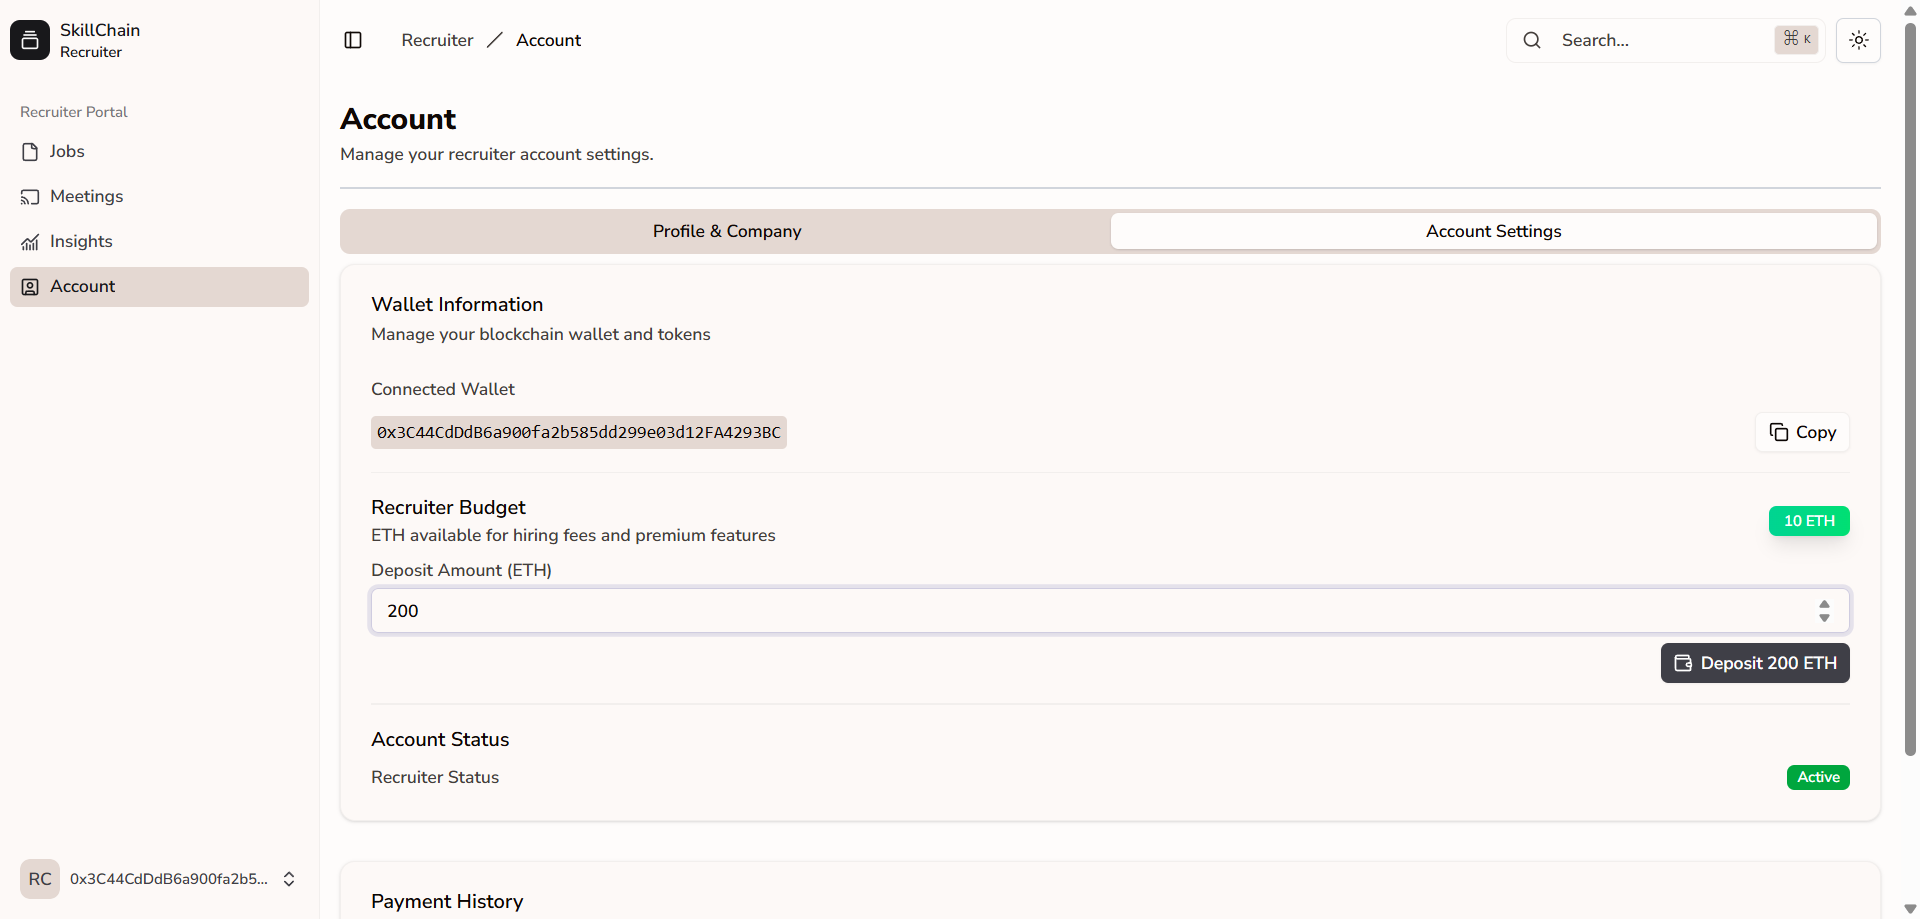
\includegraphics[width=0.99\textwidth, frame]{ui/recruiter-account-settings-page.png}
  \caption{Trang thiết lập tài khoản nhà tuyển dụng}
  \label{fig:recruiter-account-settings-page}
\end{figure}

\subsubsection{Quản lý hồ sơ nhà tuyển dụng}

Tại tab \textbf{Profile \& Company}, nhà tuyển dụng có thể đăng ký hoặc cập nhật hồ sơ cá nhân và thông tin công ty.  
Trong lần truy cập đầu tiên, hệ thống yêu cầu xác thực giao dịch qua ví điện tử để hoàn tất đăng ký.

\begin{figure}[H]
  \centering
  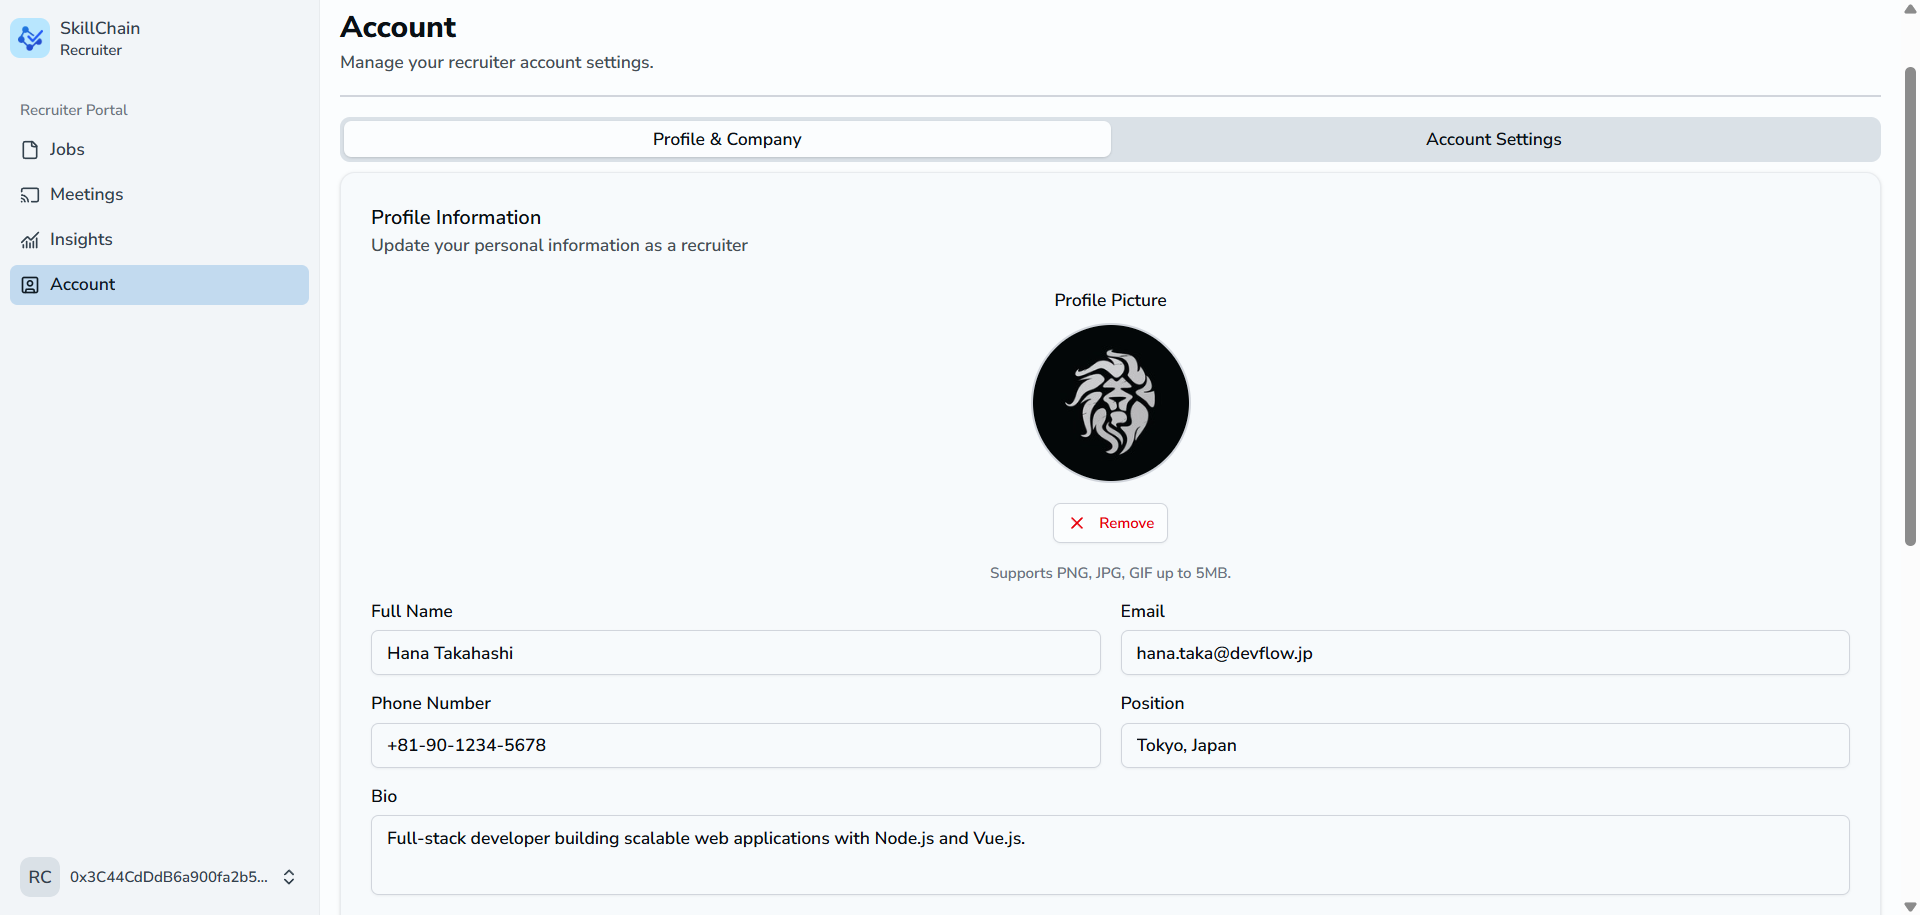
\includegraphics[width=0.99\textwidth, frame]{ui/recruiter-personal-profile.png}
  \caption{Hồ sơ cá nhân nhà tuyển dụng}
  \label{fig:recruiter-personal-profile}
\end{figure}

\begin{figure}[H]
  \centering
  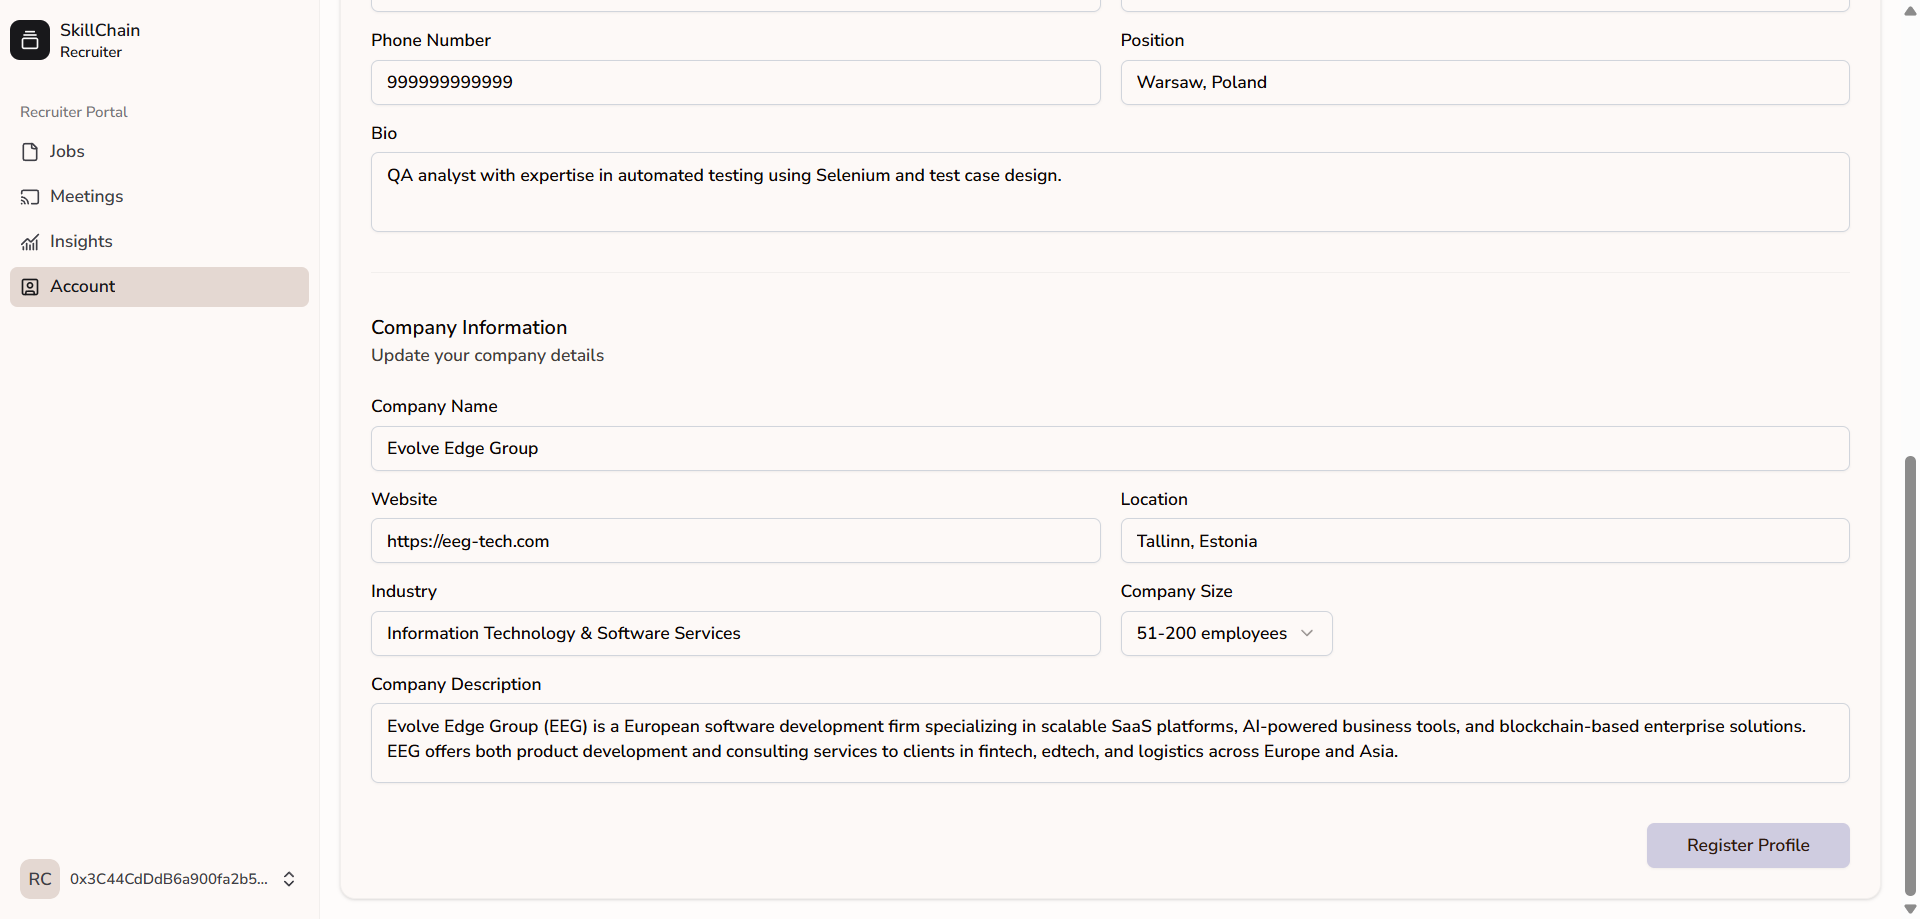
\includegraphics[width=0.99\textwidth, frame]{ui/recruiter-company-profile.png}
  \caption{Thông tin công ty của nhà tuyển dụng}
  \label{fig:recruiter-company-profile}
\end{figure}

\subsection{Quản lý bài đăng}

\subsubsection{Xem danh sách các bài đăng tuyển dụng}

Để xem danh sách các bài đăng tuyển dụng, nhà tuyển dụng truy cập tab \textbf{Jobs}.  
Tại đây, hệ thống hiển thị danh sách các bài đăng đã tạo cùng với thông tin trạng thái, số lượng ứng viên đã ứng tuyển và các hành động có thể thực hiện.

\begin{figure}[H]
  \centering
  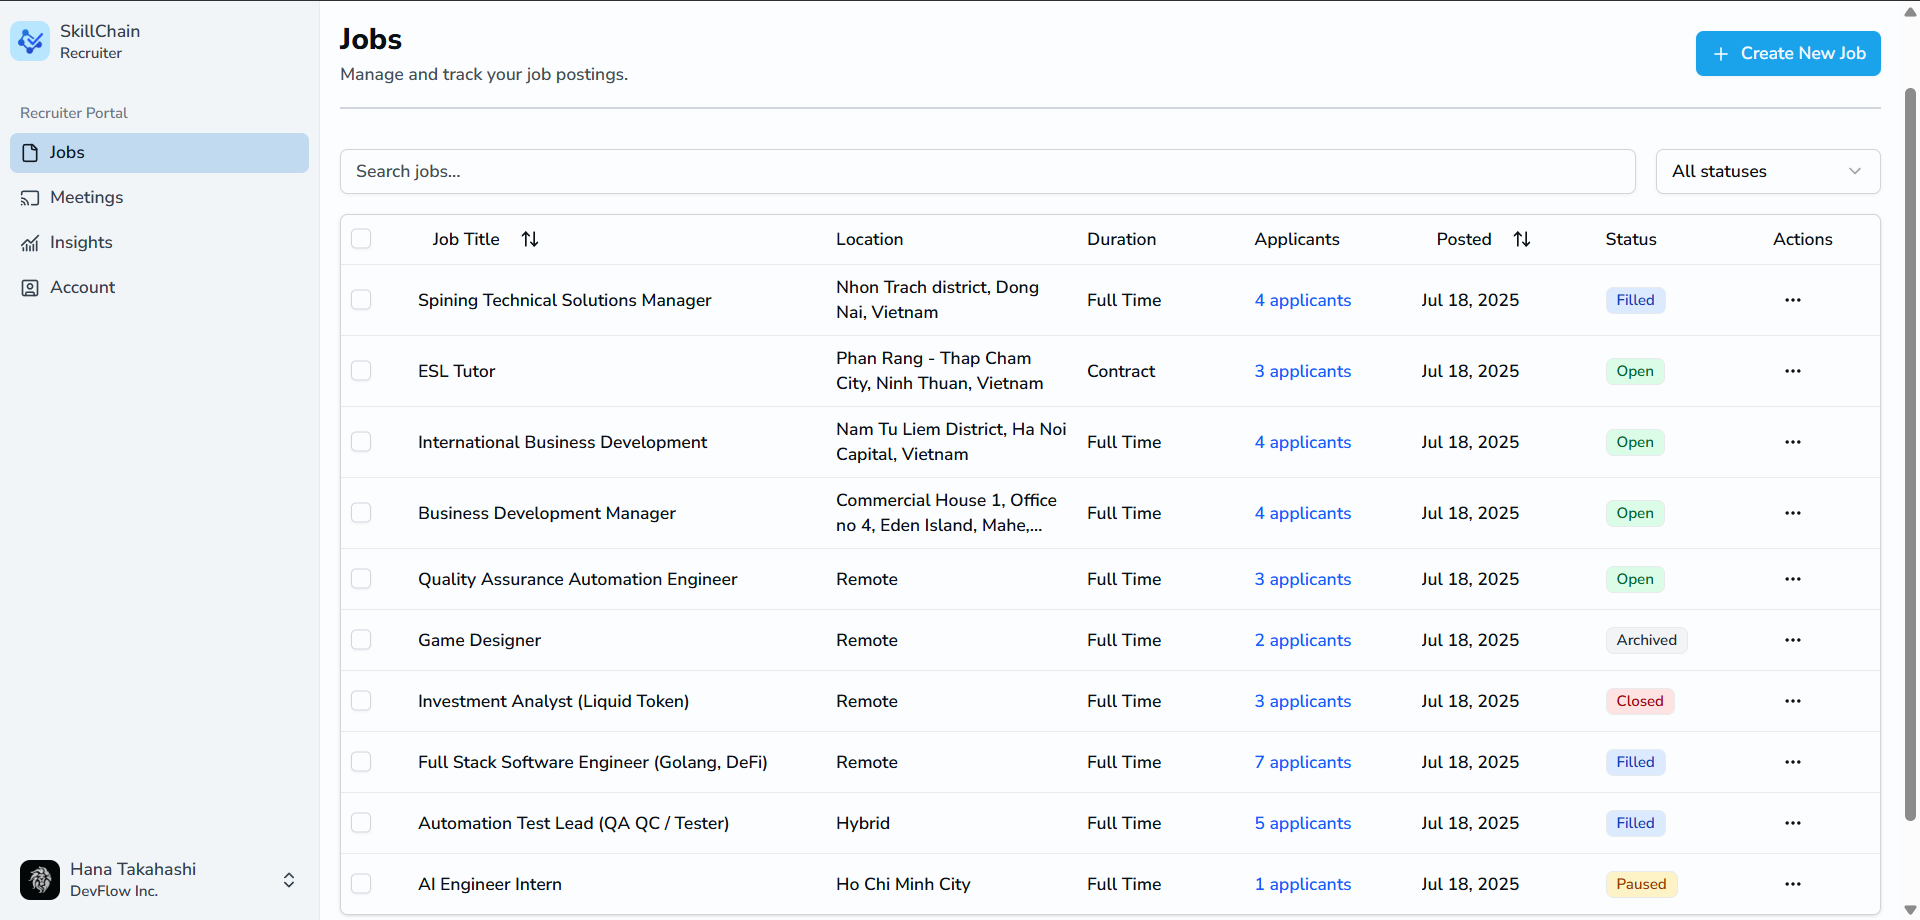
\includegraphics[width=0.99\textwidth, frame]{ui/jobs-page.png}
  \caption{Trang danh sách các bài đăng tuyển dụng}
  \label{fig:jobs-page}
\end{figure}

Để xem chi tiết một bài đăng, nhà tuyển dụng nhấn ``View job'' tại nút ``Actions'' tương ứng.

\begin{figure}[H]
  \centering
  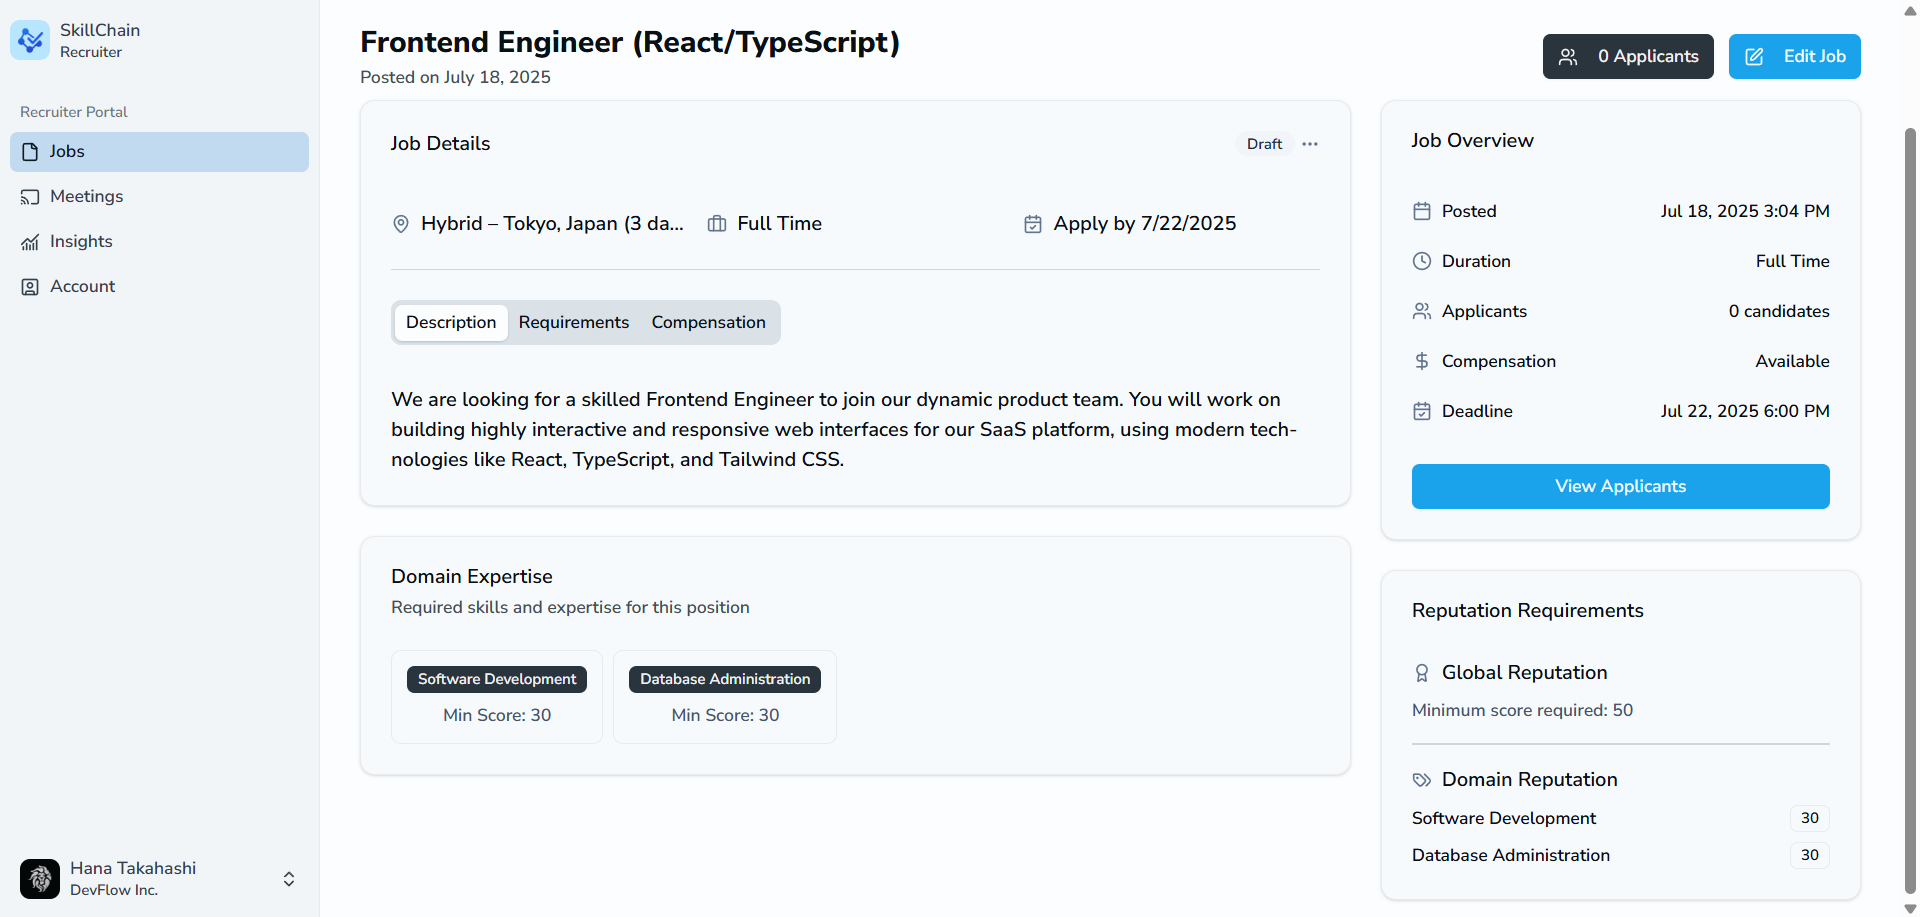
\includegraphics[width=0.99\textwidth, frame]{ui/job-detail-page.png}
  \caption{Trang chi tiết một bài đăng tuyển dụng}
  \label{fig:job-detail-page}
\end{figure}

\subsubsection{Tạo bài đăng tuyển dụng mới}

Để tạo bài đăng mới, nhà tuyển dụng nhấn nút ``Create New Job'' ở góc trên bên phải.  
Tại giao diện tạo bài đăng, nhà tuyển dụng nhập thông tin vị trí công việc, thời hạn đăng bài, cùng với các yêu cầu về uy tín đối với ứng viên.  
Sau khi hoàn tất, nhấn nút ``Create Job'' và xác nhận giao dịch qua ví điện tử để tạo bài đăng ở trạng thái nháp.

\begin{figure}[H]
  \centering
  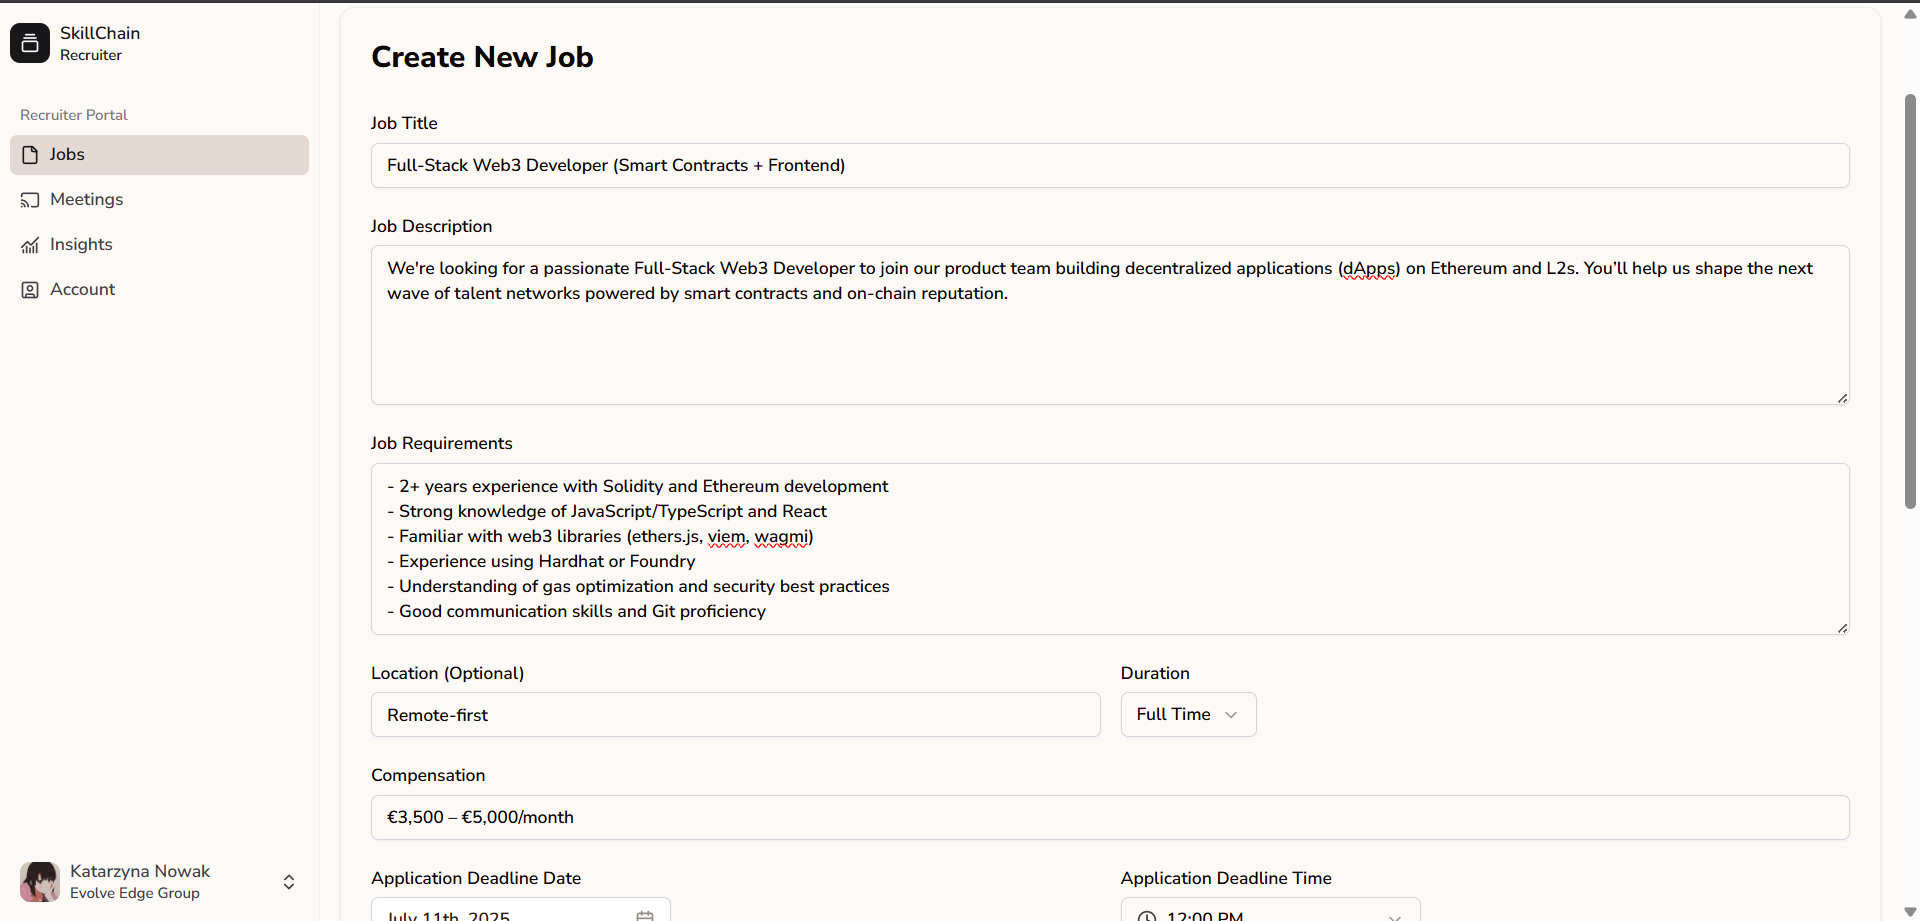
\includegraphics[width=0.99\textwidth, frame]{ui/job-position-info.png}
  \caption{Thông tin về vị trí công việc}
  \label{fig:job-position-info}
\end{figure}

\begin{figure}[H]
  \centering
  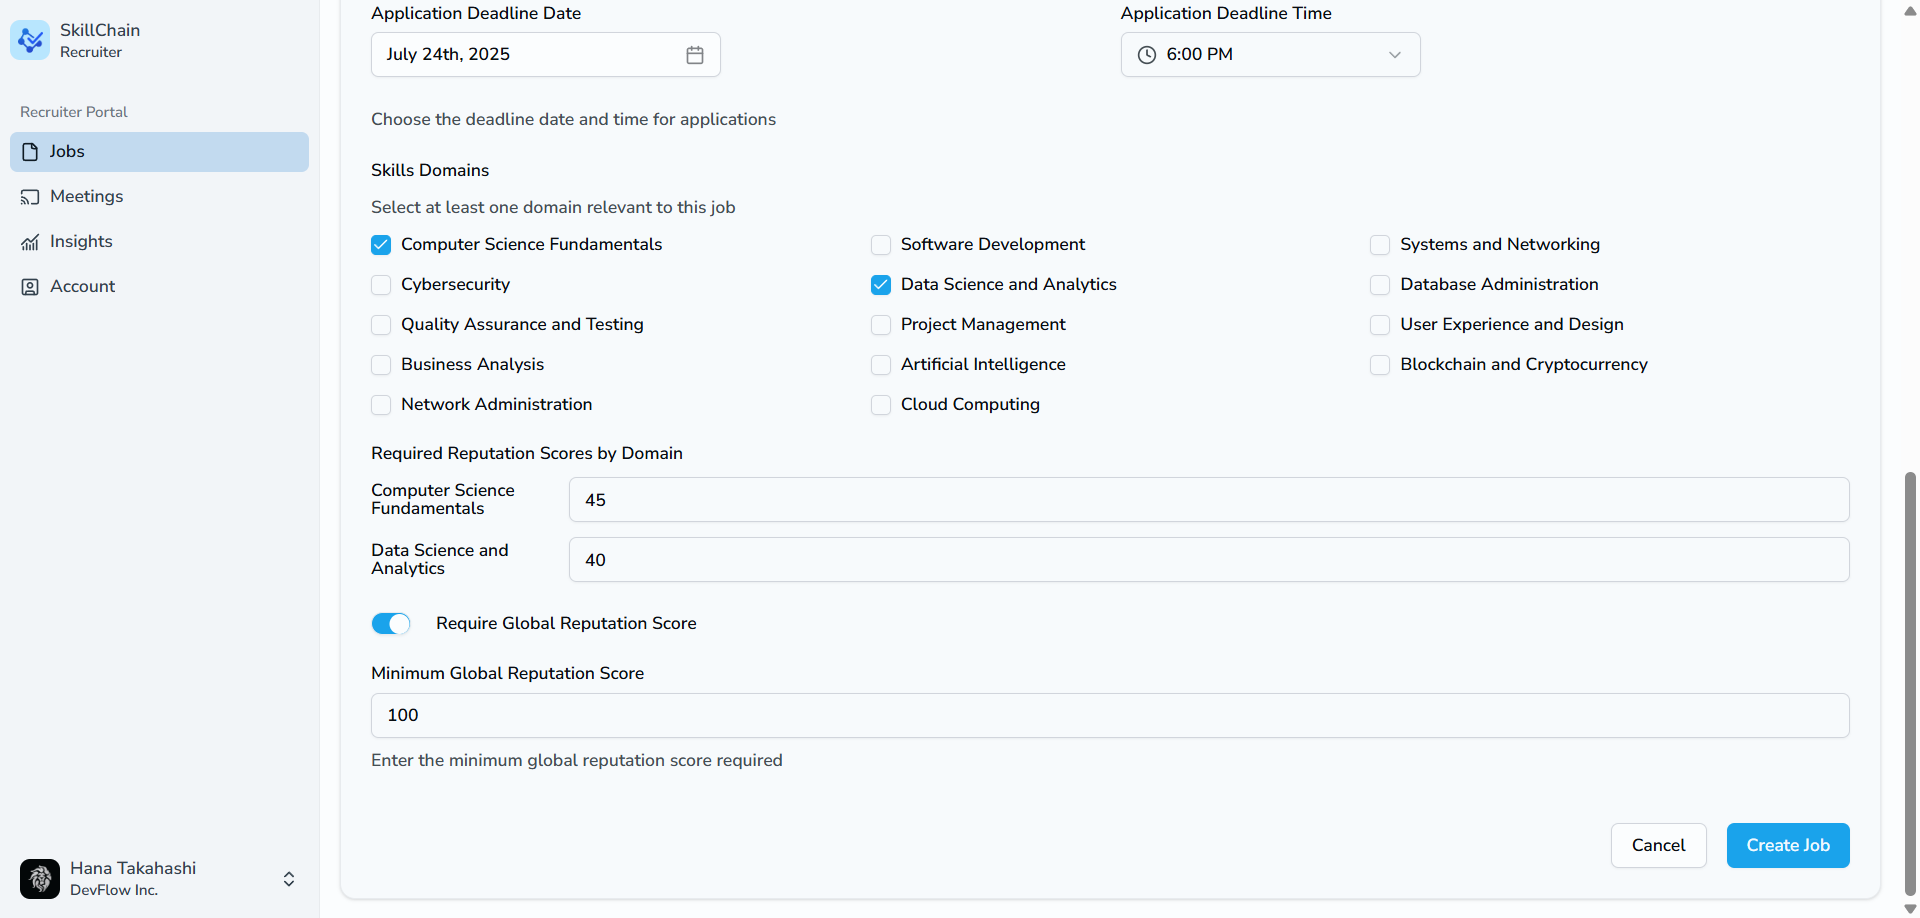
\includegraphics[width=0.99\textwidth, frame]{ui/job-reputation-requirement.png}
  \caption{Yêu cầu uy tín đối với ứng viên}
  \label{fig:job-reputation-requirement}
\end{figure}

\subsubsection{Chỉnh sửa nội dung bài đăng}

Để chỉnh sửa nội dung bài đăng, nhà tuyển dụng có thể thực hiện theo hai cách:
\begin{itemize}
  \item Từ trang chi tiết bài đăng, nhấn ``Edit Job'' ở góc trên bên phải.
  \item Từ danh sách bài đăng, chọn ``Edit job'' tại mục ``Actions''.
\end{itemize}

Hệ thống cho phép chỉnh sửa nội dung trong mọi trạng thái bài đăng mà không phát sinh giao dịch.

\begin{figure}[H]
  \centering
  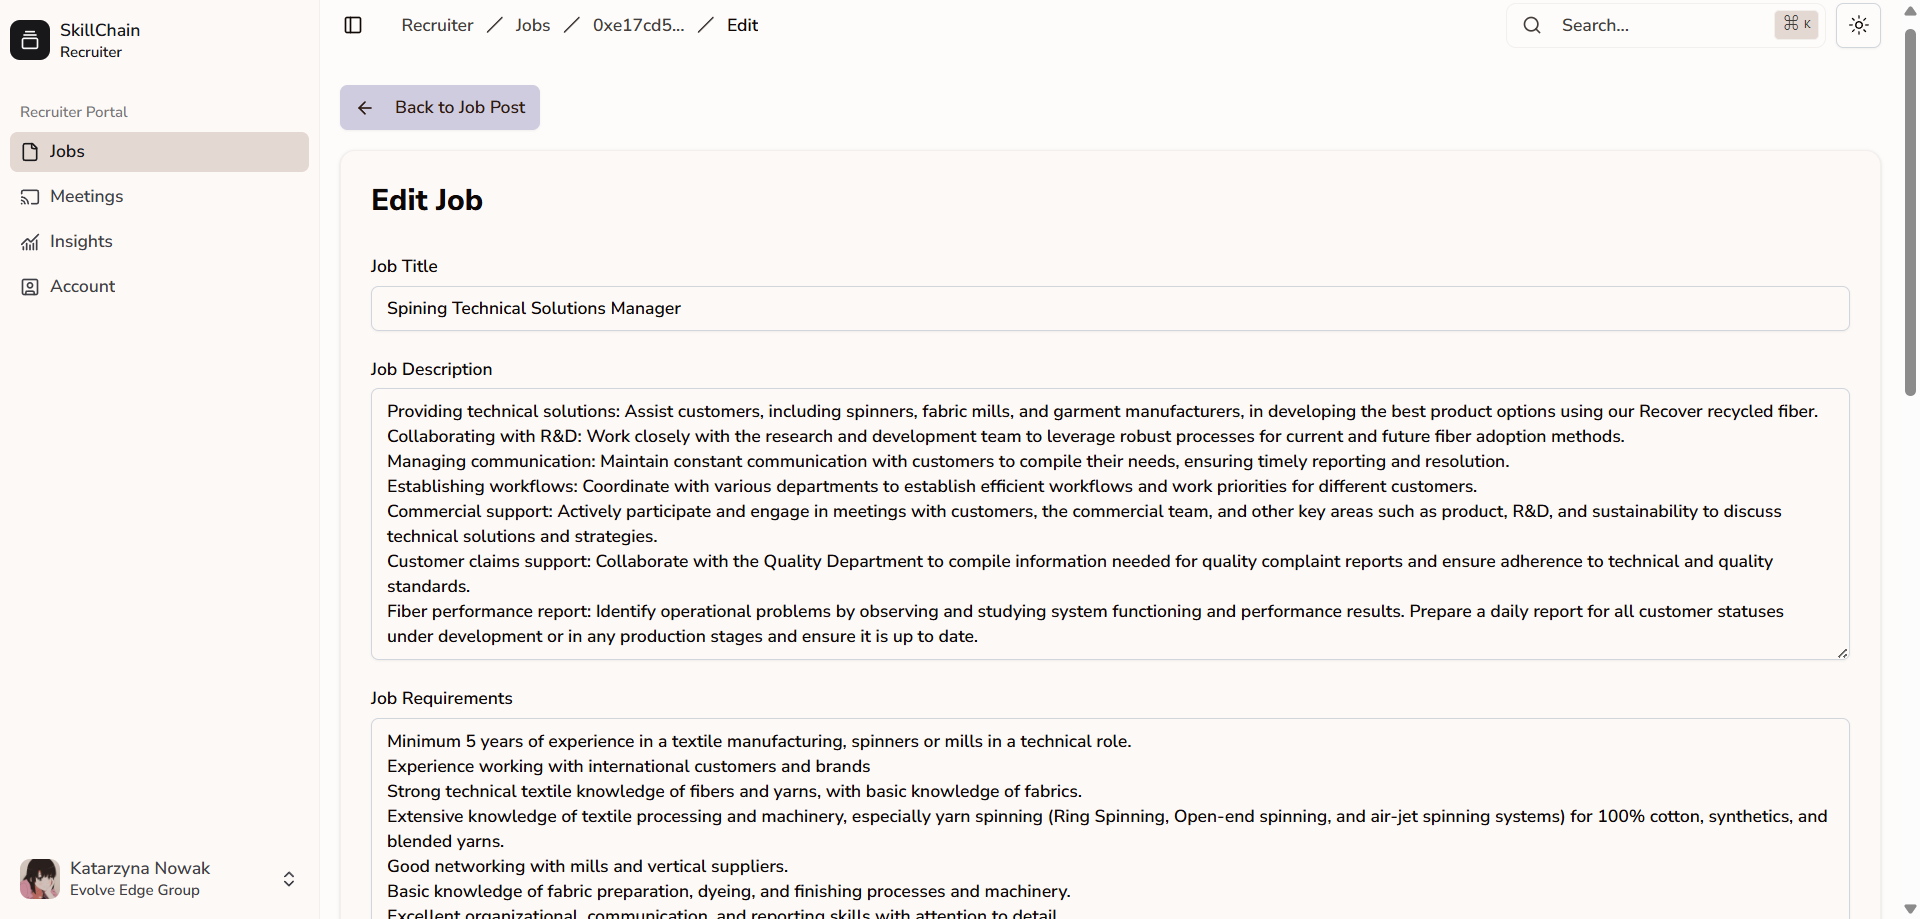
\includegraphics[width=0.99\textwidth, frame]{ui/edit-job-page.png}
  \caption{Trang chỉnh sửa bài đăng tuyển dụng}
  \label{fig:edit-job-page}
\end{figure}

\subsubsection{Chuyển đổi trạng thái bài đăng}

Tại trang chi tiết bài đăng, để thay đổi trạng thái (ví dụ: từ ``nháp'' sang ``đang mở''), nhà tuyển dụng nhấn biểu tượng ba chấm bên cạnh thông tin trạng thái trong phần ``Job Details'' và chọn trạng thái mong muốn.  
Thao tác này yêu cầu xác nhận giao dịch qua ví điện tử.

\subsection{Quản lý thông tin ứng tuyển}

\subsubsection{Xem thông tin ứng tuyển}

Để xem danh sách ứng viên đã ứng tuyển cho một bài đăng, nhà tuyển dụng có thể thực hiện theo hai cách:
\begin{itemize}
  \item Từ trang chi tiết bài đăng, nhấn nút ``View Applicants'' trong phần ``Job Overview''.
  \item Từ danh sách bài đăng, chọn ``View applicants'' tại mục ``Actions'' hoặc nhấn vào liên kết tại cột ``Applicants''.
\end{itemize}

\begin{figure}[H]
  \centering
  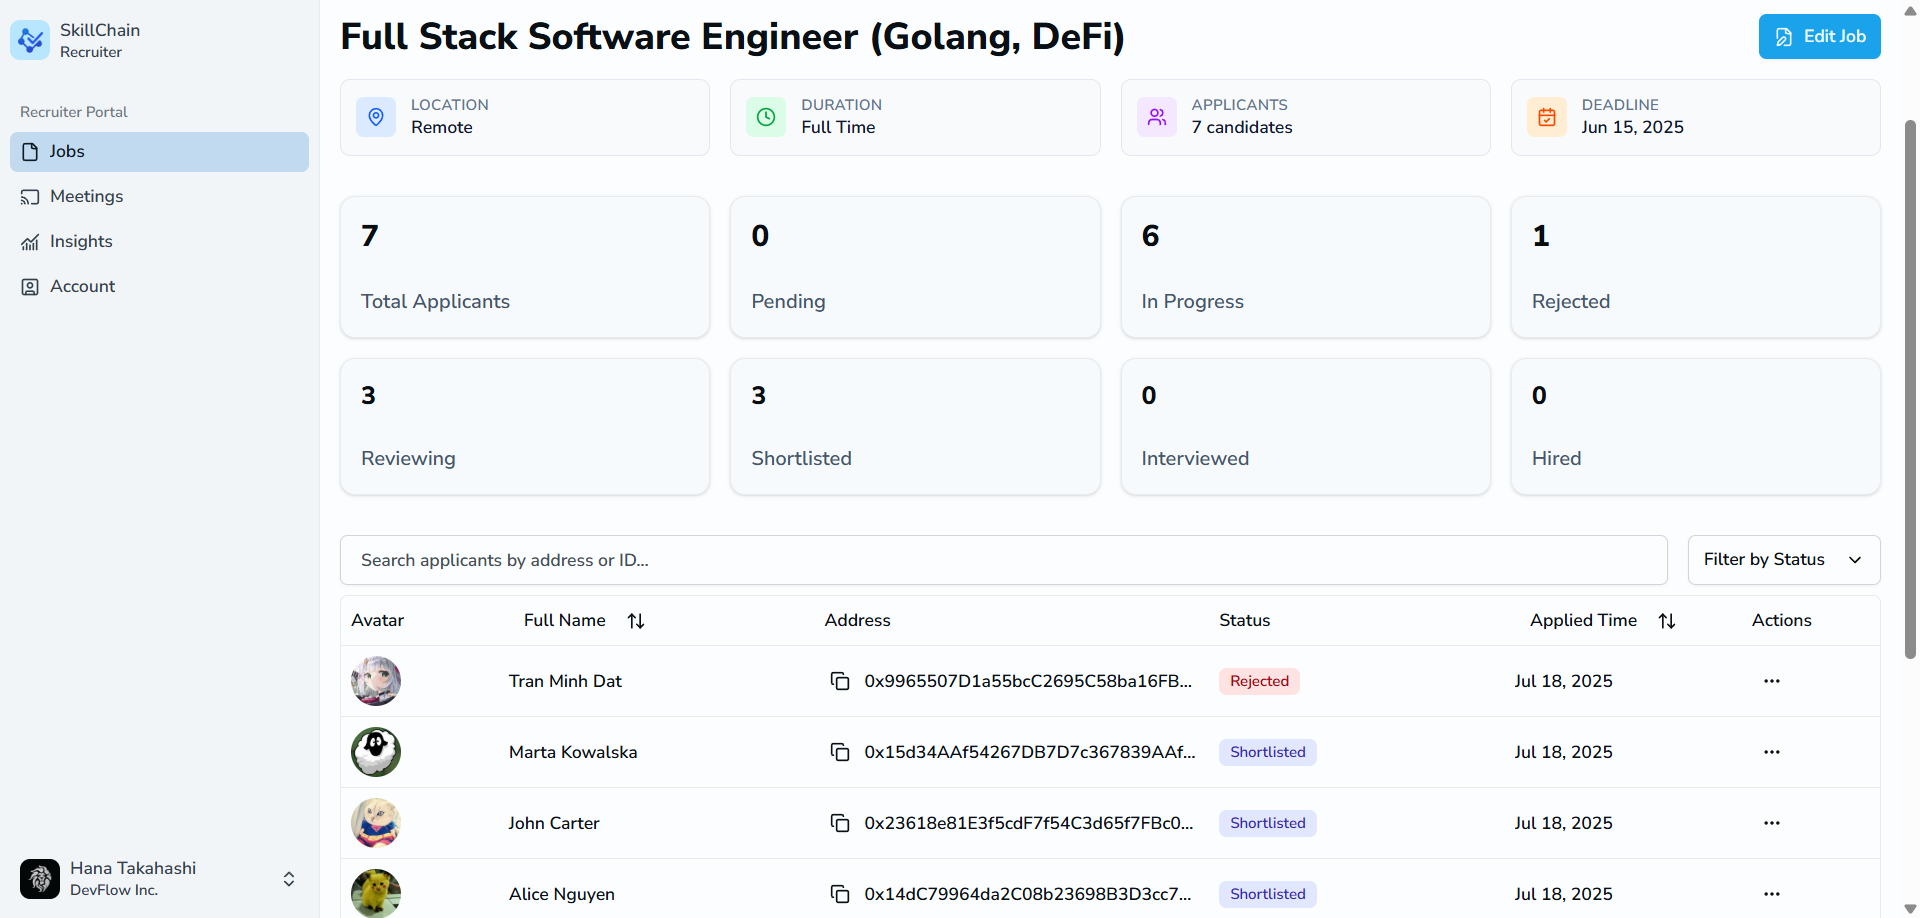
\includegraphics[width=0.99\textwidth, frame]{ui/job-applicants-list-page.png}
  \caption{Danh sách ứng viên ứng tuyển cho một bài đăng}
  \label{fig:job-applicants-list-page}
\end{figure}

Để xem chi tiết hồ sơ một ứng viên, nhà tuyển dụng nhấn ``View application'' tại mục ``Actions'' tương ứng trong danh sách.

\begin{figure}[H]
  \centering
  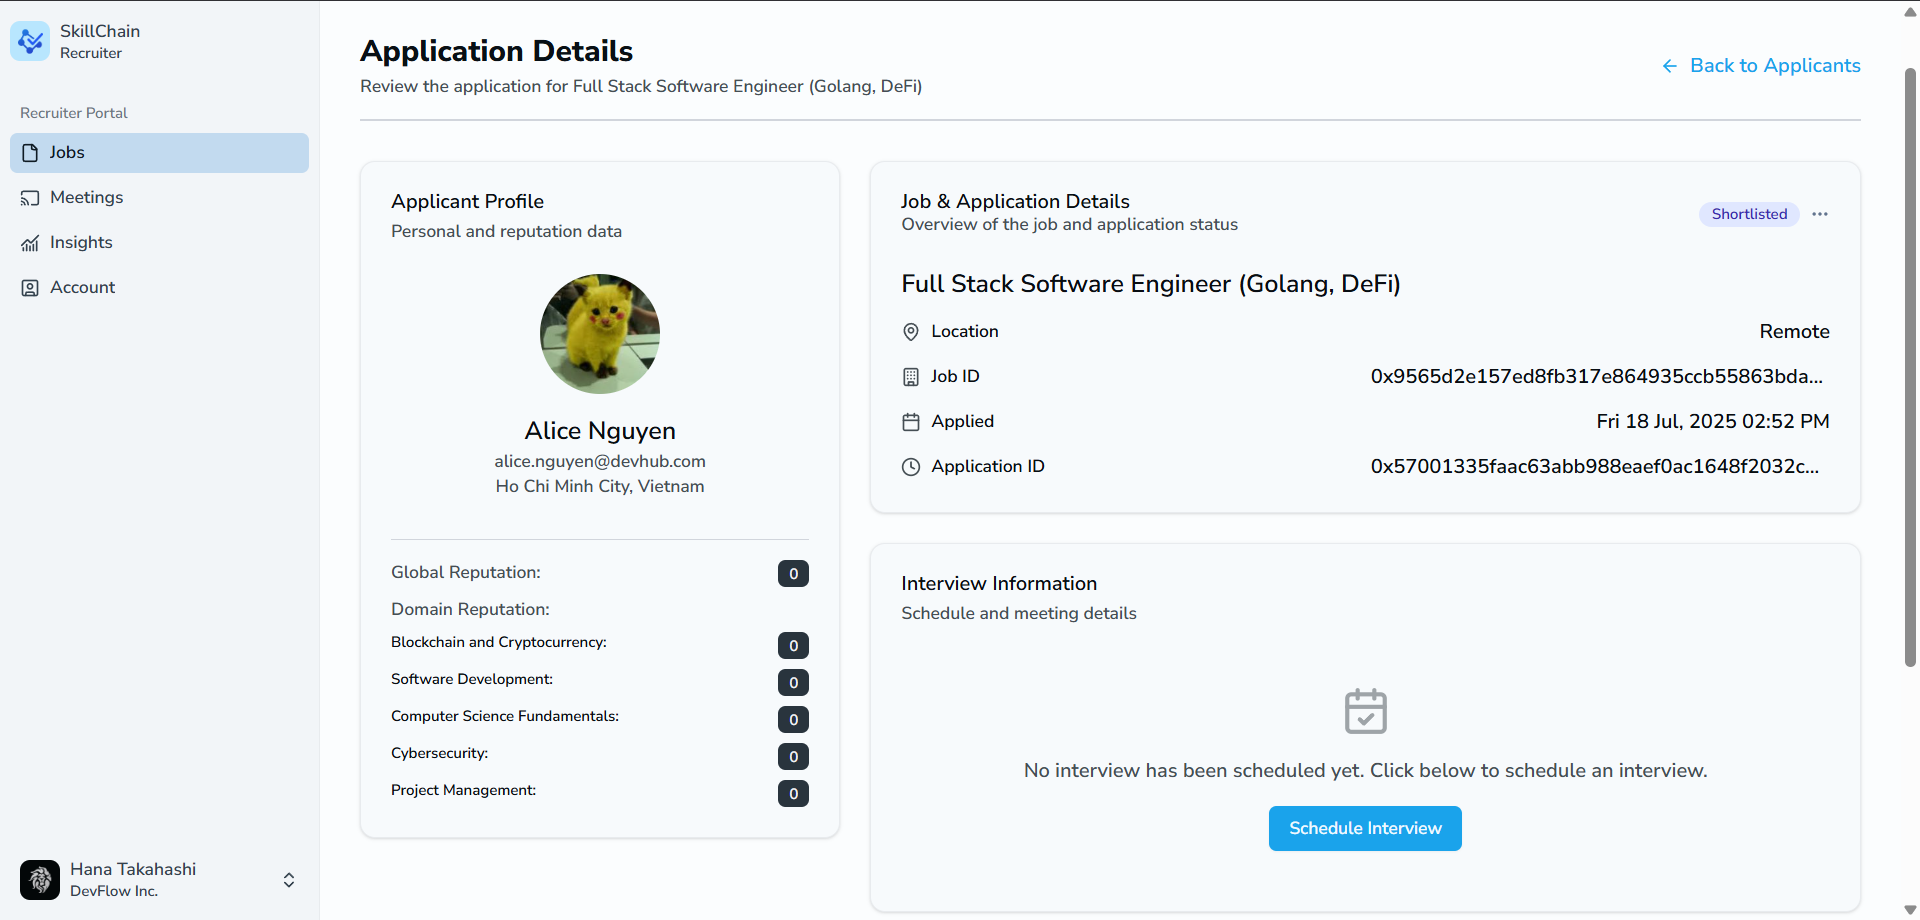
\includegraphics[width=0.99\textwidth, frame]{ui/job-applicant-detail-page.png}
  \caption{Trang chi tiết hồ sơ ứng viên}
  \label{fig:job-applicant-detail-page}
\end{figure}

\subsubsection{Chuyển đổi trạng thái ứng viên}

Tại trang chi tiết hồ sơ ứng viên, để thay đổi trạng thái (ví dụ: từ ``đã đánh giá'' sang ``được rút gọn''), nhà tuyển dụng nhấn biểu tượng ba chấm kế bên thông tin trạng thái trong phần ``Job \& Application Details'' và chọn trạng thái mong muốn.
Hành vi này cần được xác nhận giao dịch thông qua ví tiền điện tử.

\subsection{Quản lý lịch họp trực tuyến}

\subsubsection{Xem danh sách cuộc họp}

Để xem danh sách các cuộc họp đã được lên lịch, nhà tuyển dụng truy cập tab \textbf{Meetings}.  
Tại đây, hệ thống hiển thị danh sách các cuộc họp trực tuyến cùng với các thông tin như trạng thái, vị trí công việc, ứng viên liên quan và thời gian diễn ra.

\begin{figure}[H]
  \centering
  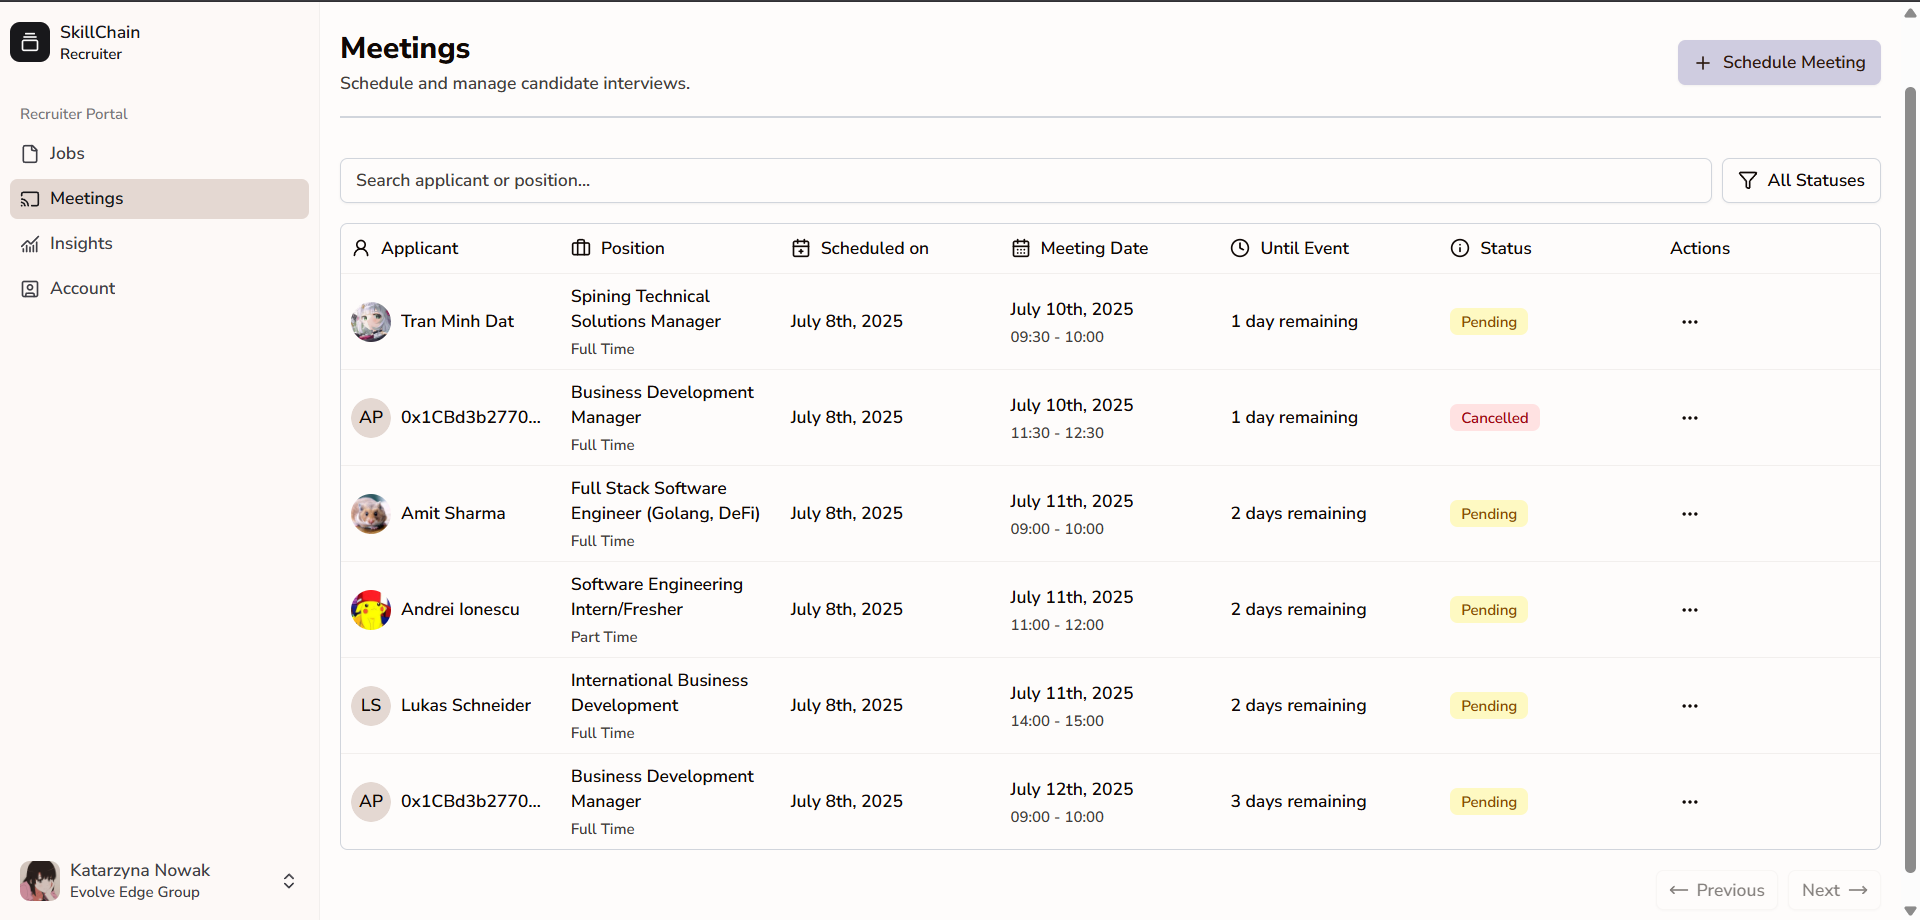
\includegraphics[width=0.99\textwidth, frame]{ui/meeting-list-page.png}
  \caption{Trang danh sách các cuộc họp trực tuyến}
  \label{fig:meeting-list-page}
\end{figure}

Để xem chi tiết một cuộc họp, nhà tuyển dụng nhấn ``View meeting'' tại mục ``Actions'' tương ứng.

\begin{figure}[H]
  \centering
  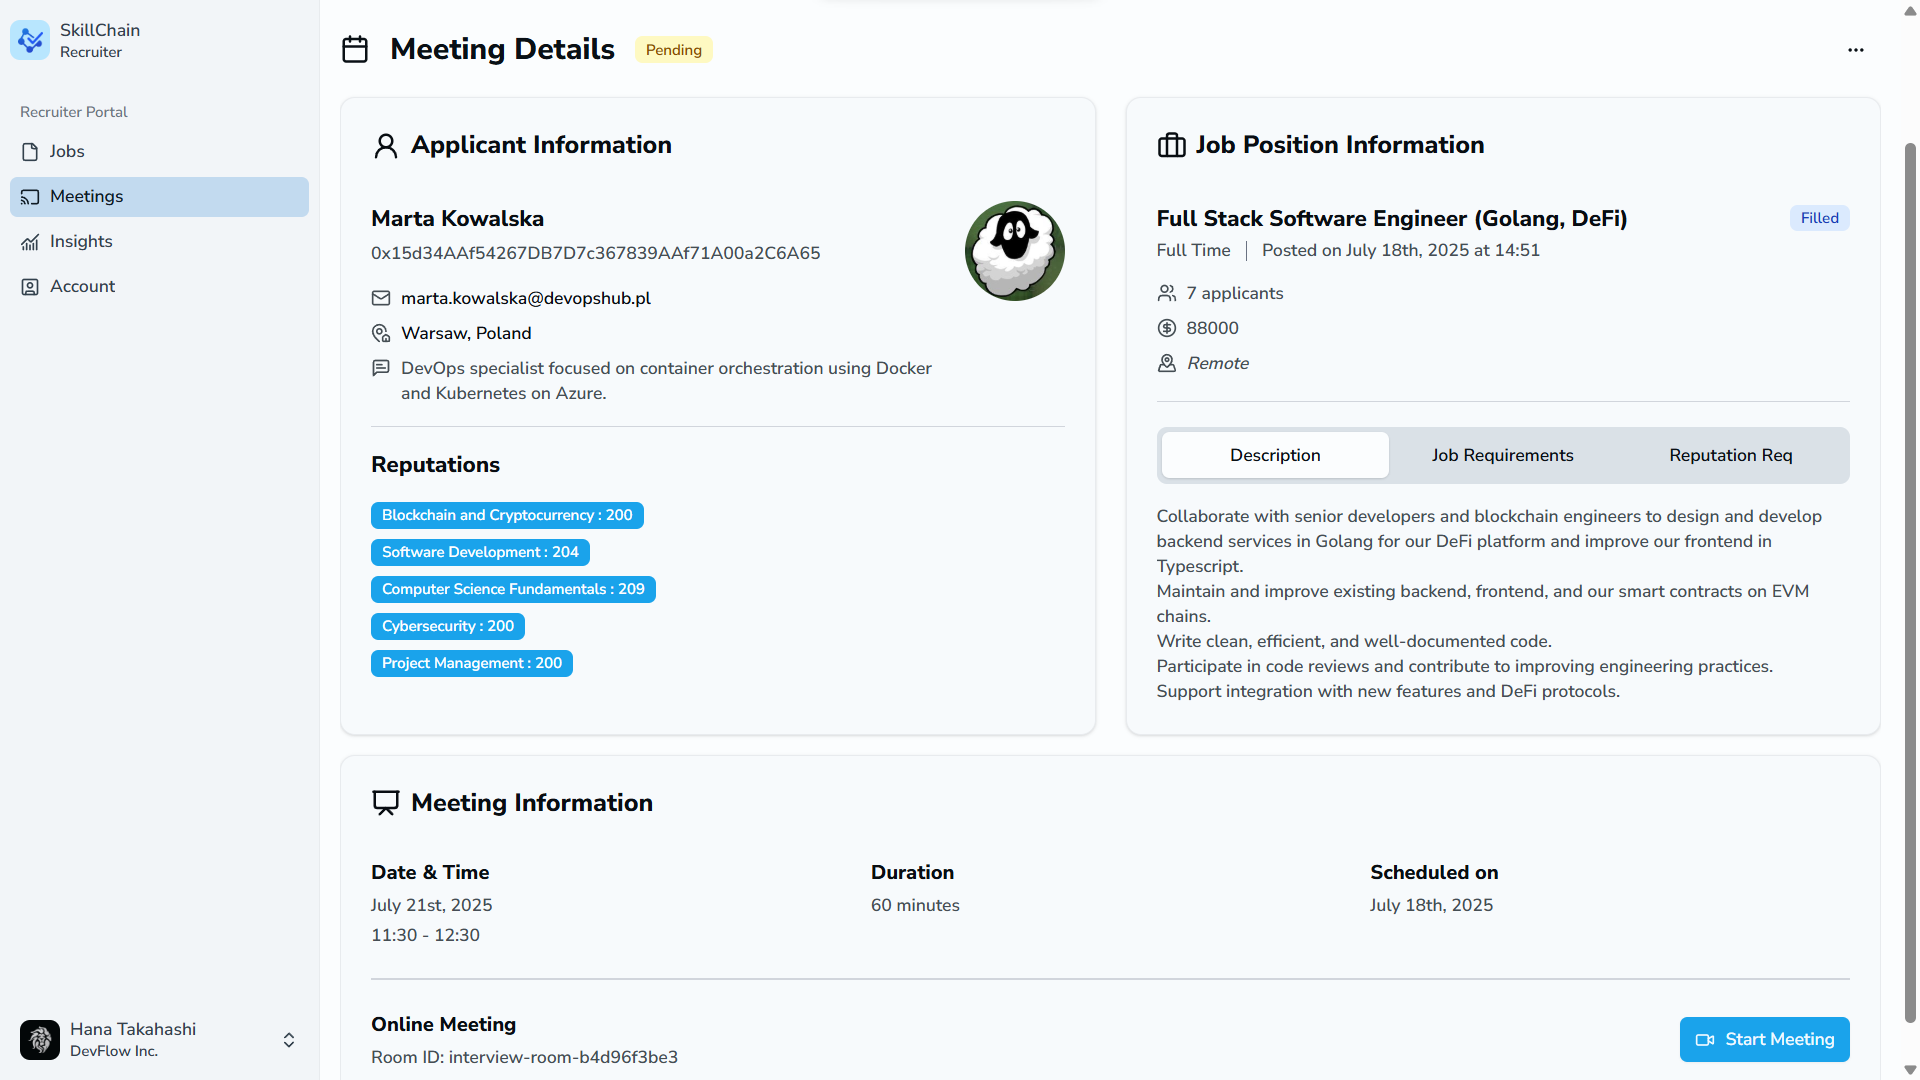
\includegraphics[width=0.99\textwidth, frame]{ui/meeting-detail-page.png}
  \caption{Trang chi tiết một cuộc họp trực tuyến}
  \label{fig:meeting-detail-page}
\end{figure}

Tại trang chi tiết cuộc họp, nhà tuyển dụng có thể đánh dấu trạng thái cuộc họp là \textit{Completed} (Đã hoàn thành) hoặc \textit{Cancelled} (Đã huỷ) bằng cách chọn biểu tượng ba chấm ở góc trên bên phải và thực hiện lựa chọn tương ứng.  
Hành động này yêu cầu xác nhận giao dịch qua ví điện tử.

\subsubsection{Lên lịch một cuộc họp mới}

Để lên lịch một cuộc họp mới, nhà tuyển dụng nhấn nút ``Schedule Meeting'' ở góc trên bên phải trang danh sách cuộc họp.

Tại biểu mẫu lên lịch, nhà tuyển dụng thực hiện các bước:
\begin{enumerate}
  \item Chọn vị trí công việc tương ứng.
  \item Chọn ứng viên thuộc \textbf{danh sách rút gọn} của vị trí đó.
  \item Chọn thời gian diễn ra cuộc họp.
  \item (Tuỳ chọn) Ghi chú gửi đến ứng viên.
\end{enumerate}

Sau khi hoàn tất, nhấn nút ``Schedule'' và xác nhận giao dịch qua ví điện tử để hoàn tất việc lên lịch.

\textbf{Lưu ý:} Nhà tuyển dụng không thể lên lịch một cuộc họp mới cho cùng một ứng viên nếu đã có cuộc họp đang chờ với ứng viên đó.

\begin{figure}[H]
  \centering
  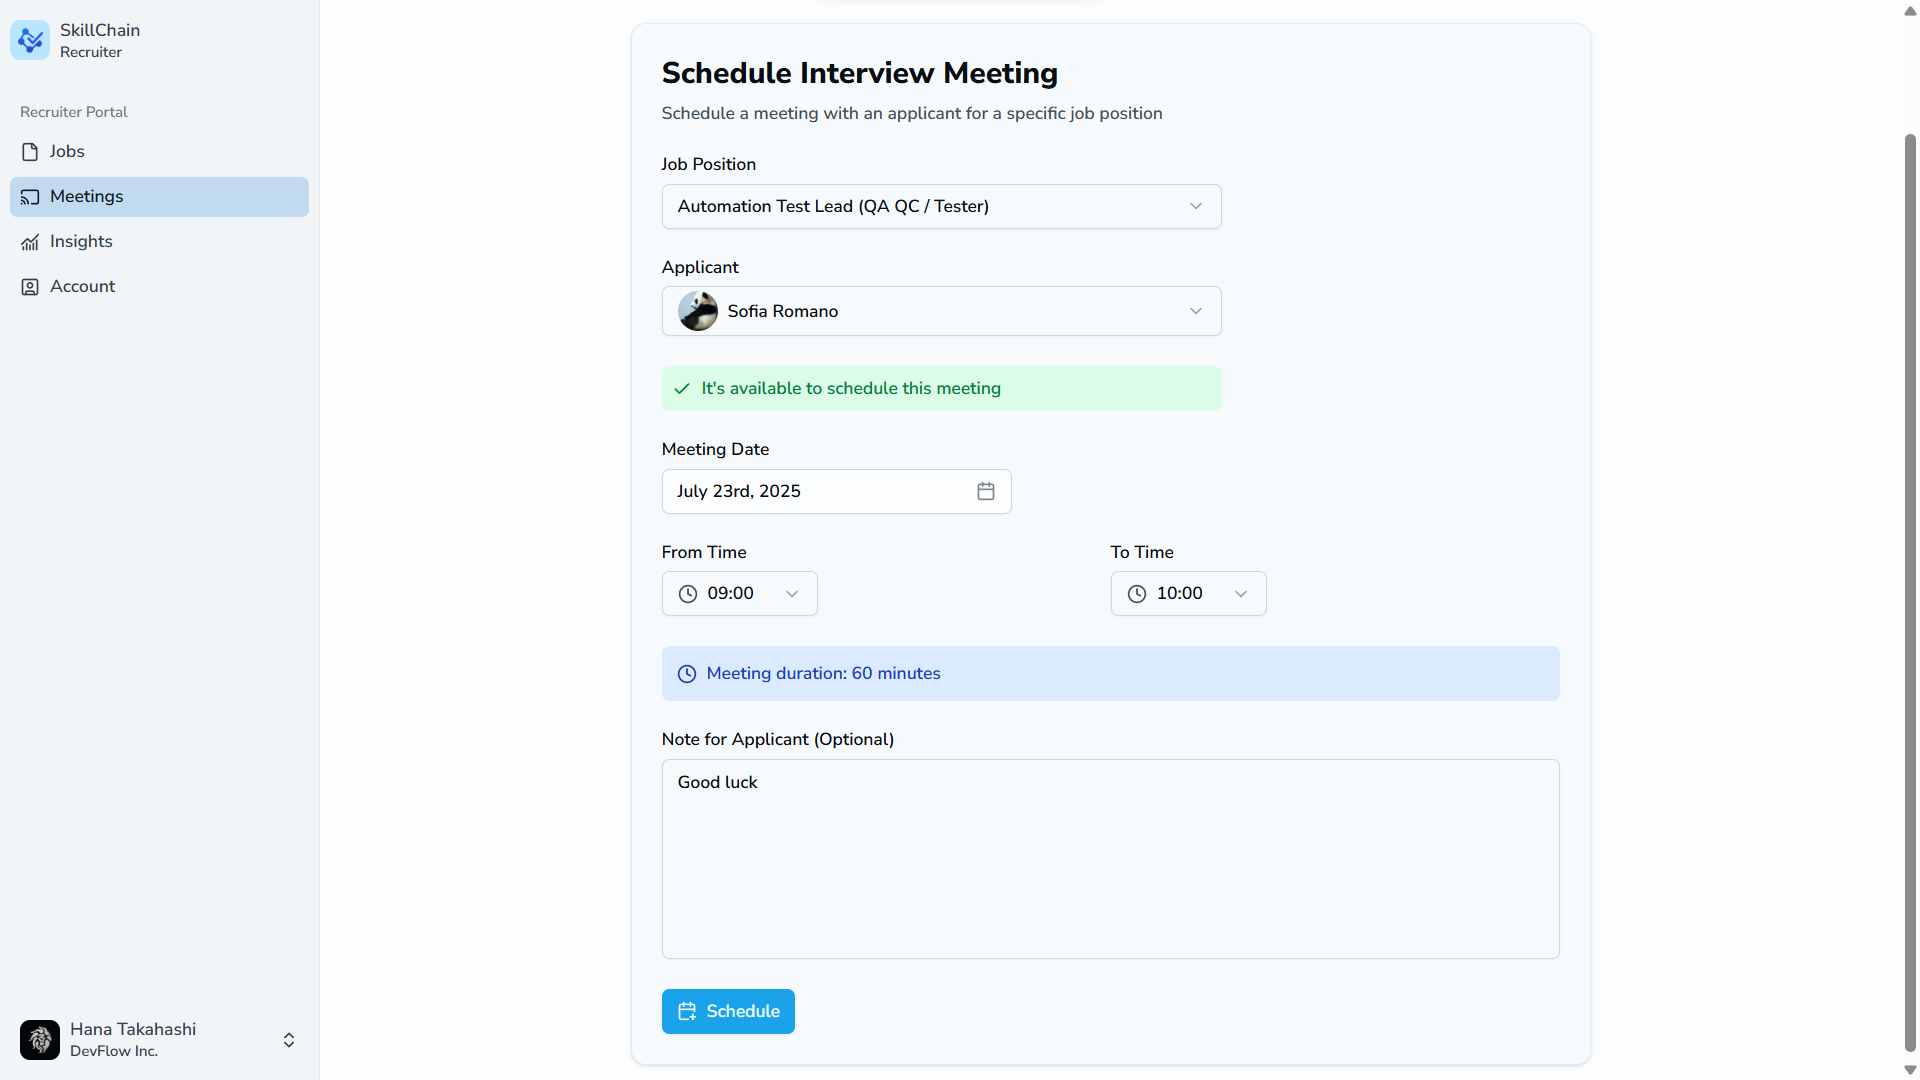
\includegraphics[width=0.99\textwidth, frame]{ui/schedule-meeting-form.png}
  \caption{Biểu mẫu lên lịch cuộc họp}
  \label{fig:schedule-meeting-form}
\end{figure}

\subsubsection{Đổi lịch một cuộc họp}

Đối với các cuộc họp ở trạng thái \textbf{đang chờ}, nhà tuyển dụng có thể thay đổi thời gian họp hoặc ghi chú bằng một trong hai cách:
\begin{itemize}
  \item Từ danh sách cuộc họp, chọn ``Reschedule'' tại mục ``Actions''.
  \item Từ trang chi tiết cuộc họp, nhấn ``Reschedule'' tại biểu tượng ba chấm ở góc trên bên phải.
\end{itemize}

\textbf{Lưu ý:} Không thể thay đổi vị trí công việc hoặc ứng viên đã được chọn.

\begin{figure}[H]
  \centering
  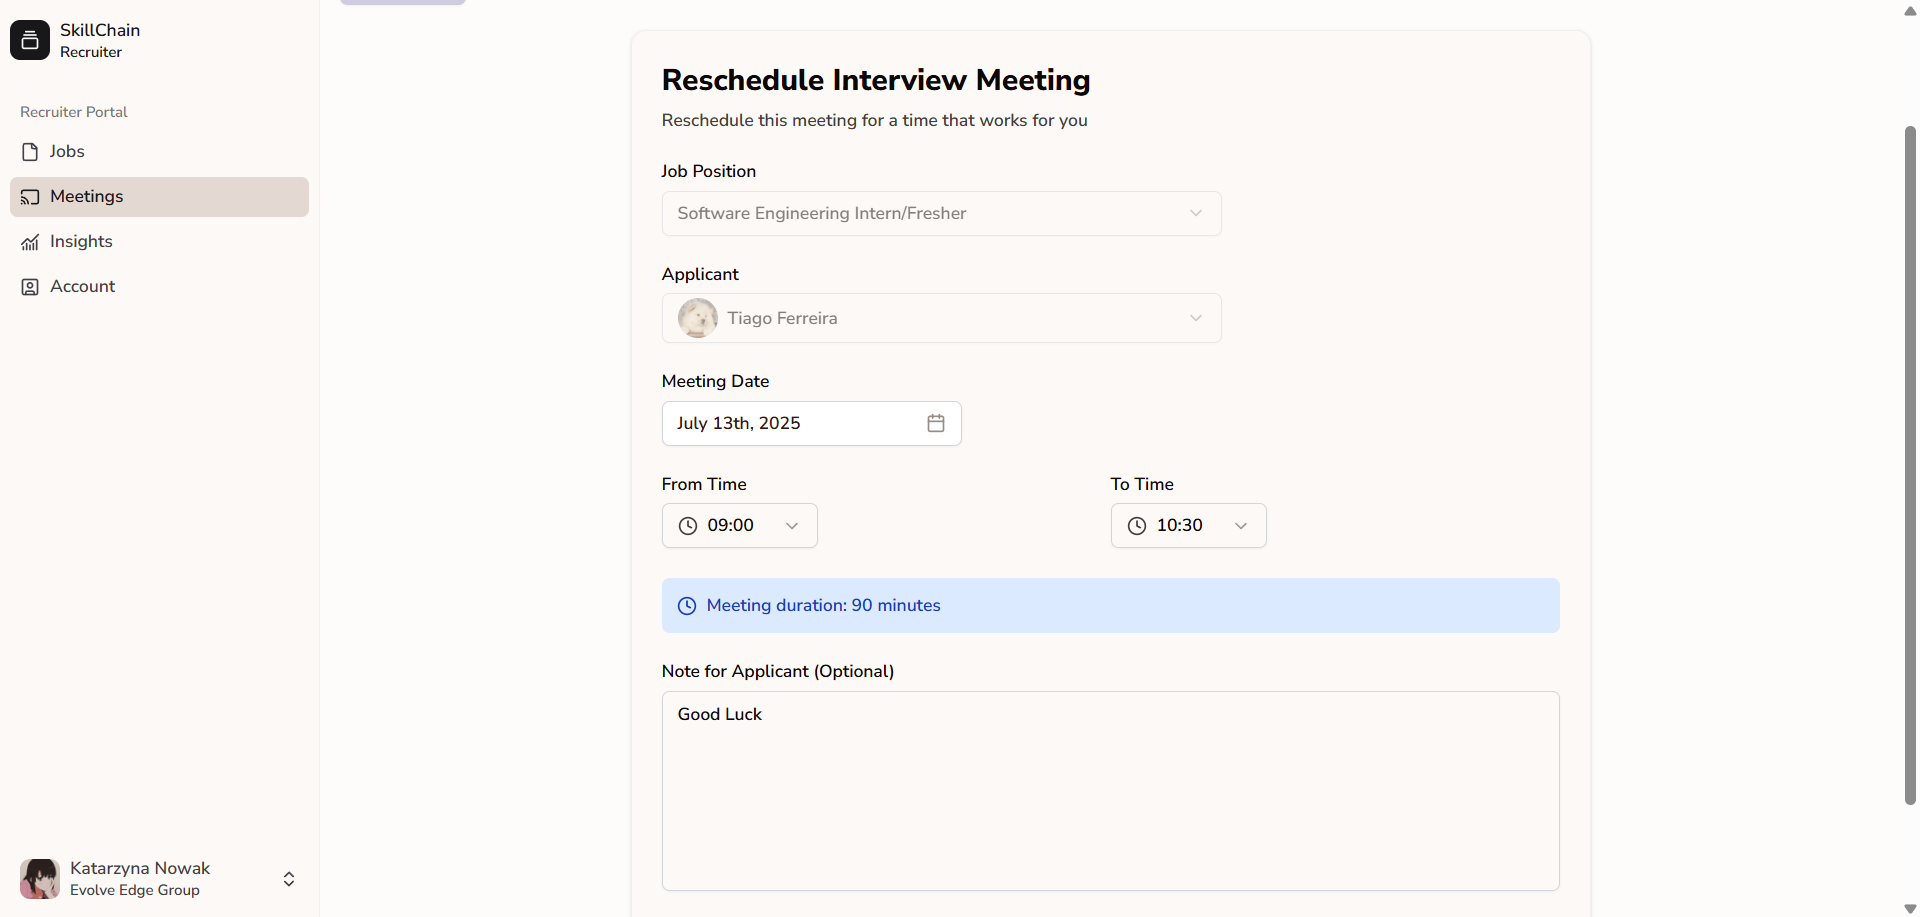
\includegraphics[width=0.99\textwidth, frame]{ui/reschedule-meeting-form.png}
  \caption{Biểu mẫu thay đổi lịch họp}
  \label{fig:reschedule-meeting-form}
\end{figure}

\subsubsection{Triển khai cuộc họp}

Khi đến thời điểm họp, tại trang chi tiết cuộc họp, nhà tuyển dụng nhấn nút ``Start Meeting'' để tạo và khởi chạy phòng họp trực tuyến.  
Hệ thống sẽ tạo liên kết tham gia và gửi đến ứng viên tương ứng.

\begin{figure}[H]
  \centering
  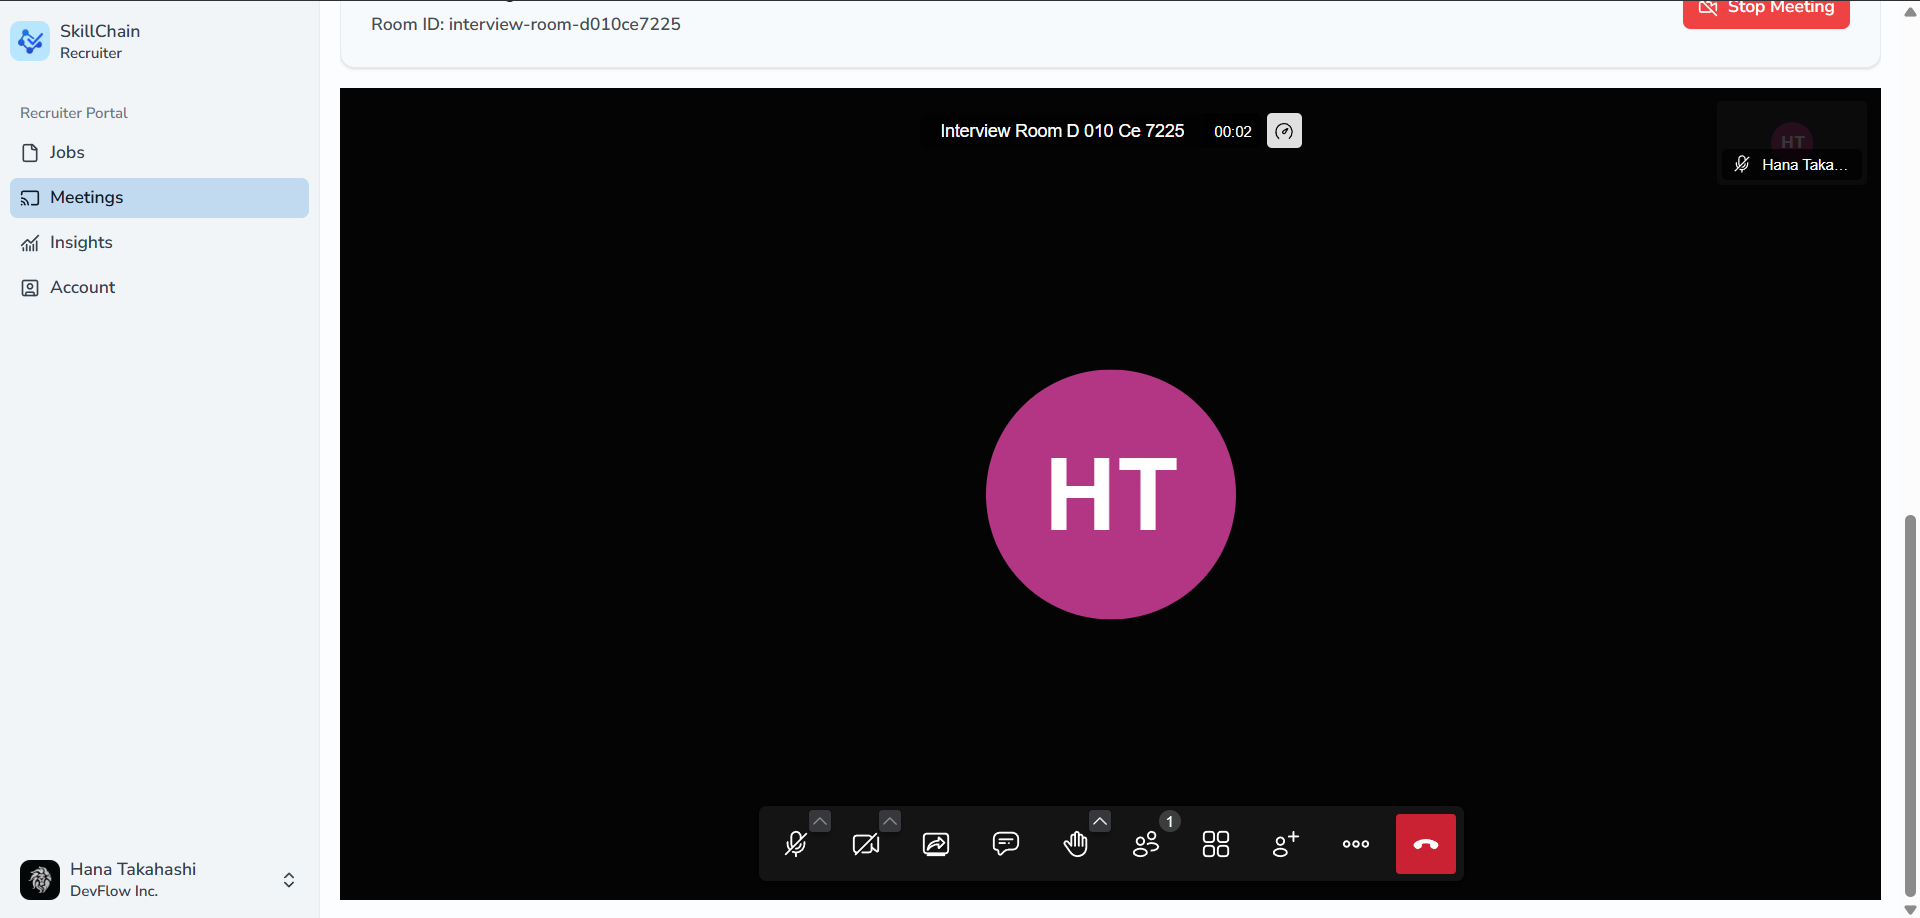
\includegraphics[width=0.99\textwidth, frame]{ui/meeting-hosting.png}
  \caption{Khởi chạy phòng họp trực tuyến}
  \label{fig:meeting-hosting}
\end{figure}

\subsection{Số liệu thống kê}

Để xem các số liệu thống kê liên quan đến quá trình tuyển dụng, nhà tuyển dụng truy cập tab \textbf{Insights}.  
Tại đây, hệ thống hiển thị các chỉ số tổng quan giúp đánh giá hiệu quả hoạt động tuyển dụng.
Bốn chỉ số mặc định được hiển thị gồm:
\begin{itemize}
  \item \textbf{Active Jobs}: Số lượng bài đăng tuyển dụng đang hoạt động.
  \item \textbf{Total Applicants}: Tổng số lượng ứng viên đã ứng tuyển.
  \item \textbf{Conversion Rate}: Tỷ lệ chuyển đổi từ ứng tuyển sang đã tuyển.
  \item \textbf{Pending Meetings}: Số lượng cuộc họp đang chờ diễn ra.
\end{itemize}

\begin{figure}[H]
  \centering
  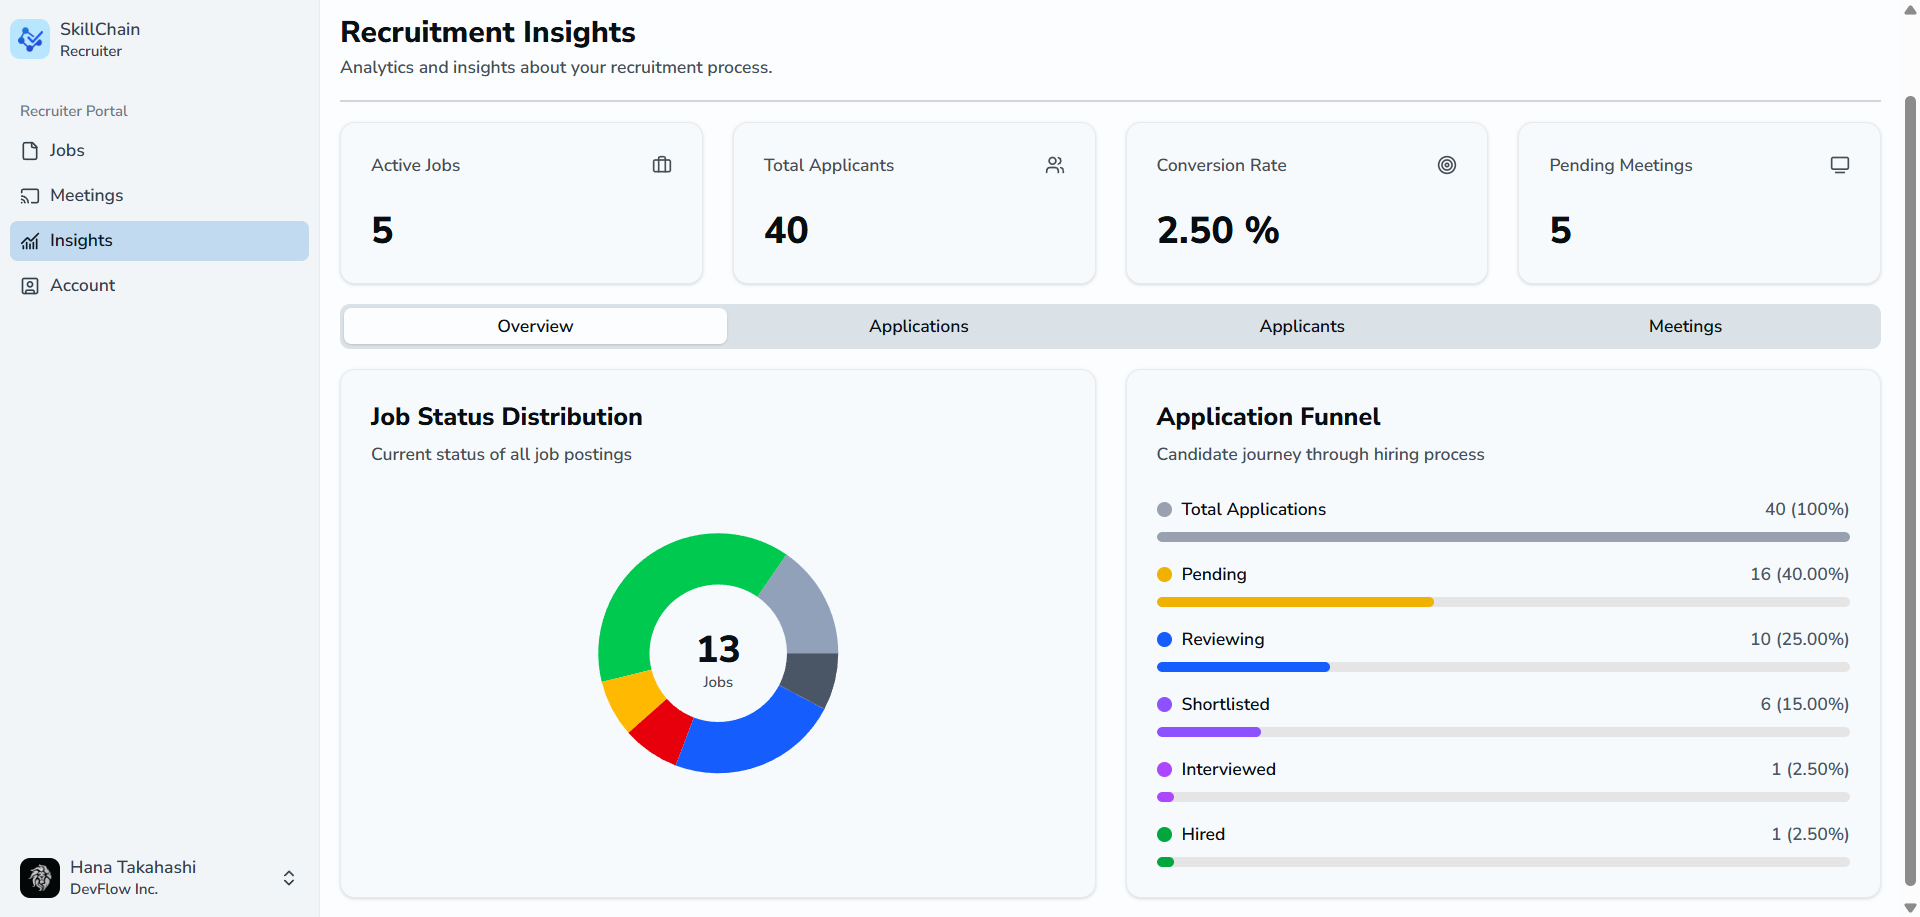
\includegraphics[width=0.99\textwidth, frame]{ui/recruiment-insight-page.png}
  \caption{Trang thống kê quá trình tuyển dụng}
  \label{fig:recruiment-insight-page}
\end{figure}

\subsubsection{Tab tổng quan (Overview)}

Tab \textbf{Overview} hiển thị hai biểu đồ trực quan:
\begin{itemize}
  \item \textbf{Job Status Distribution}: Biểu đồ tròn thể hiện số lượng các trạng thái bài đăng tuyển dụng (đang mở, đã đóng, nháp, v.v.).
  \item \textbf{Application Funnel}: Biểu đồ hình phễu mô tả tỷ lệ và số lượng ứng viên ở một số giai đoạn trong quy trình tuyển dụng.
\end{itemize}

\subsubsection{Tab ứng tuyển (Applications)}

Tab \textbf{Applications} hiển thị danh sách \textbf{Top 5 công việc có hiệu suất tốt nhất}, dựa trên:
\begin{itemize}
  \item Số lượng ứng viên ứng tuyển.
  \item Tỷ lệ chuyển đổi từ ứng viên sang đã tuyển dụng.
\end{itemize}

\begin{figure}[H]
  \centering
  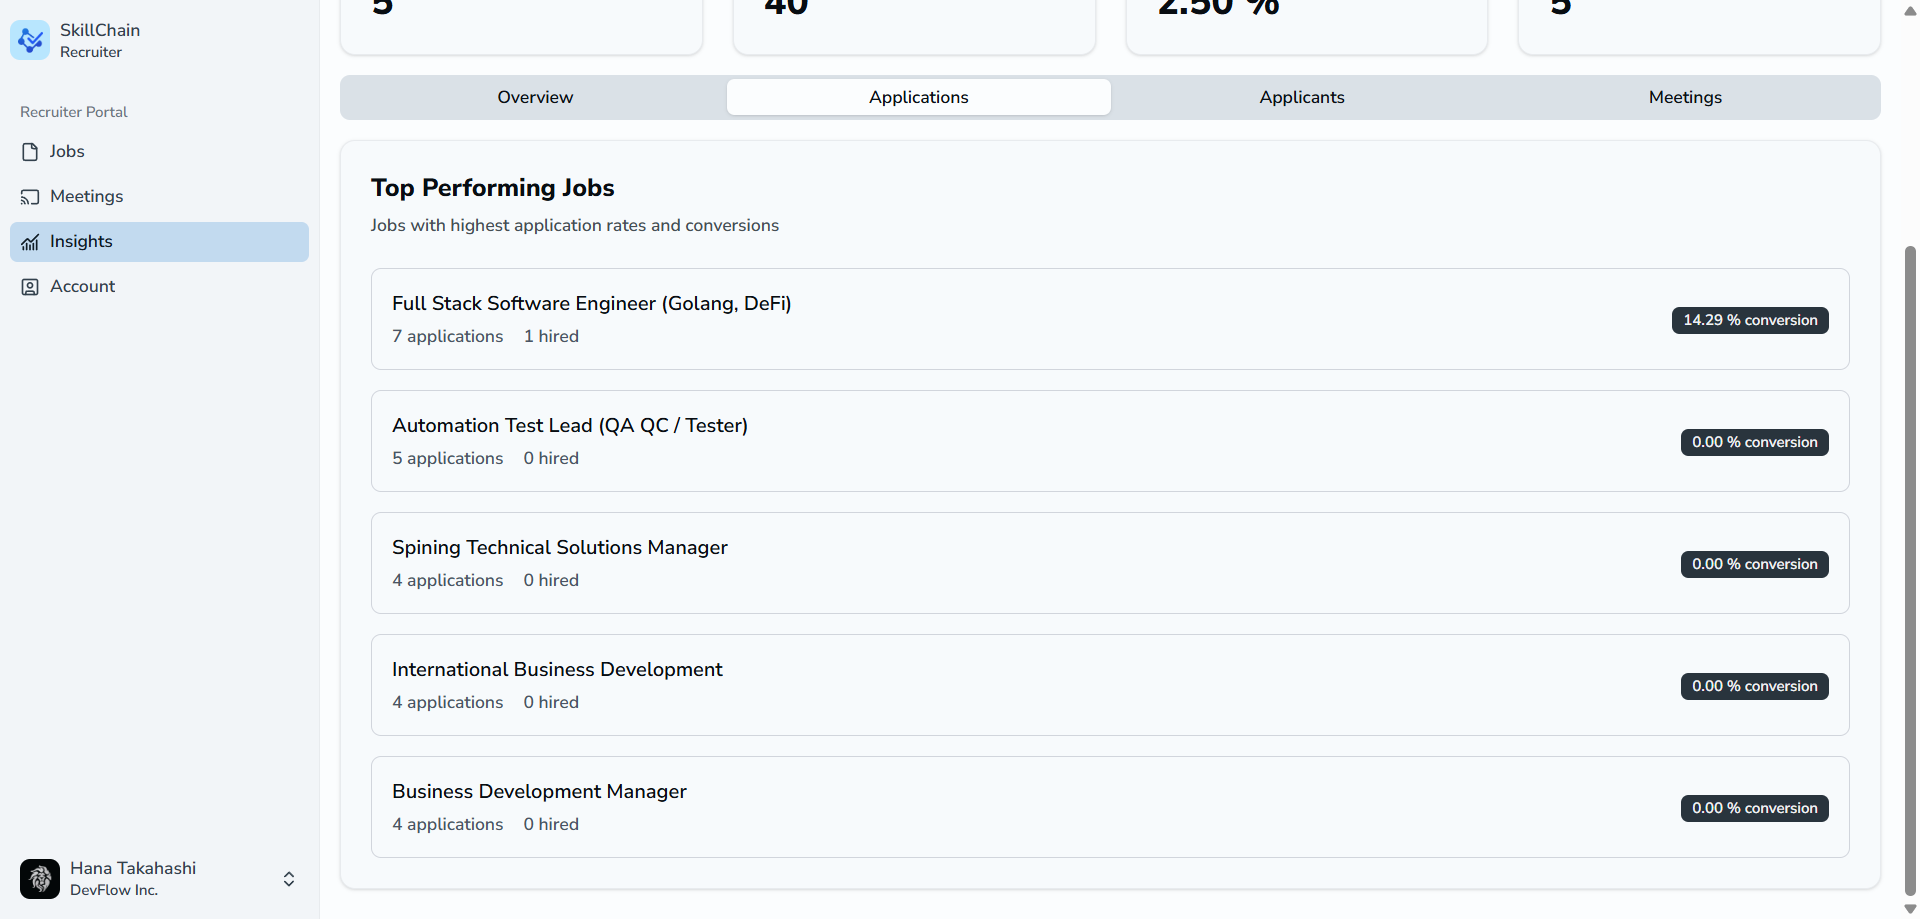
\includegraphics[width=0.99\textwidth, frame]{ui/top-performing-jobs.png}
  \caption{Năm công việc có hiệu suất tuyển dụng cao nhất}
  \label{fig:top-performing-jobs}
\end{figure}

\subsubsection{Tab ứng viên (Applicants)}

Tab \textbf{Applicants} hiển thị \textbf{Top 5 ứng viên tương tác nhiều nhất}, được đánh giá dựa trên số lượng bài đăng từ nhà tuyển dụng mà họ đã ứng tuyển.

\begin{figure}[H]
  \centering
  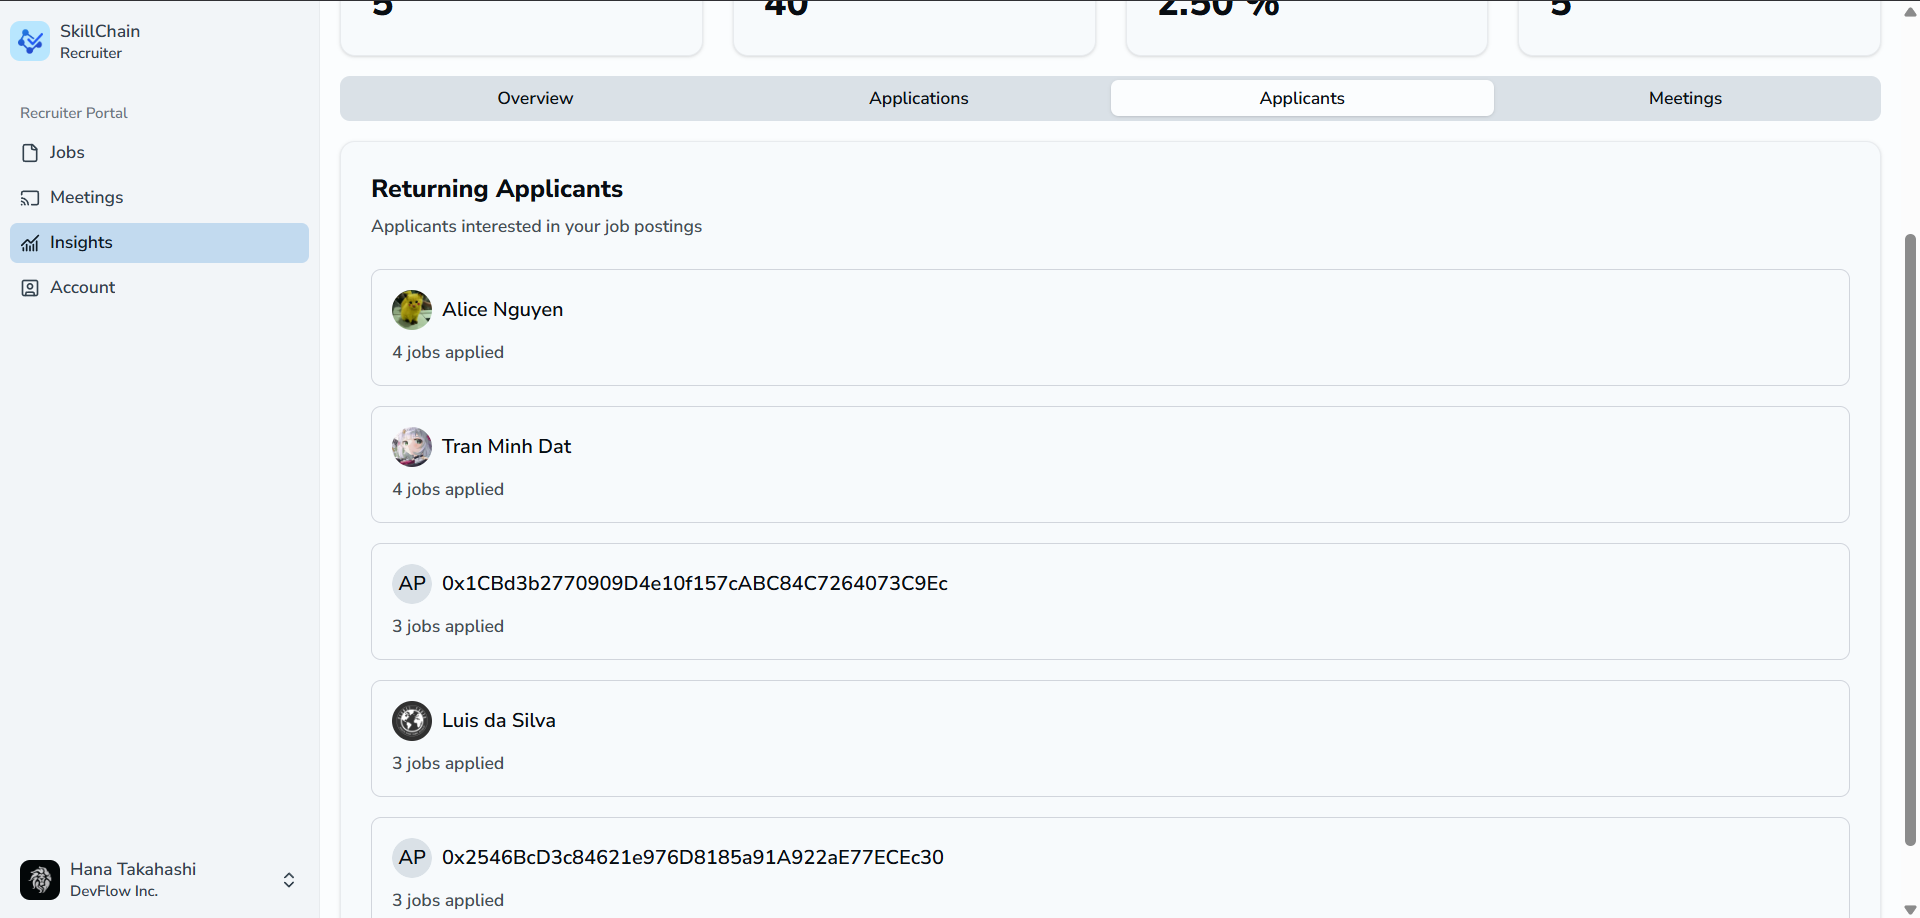
\includegraphics[width=0.99\textwidth, frame]{ui/top-returning-applicants.png}
  \caption{Năm ứng viên tương tác nhiều nhất với nhà tuyển dụng}
  \label{fig:top-returning-applicants}
\end{figure}

\subsubsection{Tab cuộc họp (Meetings)}

Tab \textbf{Meetings} cung cấp:
\begin{itemize}
  \item \textbf{Meeting Status Distribution}: Biểu đồ phân bố trạng thái các cuộc họp (đã hoàn thành, đang chờ, đã huỷ).
  \item \textbf{Upcoming Meetings}: Danh sách những cuộc họp sắp diễn ra, giúp nhà tuyển dụng chủ động chuẩn bị.
\end{itemize}

\begin{figure}[H]
  \centering
  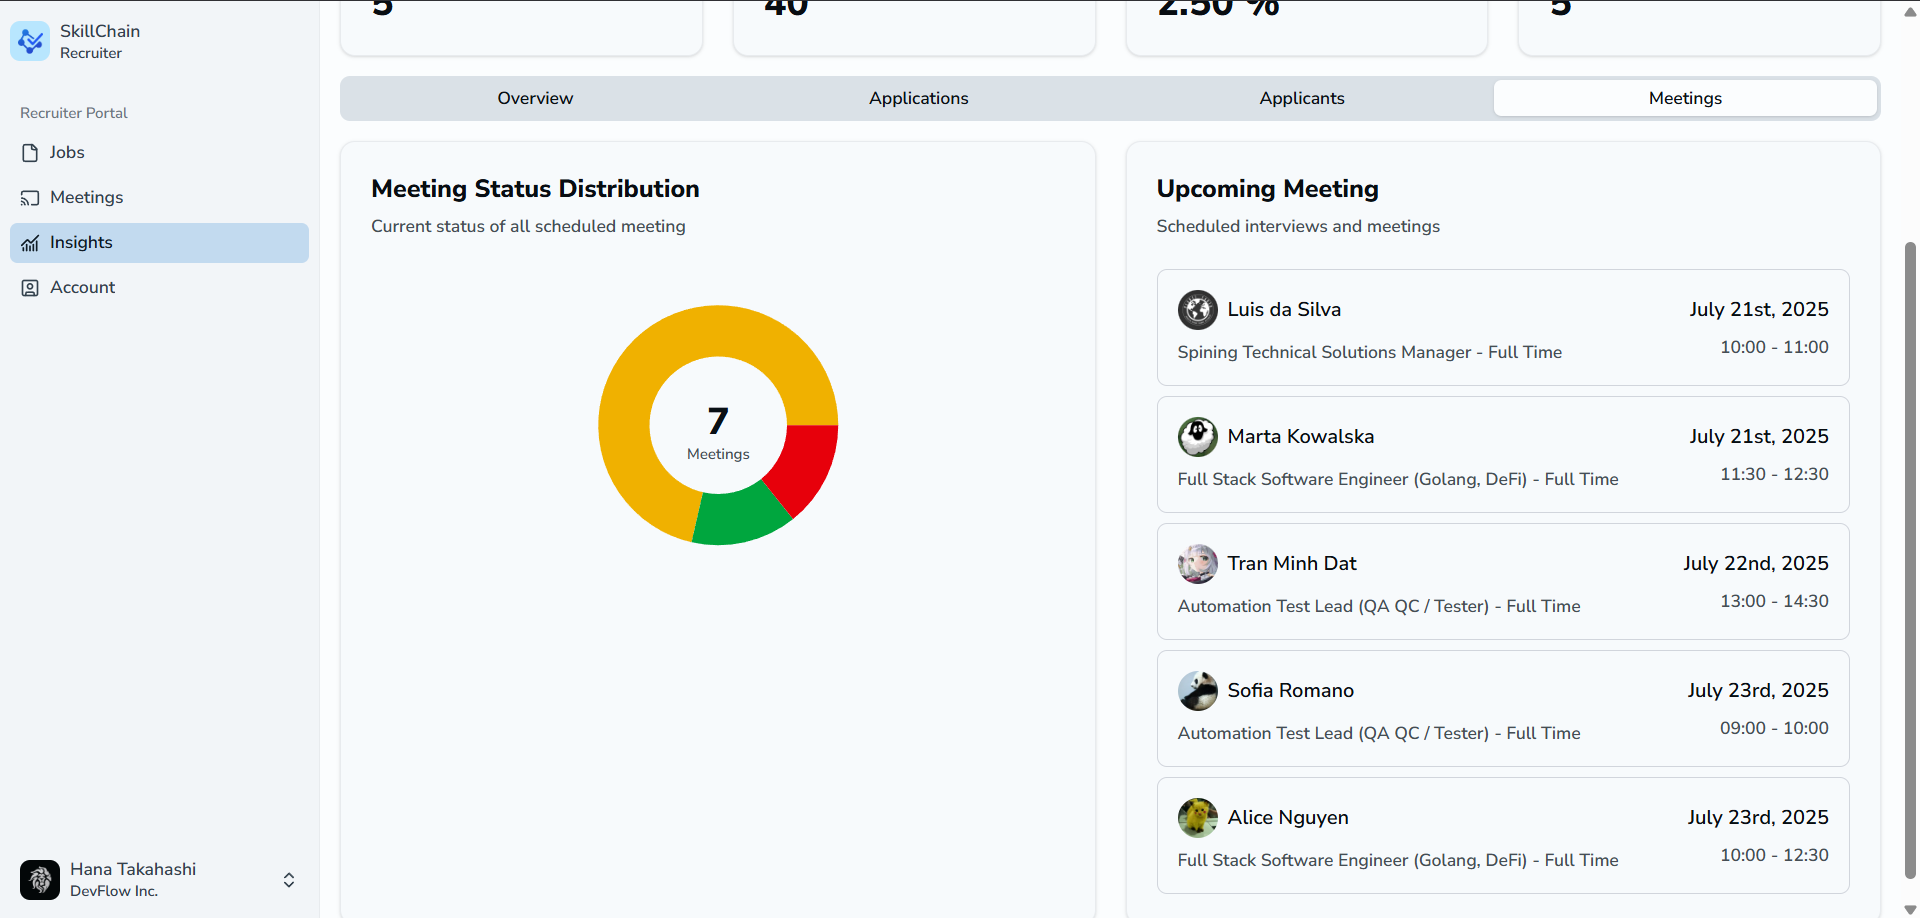
\includegraphics[width=0.99\textwidth, frame]{ui/insight-meetings-tab.png}
  \caption{Thống kê về các cuộc họp phỏng vấn}
  \label{fig:insight-meetings-tab}
\end{figure}

\subsection{Người dùng tham gia ứng tuyển}

\subsubsection{Xem danh sách công việc đang mở}

Để xem danh sách các công việc đang tuyển dụng, người dùng truy cập \textbf{Career} $\rightarrow$ \textbf{Available Jobs} trong không gian xây dựng uy tín.

\begin{figure}[H]
  \centering
  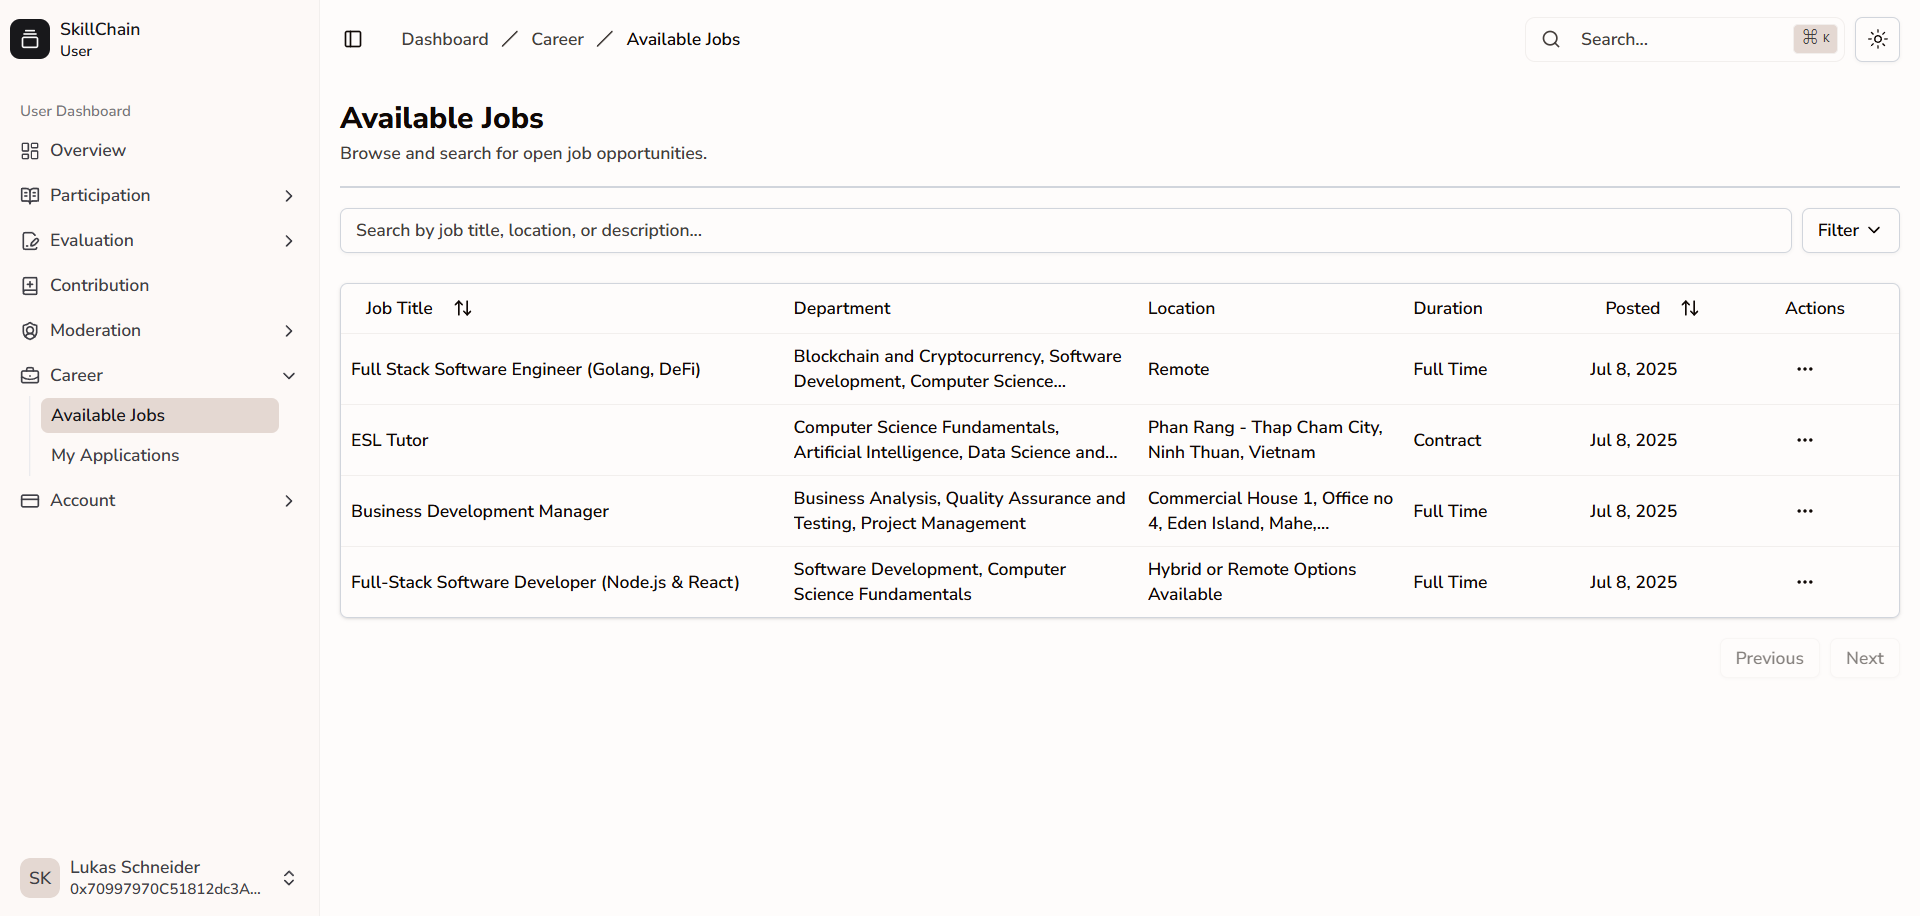
\includegraphics[width=0.99\textwidth, frame]{ui/available-jobs-page.png}
  \caption{Trang các công việc đang mở}
  \label{fig:available-jobs-page}
\end{figure}

Tại đây, người dùng có thể xem thông tin cơ bản của từng công việc như vị trí tuyển dụng, yêu cầu uy tín hay thời gian làm việc. 
Để xem chi tiết, nhấn nút ``View job'' tại mục ``Actions'' tương ứng.

\begin{figure}[H]
  \centering
  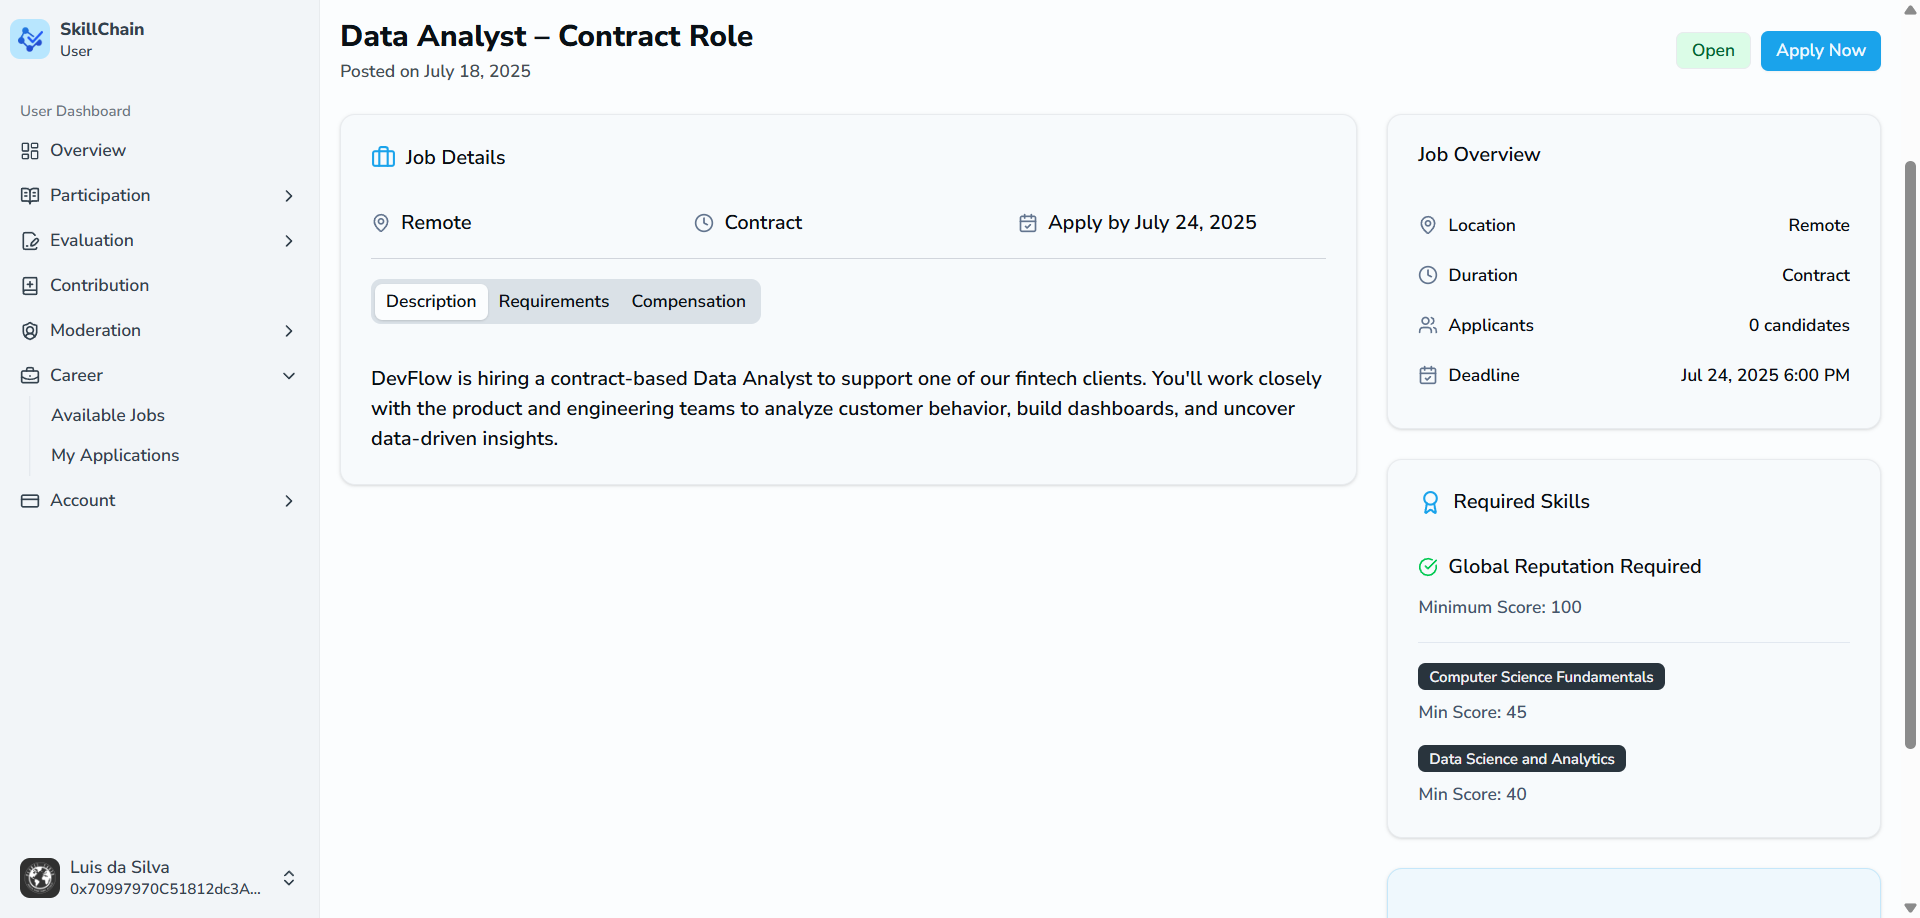
\includegraphics[width=0.99\textwidth, frame]{ui/available-job-detail-page.png}
  \caption{Trang chi tiết một công việc}
  \label{fig:available-job-detail-page}
\end{figure}

\subsubsection{Tham gia ứng tuyển}

Khi truy cập trang chi tiết công việc, hệ thống sẽ tự động kiểm tra mức độ uy tín của người dùng. Nếu không đáp ứng yêu cầu, hệ thống sẽ hiển thị thông báo và vô hiệu hóa nút ứng tuyển. 
Nếu đủ điều kiện, người dùng có thể nhấn nút ``Apply'' ở góc trên bên phải để nộp đơn ứng tuyển. Hành vi này yêu cầu xác nhận giao dịch thông qua ví tiền điện tử.

\subsubsection{Xem các công việc đã ứng tuyển}

Để theo dõi các công việc đã ứng tuyển, người dùng truy cập \textbf{Career} $\rightarrow$ \textbf{My Applications}. Tại đây, hệ thống hiển thị danh sách các công việc mà người dùng đã nộp đơn cùng với trạng thái tương ứng.

\begin{figure}[H]
  \centering
  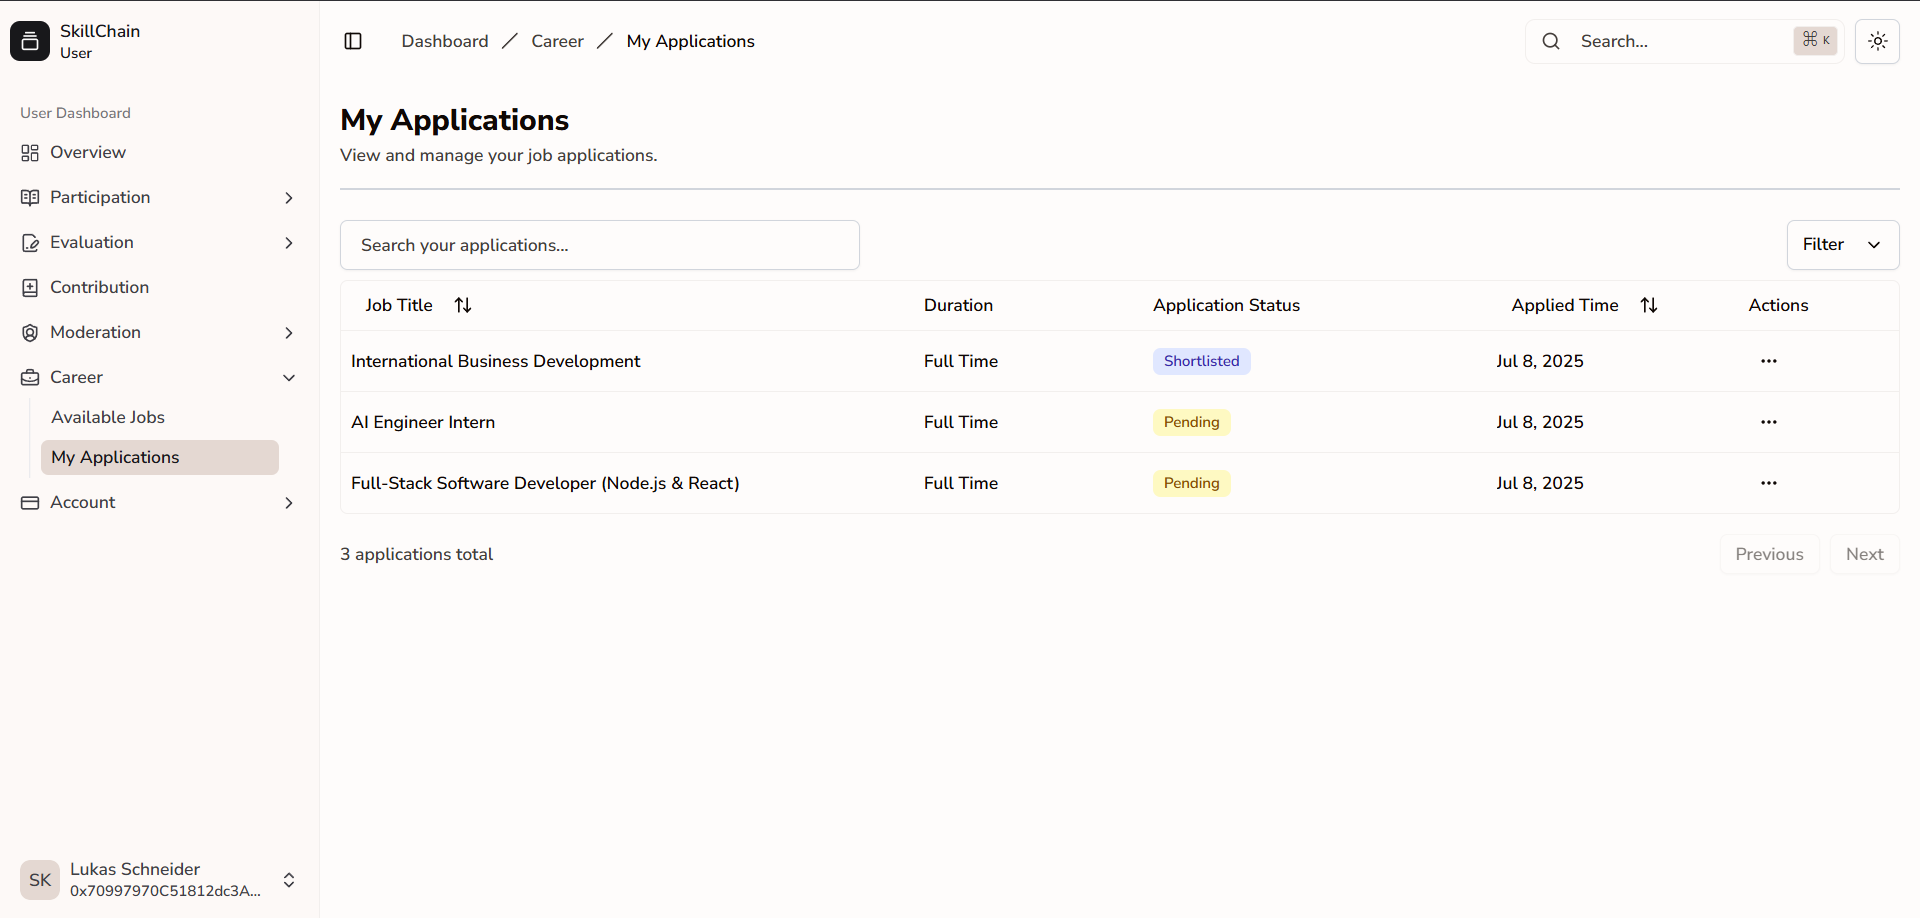
\includegraphics[width=0.99\textwidth, frame]{ui/my-applications-page.png}
  \caption{Trang công việc đã ứng tuyển}
  \label{fig:my-applications-page}
\end{figure}

Để xem thông tin chi tiết của một đơn ứng tuyển, nhấn ``View application'' tại nút ``Actions'' của công việc tương ứng. 
Trong trường hợp người dùng được đưa vào danh sách rút gọn, hệ thống sẽ hiển thị thêm thông tin lịch họp và liên kết tham gia phòng họp trực tuyến (nếu nhà tuyển dụng đã lên lịch).

\begin{figure}[H]
  \centering
  \includegraphics[width=0.99\textwidth, frame]{ui/my-application-detail-page.png}
  \caption{Trang chi tiết của một đơn ứng tuyển}
  \label{fig:my-application-detail-page}
\end{figure}

\subsubsection{Rút đơn ứng tuyển}

Nếu người dùng muốn hủy ứng tuyển, có thể nhấn nút ``Withdraw Application'' ở góc trên bên phải tại trang chi tiết ứng tuyển. Hành vi này yêu cầu xác nhận giao dịch thông qua ví tiền điện tử.
Người dùng sau đó sẽ không thể ứng tuyển lại cho vị trí này nữa.